\documentclass{article}
%\usepackage[top=30pt,left=30pt,right=30pt]{geometry}
\usepackage[german,english]{babel}
\usepackage[utf8]{inputenc}
\usepackage{algpseudocode}
\usepackage{algorithm}
\usepackage{graphicx}
\usepackage{caption}
\usepackage{subcaption}
\usepackage{amsmath}
\usepackage{amssymb}
\usepackage{enumitem}
\usepackage{amsthm}
\usepackage{pxfonts}
\usepackage{wasysym}
\usepackage{framed}
\usepackage{xcolor}
%\usepackage{eufrak}
\usepackage{makeidx}
\usepackage{csquotes}
\usepackage[pdfborder={0 0 0}]{hyperref}
\usepackage{stmaryrd}
\usepackage{titlesec}
\titleformat{\paragraph}{\normalfont\itshape}{}{}{}

\newtheorem{theorem}{Theorem}  \numberwithin{theorem}{section}
\newtheorem{problem}{Problem}  \numberwithin{problem}{section}
\newtheorem{example}{Example}  \numberwithin{example}{section}
\newtheorem*{hypothesis}{Hypothesis}%  \numberwithin{hypothesis}{section}
\newtheorem{definition}{Definition}  \numberwithin{definition}{section}
\newtheorem{lemma}{Lemma}  \numberwithin{lemma}{section}
\newtheorem*{claim}{Claim}%  \numberwithin{claim}{section}
\newtheorem{remark}{Remark}  \numberwithin{remark}{section}
\newtheorem*{corollary}{Corollary}%  \numberwithin{corollary}{section}
\newtheorem{proposition}{Proposition}  \numberwithin{proposition}{section}

\algnewcommand{\algorithmicgoto}{\textbf{go to}}%
\algnewcommand{\Goto}[1]{\algorithmicgoto~\ref{#1}}%
\algrenewcommand{\algorithmiccomment}[1]{\hskip2em$\triangleright$ {\footnotesize #1}}

% definitions
\newcommand{\drawing}[1]{%
 \begin{figure}[t]
  \begin{center}
   \includegraphics{#1}
  \end{center}
 \end{figure}
}
\newcommand{\pic}[2]{%
 \begin{figure}[t]
  \begin{center}
   \includegraphics{#1}
   \caption{#2}
  \end{center}
 \end{figure}
}
\newcommand{\set}[1]{\left\{#1\right\}}
\newcommand{\setdef}[2]{\left\{\left.#1\,\right|\,#2\right\}}
\newcommand{\ip}[2]{\left\langle#1,#2\right\rangle} % inner product
\newcommand{\angel}[1]{\left\langle#1\right\rangle}
\newcommand{\norm}[1]{\left\|#1\right\|}
\newcommand{\card}[1]{\left|#1\right|}
\newcommand{\given}[1]{\textbf{Given.} #1\par}
\newcommand{\find}[1]{\textbf{Find.} #1\par}
\newcommand{\dateref}[1]{\paragraph{\textit{This lecture took place on #1.}}}
\newcommand{\exist}{\;\exists\,}
\newcommand{\fall}{\;\forall\,}
\newcommand{\noproof}[1]{A proof for Theorem~\ref{#1} is not provided.}
\newcommand{\vectwo}[2]{\begin{pmatrix} #1 \\ #2 \end{pmatrix}}
\newcommand{\vecthree}[3]{\begin{pmatrix} #1 \\ #2 \\ #3 \end{pmatrix}}
\makeatletter
\newcommand{\xRightarrow}[2][]{\ext@arrow 0359\Rightarrowfill@{#1}{#2}}
\makeatother
\newcommand{\rh}[1]{\vec{#1}}
\newcommand{\sout}[1]{#1} % TODO define a strike-through for math mode

\newcommand{\mtn}{(\mu\times\nu)} % mu times nu

\DeclareMathOperator{\rank}{rank}
\DeclareMathOperator{\detm}{det}
\DeclareMathOperator{\perm}{perm}
\DeclareMathOperator{\sign}{sign}
\DeclareMathOperator{\degree}{deg}
\DeclareMathOperator{\im}{image}
\DeclareMathOperator{\ke}{kern}
\DeclareMathOperator{\prop}{probability}
\DeclareMathOperator{\Hom}{Hom}
\DeclareMathOperator{\argmax}{argmax}
\DeclareMathOperator{\argmin}{argmin}
\DeclareMathOperator{\vol}{vol}  % volume
\DeclareMathOperator*{\bigtimes}{\vartimes}

\makeatletter
\providecommand*{\dotcup}{%
  \mathbin{%
    \mathpalette\@dotcup{}%
  }%
}
\newcommand*{\@dotcup}[2]{%
  \ooalign{%
    $\m@th#1\cup$\cr
    \hidewidth$\m@th#1\cdot$\hidewidth
  }%
}
\makeatother


% metadata
\title{
  Linear Algebra 2 \\
  \large{Lecture notes, University (of Technology) Graz} \\
  based on the lecture by Franz Lehner
}
\date{\today}
\author{Lukas Prokop}

% settings
\parindent0pt
\setlength{\parskip}{0.4\baselineskip}
%\setcounter{tocdepth}{2}

\makeindex

\begin{document}
\maketitle
\tableofcontents

\dateref{2018/03/05}
\subsection{Lecture}

\begin{itemize}
  \item Mon, 08:15--09:45, lecture
  \item Wed, 08:15--09:45, lecture
  \item Mon, 16:00--18:00, tutorial, AE01
  \item Mon, 13:15--14:00, conversatorium (BE01)
\end{itemize}

\section{Linear algebra 1}

Gottfried Wilhelm von Leibniz (1646--1716). Results from 1693:

\begin{itemize}
  \item Vector spaces (first definition in 1880)
  \item Matrices and linear maps
\end{itemize}

From now, it will be more specific (matrices). In general, we discuss \enquote{when is a matrix invertible}?

\begin{align*}
  ax + by &= e \\
  cx + dy &= f
\end{align*}

We need to invert the matrix

Assuming $a \neq 0$. We multiply the first row with $\cdot \frac1a \cdot (-c)$.
\[
  \begin{array}{cc|cc}
    a & b & 1 & 0 \\
    c & d & 0 & 1 \\
  \hline
    0 & d-\frac ca \cdot b & -\frac ca & 1
  \end{array}
\]
We then divide by $d - \frac ca b$ if $\neq 0$.

If $a=0$ and $c=0$, rank is certainly not $2$.

If $a=0$ and $c \neq 0$, we multiply with $\frac1c (-a)$.
\[
  \begin{array}{cc}
    a & b \\
    c & d \\
  \hline
    0 & b-\frac{ad}{c}
  \end{array}
\]
we divide $b - \frac{ad}{c}$ if $\neq 0$.

When does such a system have a non-trivial solution?
There is a non-trivial solution iff $ad - bc \neq 0$.

$ad - bc \neq 0$ iff $\begin{pmatrix} a & b \\ c & d \end{pmatrix}$ is invertible.

Leibniz was not the first discovering it. The result was found before 1685 by Sehi Takahazu.

\section{Determinants}

\subsection{Definition}

\index{Determinant of a matrix}
\[ \det{\begin{pmatrix} a & b \\ c & d \end{pmatrix}} \eqqcolon ad - bc \eqqcolon \begin{vmatrix} a & b \\ c & d \end{vmatrix} \]
\index{Determinant of a matrix}
is called \emph{determinant of matrix $\begin{pmatrix} a & b \\ c & d \end{pmatrix}$}.

\subsection{Properties}

\begin{itemize}
  \item The determinant is linear in every row and every column.
    For fixed $b, d$, it is
    \[ \vectwo xy \mapsto \det{\begin{pmatrix} x & b \\ y & d \end{pmatrix}} = dx - by \qquad \text{ is linear} \]
    \[ \mathbb K^2 \to \mathbb K \]
    \begin{align*}
      \det{\begin{pmatrix} \lambda x + \mu x' & b \\ \lambda y + \mu y' & d \end{pmatrix}}
        &= d(\lambda x + \mu x') - b \cdot (\lambda y + \mu y') \\
        &= \lambda (dx - by) + \mu (dx' - by') \\
        &= \lambda dt \begin{pmatrix} x & b \\ y & d \end{pmatrix} + \mu \begin{pmatrix} x' & b \\  y' & d \end{pmatrix}
    \end{align*}
    The determinant is bilinear in rows and columns.
    \[ \det(\lambda \nu + \mu \nu', w) = \lambda \det(\nu, w) + \mu \det(\nu', w) \]
    Let $\nu = \vectwo{a}{c}$.
    \[ \det(\nu, \lambda w + \mu w') = \lambda \det(\nu, w) + \mu \det(\nu, w') \]
    Let $w = \vectwo bd$.
    Follows analogously.
  \item If two rows are the same, then $\det(M) = 0$.
    \[ \det\begin{pmatrix} a & b \\ c & d \end{pmatrix} = ab - ba = 0 \]
    \[ \det\begin{pmatrix} a & a \\ c & c \end{pmatrix} = ac - ca = 0 \]
  \item The determinant of the unit matrix is one.
    \[ \det\begin{pmatrix} 1 & 0 \\ 0 & 1 \end{pmatrix} = 1 \]
\end{itemize}

\index{Bilinearity}
\begin{theorem} % section 7.3
  The properties 1--3 characterize the determinant.
  If $\varphi: \mathbb K^2 \times \mathbb K^2 \to \mathbb K$.
  \begin{description}
    \item[bilinear\footnote{Bilinear means linear in both components}]
      \[ \varphi(\lambda v + \mu v', w) = \lambda \varphi(v, w) + \mu \varphi(v', w) \]
      \[ \forall v,w,v',w': \mu(v, \lambda w + \mu w') = \lambda \varphi(v, w) + \mu \varphi(v, w') \]
    \item \[ \forall \nu: \varphi(\nu, v) = 0 \]
      \[ \implies \varphi = \det{} \]
    \item $\varphi(e_1, e_2) = 1$
  \end{description}
\end{theorem}

\begin{proof}
  \[ v = \begin{pmatrix} a \\ c \end{pmatrix} = a \cdot e_1 + c \cdot e_2 \]
  \[ w = \vectwo db = b \cdot e_1 + d \cdot e_2 \]
  \begin{align*}
    \varphi(v, w) &= \varphi(a \cdot e_1 + c \cdot e_2, b \cdot e_1 + d \cdot e_2) \\
      &= a \cdot \varphi(e_1, b \cdot e_1 + d \cdot e_2) + c \cdot \varphi(e_2, b \cdot e_1 + d \cdot e_2) \\
      &= a b \cdot \underbrace{\varphi(e_1, e_1)}_{=0} + ad \cdot \varphi(e_1, e_2) + cb \cdot \varphi(e_2, e_1) + cd \cdot \underbrace{\varphi(e_2, e_2)}_{=0} \\
    \intertext{Is zero, because of property~3.}
      &= ad \cdot \underbrace{\varphi(e_1, e_2)}_{=1} + cb \cdot \varphi(e_2, e_1)
  \end{align*}
  \[ 0 = \varphi(e_1 + e_2, e_1 + e_2) = \underbrace{\varphi(e_1, e_1)}_{=0} + \underbrace{\varphi(e_1, e_2)}_{=1} + \varphi(e_2, e_1) + \underbrace{\varphi(e_2, e_2)}_{=0} \]
  \[ \implies \varphi(e_2, e_2) = -1 \]
\end{proof}

\begin{corollary} % section 7.4
  \[ \varphi(v, w) = -\varphi(w, v) \forall v, w \]
\end{corollary}

\begin{corollary}[Geometrical interpretation]
  \begin{figure}[!h]
    \begin{center}
      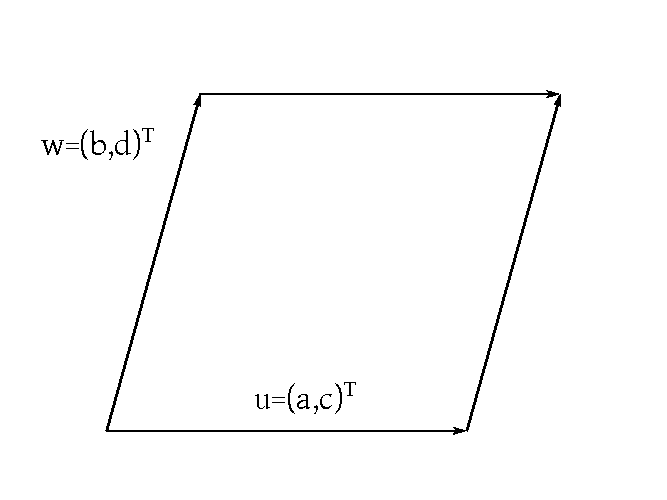
\includegraphics{img/01_geometric_interpretation_determinant.pdf}
      \caption{Geometric interpretation of determinants}
      \label{img:geo_det}
    \end{center}
  \end{figure}
  See Figure~\ref{img:geo_det}.
  The determinant $\det(v,w)$ is the area of the spanned parallelogram.
  We denote $F$ as the function returning the area of a geometric object.
\end{corollary}

\begin{proof}
  $\operatorname{area}(v,w)$ satisfies properties $(i)-(iii)$.

  Consider orthogonal $e_1$ and $e_2$.
  $F = 1 = \det(e_1, e_2)$. $\det(e_2, e_1) = -1$.

  The sign indicates the orientation of the area.
\end{proof}

By property~2, if $v=w$, then $F = 0$.
\index{Linear dependence}
By property~1,
\begin{enumerate}
  \item 
    If $v$ and $w$ are \emph{linear dependent}\footnote{Hence, one vector is a multiple of the other}, then
    \[ \lambda v + \mu w = 0 \qquad (\lambda, \mu) \neq (0, 0) \]
    Without loss of generality, $\mu \neq 0 \implies w = - \frac{\lambda}{\mu} \cdot v$.
  \item
    To show:
    \[ F(\lambda v, w) = \lambda \cdot F(v, w) \]
    \[ F(v + v', w) = F(v, w) + F(v', w) \]

    Let $\lambda \in \mathbb N$. We multiply the area $n$ times.
    \[ F(n \cdot v, w) = n \cdot F(v, w) \]
  \item
    \[ F\left(\frac1n \cdot v, w\right) = \frac1n F(v, w) \]
    follows from $F(\lambda v, w) = \lambda \cdot F(v, w)$, because $v = n \cdot (\frac1n v)$:
    \[ F\left(n \left(\frac1n v\right), w\right) = n \cdot F\left(\frac1n v, w\right) \]
  \item
    \begin{figure}[!h]
      \begin{center}
        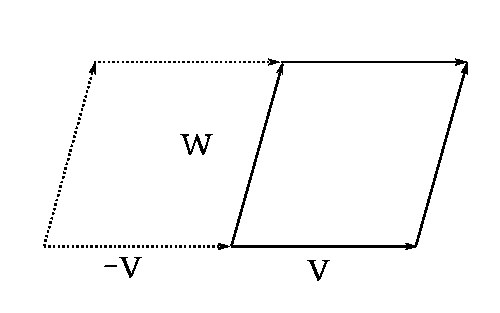
\includegraphics{img/02_continuity.pdf}
        \caption{The sign changes if the orientation changes}
        \label{img:continuity}
      \end{center}
    \end{figure}
    If we combine (2) and (3),
    \[ F\left(\frac mn v, w\right) = \frac mn F(v, w) \]
    See Figure~\ref{img:continuity}.
  \item
    By continuity, $F(\lambda v, w) = \lambda F(v, w) \forall \lambda \in \mathbb R_+$\footnote{By the way, how are real numbers defined?}.
    If the orientation changes, the sign changes. By this property, this actually holds for $\mathbb R$, not only $\mathbb R_+$.

    Analogously:
    \[ F(v, \lambda w) = \lambda F(v, w) \forall \lambda \in \mathbb R \forall v, w \in \mathbb R^2 \]
  \item
    To show: $F(v + v', w) = F(v, w) + F(v', w)$

    If $v$ and $w$ are linear independent, then $F(v + w, w) = F(v, w)$.
    In general, for a parallelogram of height $h$ and vector $w$, it holds that
    \[ F = \card{w} \cdot h \]
    The height of the parallelogram stays the same.
    \[ F(v, w) = F(v + w, w) \]
  \item 
    \[ F(\lambda v + \mu w, w) = \lambda F(v, w) \]
    \begin{description}
      \item[Case $\mu = 0$] Already shown, $F(\lambda v, w) = \lambda F(v, w) \forall \lambda \in \mathbb R$.
      \item[Case $\mu \neq 0$] $F(\lambda v + \mu w, w) = \frac1\mu F(\lambda v + \mu w, \mu w) = \frac1\mu F(\lambda v, \mu w) = F(\lambda v, w) = \lambda F(v, w)$
    \end{description}
  \item
    Let $v$ and $w$ be linear independent, then they define a basis of $\mathbb R^2$.
    \begin{align*}
      v_1 &= \lambda_1 v + \mu_1 w \\
      v_2 &= \lambda_2 v + \mu_2 w
    \end{align*}
    \begin{align*}
      \rightarrow F(v_1 + v_2, w)
        &= F(\lambda_1 v + \mu, w + \lambda_2 v + \mu_2 w, w) \\
        &= F((\lambda_1 + \lambda_2) v + (\mu_1 + \mu_2) w, w) \\
        &= F((\lambda_1 + \lambda_2) v, w) \\
        &= (\lambda_1 + \lambda_2) F(v, w) \\
        &= \lambda_1 F(v,w) + \lambda_2 F(v,w) \\
        &= F(\lambda_1 v, w) + F(\lambda_2 v, w) \\
        &= F(\lambda_1 v + \mu_1 w, w) + F(\lambda_2 v + \mu_2 w, w) \\
        &= F(v_1, w) + F(v_2, w)
    \end{align*}
    This shows that additivity is given.
\end{enumerate}

\subsection{Determinant form} % section 7.6

\begin{definition}
  \index{Determinant form}
  Let $V$ be an $n$-dimensional vector space over $\mathbb K$.
  A \emph{determinant form} is a map
  \[ \triangle: V^n \to \mathbb K \]
  \[ (a_1, \ldots, a_n) \mapsto \triangle (a_1, \ldots, a_n) \]
\end{definition}
Let $n=2$.
\[ \triangle: \left(\vectwo ac, \vectwo bd\right) \mapsto \begin{vmatrix} a & b \\ c & d \end{vmatrix} = ad - bc \]

\index{Multilinearity}
It satisfies the properties of \emph{multilinearity}:
\begin{enumerate}
  \item $\triangle(a_1, \dots, \lambda a_k, \dots, a_n) = \lambda \triangle(a_1, \dots, a_n)$
  \item $\triangle(a_1, \dots, a_k + v, \dots, a_n) = \triangle(a_1, \dots, a_k, \dots, a_n) + \triangle(a_1, \dots, a_{k-1}, v, a_{k+1}, \dots, a_n)$
\end{enumerate}
Multilinearity is given, if linearity is given in every component.
Hence, if $a_1, \dots, a_{k-1}, a_{k+1}, \dots, a_n$ are fixed, then
\[ V \to \mathbb K \]
\[ v \mapsto \triangle (a_1, \dots, a_{k-1}, v, a_{k+1}, \dots, a_n) \text{ linear} \]


Furthermore, it satisfies the following property:
\[ \triangle(a_1, \dots, a_n) = 0 \]
if $\exists k \neq l: a_k = a_l$.
If $\triangle \not\equiv 0$, then $\triangle$ is called \emph{non-trivial}.

\begin{corollary} % section 7.7
  \[ \triangle(a_1, \dots, a_k + \lambda a_i, \dots, a_n) = \triangle(a_1, \dots, a_k, \dots, a_n) \forall \lambda \in \mathbb K, \forall i \neq k \]
  \[ \triangle(a_1, \dots, a_i, \dots, a_j, \dots, a_n) = -\triangle(a_1, \dots, a_j, \dots, a_i, \dots, a_n) \]
\end{corollary}
\begin{proof}
  \begin{align*}
    \triangle(a_1, \dots, a_k + \lambda a_i, \dots, a_n)
      &= \triangle (a_1, \dots, a_k, \dots, a_n) + \triangle (a_1, \dots, a_{k-1}, \lambda a_i, a_{k+1}, \dots, a_n) \\
      &= \triangle (a_1, \dots, a_n) + \lambda \triangle (a_1, \dots, a_{k-1}, a_i, a_{k+1}, \dots, a_n) \\
      &= 0 \qquad \text{because $a_i$ occurs twice}
  \end{align*}
\end{proof}

\begin{align*}
  0 &= \triangle(a_1, \dots, a_i + a_j, \dots, a_i + a_j, \dots, a_n) \\
    &= \triangle(a_1, \dots, a_i, \dots, a_i, \dots, a_n) \\
    &+ \triangle(a_1, \dots, a_i, \dots, a_j, \dots, a_n) \\
    &+ \triangle(a_1, \dots, a_j, \dots, a_i, \dots, a_n) \\
    &+ \triangle(a_1, \dots, a_j, \dots, a_j, \dots, a_n)
\end{align*}
The first and last term are zero. Multilinearity is given:
\[ \lambda(a_1, \dots, \lambda a_k, \dots, a_n) = \lambda \triangle (a_1, \dots, a_n) \]
\[ \lambda(a_1, \dots, \lambda a_k + v, \dots, a_n) = \lambda \triangle (a_1, \dots, a_n) + \triangle (a_1, \dots, a_{k-1}, v, a_{k+1}, \dots, a_n) \]

\dateref{2018/03/07}

Determinant form: $\dim{V} = n$
\[ \triangle: V^n \to \mathbb K \]

\begin{enumerate}
  \item $\triangle(a_1, \dots, a_{k-1}, \lambda a_k, a_{k+1}, \ldots, a_n) = \lambda \triangle(a_1, \dots, a_n)$
  \item $\triangle(a_1, \dots, a_{k-1}, a_k + v, a_{k+1}, \dots, a_n = \triangle(a_1, \dots, a_k, \dots, a_n) + \triangle(a_1, \dots, v, \dots, a_n)$
  \item $\triangle(a_1, \dots, a_n) = 0$ if $\exists i \neq j: a_i = a_j$
\end{enumerate}
Multilinearity is given by the first two properties.

$\triangle \not\equiv 0$

Then the fourth property follows:
\begin{enumerate}
  \item[4] $\triangle(a_1, \dots, a_{k} + \lambda a_i, \dots, a_n) = \triangle(a_1, \dots, a_n) \forall i \neq k \forall \lambda \in \mathbb K$
  \item $\triangle(a_1, \dots, a_i, \dots, a_j, \dots, a_n) = -\triangle(a_1, \dots, a_j, \dots, a_i, \dots, a_n)$
\end{enumerate}

\begin{example}
  Let $n=2$, $V = \mathbb K^2$.

  \[ \triangle \left(\vectwo ac, \vectwo bd\right) = ad - bc = \det\begin{pmatrix} a & b \\ c & d \end{pmatrix} \]
\end{example}

\subsection{Permutations and transpositions}

\begin{definition} % 7.8
  A \emph{permutation} is a bijective map $\sigma: \set{1,\dots,n} \to \set{1,\dots,n}$.
  $\sigma_n$ is the set of all permutations.
  \[ \card{\sigma_n} = n! \]
\end{definition}

\index{Symmetric group}
\begin{remark} % 7.9
  $\sigma_n$ in regards of composition defines a group with neutral element $\operatorname{id}$
  and is called \emph{symmetric group}.
\end{remark}

\begin{remark} % 7.10
  For $n \geq 3$, it is non-commutative.
\end{remark}

\begin{example} % 7.11
  Permutations:
  \[ \begin{pmatrix} 1 & 2 & 3 & 4 \\ 4 & 1 & 3 & 2 \end{pmatrix} \circ \begin{pmatrix} 1 & 2 & 3 & 4 \\ 1 & 3 & 4 & 2 \end{pmatrix} = \begin{pmatrix} 1 & 2 & 3 & 4 \\ 4 & 3 & 2 & 1 \end{pmatrix} \]
  So, e.g. 2 is mapped to 3 (right side of $\circ$) and 3 is mapped to 3 (left side of $\circ$). Hence 2 is mapped to 3 (right-hand side of $=$).
  \[ \begin{pmatrix} 1 & 2 & 3 & 4 \\ 4 & 1 & 3 & 2 \end{pmatrix}^{-1} = \begin{pmatrix} 1 & 2 & 3 & 4 \\ 2 & 4 & 3 & 1 \end{pmatrix} \]
\end{example}

\begin{definition}
  A \emph{transposition} is a permutation exchanging exactly 2 elements.

  \[
    \tau_{ij} : \begin{cases}
      i \mapsto j \\
      j \mapsto i \\
      k \mapsto k \forall k \notin \set{i,j}
    \end{cases}
  \] \[
    \tau_{ij}^{-1} = \tau_{ij}
  \]
\end{definition}

\begin{remark}
  Every permutation $\sigma \in \sigma_n$ with $\sigma \neq \operatorname{id}$ can be denoted as product of transpositions.
\end{remark}

\begin{proof}
  \[ \sigma = \begin{pmatrix} 1 & 2 & \dots & n \\ \sigma(1) & \sigma(2) & \dots & \sigma(n) \end{pmatrix} \]
  Example:
  \[ \sigma = \begin{pmatrix} 1 & 2 & 3 & 4 & 5 & 6 & 7 \\ 1 & 3 & 5 & 4 & 7 & 6 & 2 \end{pmatrix} \]
\end{proof}

Find transpositions $\tau_1, \dots, \tau_k$ such that $\sigma = \tau_1 \circ \tau_2 \circ \dots \circ \tau_k$.

If $\sigma = \operatorname{id}$, then $k=0$.

If $\sigma \neq \operatorname{id}$,
\[ k_1 = \min\setdef{i}{\sigma(i) \neq i} \neq \emptyset \]
\[ \tau_1 = \tau_{k_1 \sigma(k_1)} \]
\[ \sigma_1 = \tau_i \circ \sigma \]
if $\sigma_i = \operatorname{id}$, then $\tau_1 \circ \sigma = \operatorname{id}$. Then $\sigma = \tau_1^{-1} = \tau_i$.
\[ k_2 = \min\setdef{i}{\sigma_i(i) \neq i} \]
\[ \tau_2 = \tau_{k_2 \sigma_1(k_2)} \]
\[ \sigma_2 = \tau_2 \circ \sigma_1 \]


\begin{example}
  Let $k_1 = 2$.
  \[ \tau_1 = \tau_{23} \]
  \begin{align*}
    \sigma_1 &= \tau_{23} \circ \begin{pmatrix} 1 & 2 & 3 & 4 & 5 & 6 & 7 \\ 1 & 3 & 5 & 4 & 7 & 6 & 2 \end{pmatrix} \\
      &= \begin{pmatrix} 1 & 2 & 3 & 4 & 5 & 6 & 7 \\ 1 & 2 & 5 & 4 & 7 & 6 & 3 \end{pmatrix}
  \end{align*}
  $k_2 = 3$.
  \[ \tau_2 = \tau_{35} \]
  \begin{align*}
    \sigma_2 = \tau_2 \circ \sigma_1 &= \begin{pmatrix} 1 & 2 & 3 & 4 & 5 & 6 & 7 \\ 1 & 2 & 3 & 4 & 7 & 6 & 5 \end{pmatrix}
  \end{align*}

  $k_3 = 5$.
  \[ T_3 = T_{57} \]
  \begin{align*}
    \sigma_3 = \tau_3 \circ \sigma_2 &= \begin{pmatrix} 1 & 2 & 3 & 4 & 5 & 6 & 7 \\ 1 & 2 & 3 & 4 & 5 & 6 & 7 \end{pmatrix} \\
      &= \operatorname{id}
  \end{align*}
  \[ \tau_3 \circ \tau_2 \circ \tau_1 \circ \sigma = \operatorname{id} \]
  \[ \implies \tau_2 \circ \tau_1 \circ \sigma = T_3^{-1} \circ \operatorname{id} = \tau_3 \]
  \[ \tau_1 \circ \sigma = \tau_2^{-1} \circ T_3 = \tau_2 \circ \tau_3 \]
  \[ \sigma = \tau_1 \circ \tau_2 \circ \tau_3 \]
  and so on and so forth.

  \[ \tau_k \]
  \[ \sigma_k = \tau_k \circ \tau_{k-1} \circ \dots \circ \tau_{i} \circ \sigma = \operatorname{id} \]
  \[ \implies \sigma = \tau_1 \circ \tau_2 \circ \dots \circ \tau_k \]
\end{example}

\begin{remark}
  This decomposition is not unique.
\end{remark}

\index{Malposition}
\index{Signature of $\pi$}
\begin{definition} % 7.14
  Let $\pi \in \sigma_n$ be a permutation.
  A \emph{malposition} (dt. \foreignlanguage{german}{Fehlstand}) of $\pi$ is a pair $(i,j)$ such that $i < j$ and $\pi(i) > \pi(j)$.
  \[ f_\pi \coloneqq \card{\setdef{(i,j)}{(i,j) \text{ is malposition of } \pi}} \]
  \[ \sign(\pi) \coloneqq (-1)^{f_\pi} \eqqcolon (-1)^\pi \]
  is called \emph{signature of $\pi$}
\end{definition}

\begin{example} % 7.15
  \[ \pi = \begin{pmatrix} 1 & 2 & 3 & 4 & 5 & 6 & 7 \\ 1 & 3 & 5 & 4 & 7 & 6 & 2 \end{pmatrix} \]
  Malpositions:
  \[ \set{(2,7), (3,4), (3,7), (5,6), (5,7), (4,7), (6,7)} \]
  \[ 2 < 7 \]
  \[ \pi(2) - 3 > 2 = \pi(7) \]
  \[ f_\pi = 7 \]
\end{example}

\begin{theorem}
  \[ \sign(\pi) = \prod_{\substack{i,j \\ i < j}} \frac{\pi(j) - \pi(i)}{j-i} \]
  \begin{itemize}
    \item ${n \choose 2}$ factors
    \item for transposition, $\sign\tau = -1$.
  \end{itemize}
\end{theorem}

\begin{proof}
  \[ \prod_{i<j} \frac{\pi(j) - \pi(i)}{j-i} = \frac{\prod_{i<j} (\pi(j) - \pi(i))}{\prod_{i<j} (j-i)} \]
  $\pi$ is bijective in $\set{1, \dots, n}$
  Hence, every difference $j - i$ occurs exactly one time in the enumerator and the denomiator with sign $\pm 1$
  depending on whether $(i,j)$ is a malposition or not.
  \[ \sign(\pi(j) - \pi(i)) = \begin{cases}
    +1 & \pi(j) > \pi(i) \\
    -1 & \pi(j) < \pi(i) \text{ hence malposition}
  \end{cases} \]
\end{proof}

\begin{example}
  \[ \pi = \begin{pmatrix} 1 & 2 & 3 & 4 & 5 & 6 & 7 \\ 1 & 3 & 5 & 4 & 7 & 6 & 2 \end{pmatrix} \]
  Malposition:
  \[ \set{(2,7), (3,4), (3,7), (5,6), (5,7), (4,7), (6,7)} \]
  \[ 2 < 7 \]
  \[ \pi(2) - 3 > 2 = \pi(7) \]
  \[ f_\pi = 7 \]

  \[
    \frac{\prod_{i<j} (\pi(j) - \pi(i))}{\pi_{i<j} (j-i)} = \frac{\prod_{i<j} (j-i) \cdot (-1)^{f_\pi}}{\prod_{i<j} (j-i)} = \sign{\pi}
  \]

  \[ \pi = \begin{pmatrix} 1 & 2 & 3 \\ 3 & 2 & 1 \end{pmatrix} \]
  \begin{align*}
    \prod_{i<j} \frac{\pi(j) - \pi(i)}{j-i}
      &= \frac{\pi(2) - \pi(1)}{2 - 1} \cdot \frac{\pi(3) - \pi(1)}{3-1} \cdot \frac{\pi(3) - \pi(2)}{3-2} \\
      &= \frac{(2-3) \cdot (1-3) \cdot (1 - 2)}{(2-1) (3-1) (3-2)} \\
      &= (-1)^3 = -1
  \end{align*}

  Malpositions:
  \begin{enumerate}
    \item $(1,2)$
    \item $(1,3)$
    \item $(2,3)$
  \end{enumerate}

  Transposition: Let $k < \tau(k)$.
  \[
    \tau = \left\{\begin{array}{ccccccccccc}
      1 & 2 & \ldots & k-1 & k       & k+1 & \ldots & \tau(k) & \tau(k+1) & \ldots & n \\
      1 & 2 & \ldots & k-1 & \tau(k) & k+1 & \ldots & k       & \tau(k+1) & \ldots & n
    \end{array}\right\}
  \]
  Malpositions (denoted $F_\tau$):
  \[
    F_\tau = \begin{cases}
      & (k, k+1), \dots, (k, \tau(k)) \\
      & (k+1, \tau(k)), (k+2, \tau(k)), \dots, (\tau(k)-1, \tau(k))
    \end{cases}
  \]

  Let us count on a specific example:
  \[ \begin{pmatrix}
    1 & 2 & 3 & 4 & 5 & 6 & 7 \\
    1 & 2 & 6 & 4 & 5 & 3 & 7
  \end{pmatrix} \]

  \[
    \begin{cases}
      & (3,4), (3,5), (3,6) \\
      & (4,6), (5,6)
    \end{cases}
  \]

  \[ \card{F_\tau} = (\tau(k) - k) + \left((\tau(k) - 1) - k\right) = 2\tau(k) - 2k - 1 = 2(\tau(k) - k) - 1 \text{ even} \]
\end{example}

\begin{theorem} % 7.17
  \begin{enumerate}
    \item $\sign(\operatorname{id}) = 1$
    \item $\sign(\pi \circ \sigma) = \sign(\pi) \circ \sign(\sigma)$ \\
      Hence, $\sign\sigma_n \to \set{\pm 1}$ is a homomorphism.

      $(\set{+1, -1}, \cdot)$ is a group $\stackrel{\sim}{=} (\mathbb Z_2, +)$
      \[ +1 \to [0]_2 \]
      \[ -1 \to [1]_2 \]
    \item $\sign(\pi^{-1}) = \sign(\pi)$
  \end{enumerate}
\end{theorem}

\begin{proof}
  \begin{enumerate}
    \item obvious, because there are no malpositions
    \item
      \begin{align*}
        \sign(\pi \circ \sigma) &= \prod_{i<j} \frac{(\pi \circ \sigma(j) - \pi \circ \sigma(i))}{j-i} \prod_{i<j} \frac{\sigma(j) - \sigma(i)}{\sigma(j) - \sigma(i)}
        \intertext{because of bijectivity}
          &= \underbrace{\prod_{i<j} \frac{\pi(\sigma(j)) - \pi(\sigma(i))}{\sigma(j) - \sigma(i)}}_{\sign\pi} \cdot \underbrace{\prod_{i<j} \frac{\sigma(j) - \sigma(i)}{j - i}}_{\sign\pi}
      \end{align*}
    \item Homomorphism
      \[ \sign(\pi^{-1}) = \sign(\pi)^{-1} = \sign(\pi) \]
  \end{enumerate}
\end{proof}

\begin{remark}
  Recall that the kernel of a homormophism defines a subgroup.
\end{remark}

\index{Alternating group}
\begin{corollary}
  \begin{enumerate}
    \item If $\pi = \tau_1 \circ \dots \circ \tau_k$ is a product of transpositions, then $\sign(\pi) = (-1)^k$
    \item $\mathfrak a_n = \setdef{\pi \in \sigma_n}{\sign(\pi) = +1} = \operatorname{ker}(\sign: \sigma_n \to \set{\pm 1})$
      is a subgroup of $\sigma_n$, the so-called \emph{alternating group}
      \[ \card{\mathfrak a_n} = \frac{n!}{2} \]
  \end{enumerate}
\end{corollary}

\begin{corollary} % 7.19
  \label{cor:719}
  \[ \dim V = n \]
  \[ \triangle: V^n \to \mathbb K \qquad \text{ determinant form} \]
  then it holds that $\forall \sigma \in \sigma_n: \triangle(a_{\sigma(1)}, \dots, a_{\sigma(n)}) = \sign(a) \cdot \triangle(a_1, \dots, a_n)$
\end{corollary}

\begin{proof}
  If $\sigma = \tau$ is a transposition, the fourth property:
  \[ \triangle(a_{\tau(1)}, \dots, a_{\tau(n)}) = -\triangle(a_1, \dots, a_n) \]
  and $\sign(\tau) = -1$.

  The general case: $\sigma = \tau_1 \circ \dots \circ \tau_k$ and $\sigma = \tau_1 \circ \sigma_1$.

  \begin{align*}
    \triangle(a_{\sigma(1)}, \dots, a_{\sigma(n)}) &= \triangle(a_{\tau_1(\sigma_1(1))}, \dots, a_{\tau_1(\sigma_1(n))}) \\
      &= -\triangle(a_{\sigma_1(1), \dots, a_{\sigma_1(n)}}) \\
    \intertext{$\sigma_1 = \tau_2 \circ \sigma_2$}
      &= \text{ and so on and so forth} \\
      &= (-1)^2 \triangle(a_{\sigma_2(1)}, \dots, a_{\sigma_2(n)}) \\
      &= (-1)^k \triangle (a_1, \dots, a_n) \\
      &= \sign\sigma \triangle(a_1, \dots, a_n)
  \end{align*}
\end{proof}

\subsection{Leibniz formula for determinants}

\index{Determinant}
\begin{definition} % 7.20
  \label{det}
  Let $\dim V = n$. Let $B = (b_1, \dots, b_n)$ be a basis of $V$. $a_1, \dots, a_n \in V$ with coordinates
  \[
    \psi_B(a_j) = \begin{pmatrix} a_{1j} \\ a_{2j} \\ \vdots \\ a_{nj} \end{pmatrix}
    \qquad
    A \coloneqq \begin{bmatrix} a_{11} & \dots & a_{1n} \\ \vdots &  & \vdots \\ a_{n1} & \dots & a_{nn} \end{bmatrix}
  \]
  Then $\triangle(a_1, \dots, a_n) = \det(A) \cdot \triangle(b_1, \dots, b_n)$
  where
  \[ \det(A) \coloneqq \sum_{\pi \in \sigma_n} \sign(\pi) a_{1\pi(1)} a_{2 \pi(2)} \dots a_{n\pi(n)} \]
  is called \emph{determinant of $A$}

  This formula was discovered by Leibniz.
\end{definition}

\begin{example}
  Consider $n=2$.
  \[
    \begin{vmatrix}
      a_{11} & a_{12} \\
      a_{21} & a_{22}
    \end{vmatrix} = \underbrace{a_{11} a_{22}}_{\pi = \operatorname{id}} - \underbrace{a_{12} a_{21}}_{\pi = \begin{pmatrix} 1 & 2 \\ 2 & 1 \end{pmatrix}}
  \]
\end{example}

\begin{proof}
  \[ a_j = \sum_{i=1}^n a_{ij} b_2 \]
  \begin{align*}
    \triangle(a_1, \dots, a_n) &= \triangle\left(\sum_{i_1 = 1}^n a_{i_1,1} b_{i_1}, \sum_{i_2 = 1}^n a_{i_2,2} b_{i_2}, \dots, \sum_{i_n = 1}^n a_{i_n, n} b_{i_n}\right) \\
    \intertext{because it is multilinear}
      &= \sum_{i_1 = 1}^n \sum_{i_2=1}^n \dots \sum_{i_n=1}^n a_{i+1,1} a_{i_2,2} \dots a_{i_n,n} \cdot \triangle(b_{i_1}, b_{i_2}, \dots, b_{i_n})
  \end{align*}
  where $\triangle = 0$ is two indices equate.
  \[ \implies i_1,\dots,i_n \text{ are all difference } \in \set{1,\dots,n} \]
  \[ \implies \text{every occurs exactly once} \]
  \[ i_1,\dots,i_n \text{ is permutation of } 1,\dots,n \]
  \[ \exists \sigma \in \sigma_n: i_1 = \sigma(1), \dots, i_n = \sigma(n) \]
  \begin{align*}
    &= \sum_{\sigma \in \sigma_n} a_{\sigma(1) 1} a_{\sigma(2) 2} \dots a_{\sigma(n) n} \underbrace{\triangle(b_{\sigma(1)} \dots b_{\sigma(n)})}_{\sign\sigma \triangle(b_1, \dots, b_n) \text{ because of Corollary~\ref{cor:719}}} \\
    &= \sum_{\pi \in \sigma_n} a_{1 \pi(1)} \dots a_{n \pi(n)} \cdot \sign(\pi) \triangle(b_1, \dots, b_n)
  \end{align*}
\end{proof}

\begin{corollary}
  A determinant form is uniquely defined by the value $\triangle(b_1, \dots, b_n)$ on a basis.

  Especially, $\triangle \not\equiv 0 \iff \triangle(b_1,\dots,b_n) \neq 0$ [for any basis] $\iff \triangle(b_1,\dots,b_n) \neq 0$ [for every basis].

  Assume $\triangle(b_1,\dots,b_n) = 0$ for any basis.
  Every other basis can be expressed by $b_1,\dots,b_n$ and the formula gives $\triangle(a_1,\dots,a_n) = 0 \forall a_1,\dots,a_n$.
\end{corollary}

\dateref{2018/03/12}

\begin{theorem} % 7.21
  \[ \triangle \text{ non-trivial } \iff \triangle(b_1, \dots, b_n) \neq 0 \text{ for every basis} \]
\end{theorem}

\begin{theorem} % 7.20
  \label{thm720}
  Define determinant of matrix $A$.

  \[ \triangle(a_1, \dots, a_n) = \triangle(b_1, \dots, b_n) \cdot \det{A} \]
  if $a_j = \sum_{i=1}^n a_{ij} b_i$.
  Hence
  \[ \begin{pmatrix} a_{1j} \\ a_{ij} \\ \vdots \\ a_{nj} \end{pmatrix} = \Phi_{B}(a_j) \]
\end{theorem}

\begin{theorem} % 7.22
  \label{theorem722}
  Inverse of Theorem~\ref{thm720}.
  Given basis $B = (b_1, \dots, b_n)$.
  \[ \triangle(a_1, \dots, a_n) \coloneqq \det\left[\Phi_B(a_1), \dots, \Phi_B(a_n)\right] \]
  defines a non-trivial determinant form such that $\triangle(b_1, \dots, b_n) = 1$
\end{theorem}

\begin{corollary} % Folgerung 7.23
  \label{folgerung723}
  Let $\triangle$ be a non-trivial determinant form.
  Then $v_1, \dots, v_n$ is linearly independent.
  \[ \iff \triangle(v_1, \dots, v_n) \neq 0 \]

  Direction $\Rightarrow$: Immediate, because $v_1, \dots, v_n$ is a basis.

  Direction $\Leftarrow$: Assume $v_1, \dots, v_n$ is linearly independent.
  Without loss of generality, $v_n = \sum_{k=1}^{n-1} \lambda_k v_k$.
  \begin{align*}
    \triangle(v_1, \dots, v_n) &= \triangle(v_1, \dots, v_{n-1}, \sum_{k=1}^{n-1} \lambda_n v_k) \\
      &= \sum_{k=1}^{n-1} \lambda_k \triangle \underbrace{(v_1, \dots, v_{n-1}, v_k)}_{=0 \text{ because $v_k$ occurs twice}} \\
      &= 0
  \end{align*}
\end{corollary}

\begin{remark}[Summary]
  \begin{enumerate}
    \item The determinant form defines a 1-dimensional vector space.
    \item There exists a non-trivial determinant form. Given a basis $b_1, \dots, b_n$
      \[ \triangle(b_1, \dots, b_n) = \mathbf 1 \]
      By Theorem~\ref{theorem722}, $\triangle(a_1, \dots, a_n) = \det(\Phi_B(a_1), \dots, \Phi_B(a_n))$.
  \end{enumerate}
\end{remark}

\begin{proof}[Proof of Theorem~\ref{theorem722}]
  \begin{enumerate}
    \item
      \begin{align*}
        \triangle(a_1, \dots, \lambda a_k, \dots, a_n)
          &= \sum_{\pi \in \sigma_n} (-1)^{\pi} a_{\pi(1)1} \lambda a_{\pi(k) k} a_{\pi(n) n} \\
          &= \lambda \cdot \sum_{\pi \in \sigma_n} (-1)^\pi a_{\pi(1) 1} \dots a_{\pi(n) n} \\
          &= \lambda \cdot \triangle(a_1, \dots, a_n)
      \end{align*}
    \item
      \begin{align*}
        \triangle(a_1, \dots, a_k + v, \dots, a_n)
          &= \sum_{\pi \in \sigma_n} (-1)^\pi a_{\pi(1) 1} \dots (a_{\pi(k) k} + v_{\pi(k)}) \cdot a_{\pi(n)} n \\
          &= \sum_{\pi \in \sigma_n} (-1)^\pi a_{\pi(1) 1} \dots a_{\pi(k) k} \dots a_{\pi(n) n} \\
    &+ \sum_{\pi \in \sigma_n} (-1)^\pi a_{\pi(1) 1} \dots v_{\pi(k) k} \dots a_{\pi(n) n} \\
          &= \triangle(a_1, \dots, a_k, \dots, a_n) + \triangle(a_1, \dots, v, \dots, a_n)
      \end{align*}
      This proves multilinearity.
    \item
      Let $a_k = a_l$, $a_{ik} = a_{il} \forall i = 1, \dots, n$.
      Without loss of generality, $k < l$.
      \[ \triangle(a_1, \dots, a_k) = \sum_{\pi \in \sigma_n} (-1)^\pi a_{\pi(1) 1} \dots a_{\pi(k) k} \dots a_{\pi(l) l} \dots a_{\pi(n) n} \]
      \[ \tau \cdot \pi = (\text{reference *}) \]
      Let $\tau = \tau_{kl}$, exchange of $k$ and $l$.
      \begin{claim}
        \[ \sigma_n = \underbrace{\mathcal A_n}_{\substack{\text{alternating group} \\ = \setdef{\pi}{\sign(\pi) = +1}}} \cup \underbrace{\mathcal A_{n} \cdot \tau}_{= \setdef{\pi \circ \tau}{\pi \in \mathcal A_n}} \]
      \end{claim}
      \begin{proof}
        Direction $\Leftarrow$.
        Let $\sign(\pi) = -1$.
        \[ \Rightarrow \pi = (\pi \circ \underbrace{\tau) \circ \tau}_{= \operatorname{id}} \]
        $\sigma = \pi \circ \tau$ has $\sign(\sigma) = \sign(\pi \circ \tau) = \sign(\pi) \cdot \sign(\tau) = (-1) \cdot (-1) = 1$.
        \[ \sigma \in \mathcal A_n \text{ and } \pi = \sigma \circ \tau \]
        \begin{align*}
          \text{reference *} &= \sum_{\pi \in \mathcal A_n} \underbrace{(-1)^\pi}_{=+1} a_{\pi(1) 1} \dots a_{\pi(n) n} \\
            &+ \sum_{\substack{\pi \in \mathcal A_n \tau \\ \pi = \sigma \circ \tau}} \underbrace{(-1)^{\sign(\pi)}}_{= -1} a_{\pi(1) 1} \cdot a_{\pi(n) n} \\
            &= \sum_{\pi \in \mathcal A_n} a_{\pi(1) 1} \dots a_{\pi(n) n} - \sum_{\sigma \in A_n} \underbrace{a_{\sigma \circ \tau(1) 1} \dots a_{\sigma \circ \tau(k) 2} \dots a_{\sigma \circ \tau(l) l} \dots a_{\sigma \circ \tau(n) n}}_{a_{\sigma(1) 1} \dots \underbrace{a_{\sigma(l) k}}_{=a_{\sigma(l) l}} \dots \underbrace{a_{\sigma(k) l}}_{= a_{\sigma(k) k}} \dots a_{\sigma(n) n}} = 0
        \end{align*}
      \end{proof}
  \end{enumerate}
\end{proof}

This previous part, beginning with the reference from 2018/03/12, was actually added on 2018/03/14, because we skipped it by accident.

\[ \triangle(a_1, \dots, a_n) \]
Determinant form $\iff$
\begin{description}
  \item[multilinear] $\triangle(a_1, \dots, \lambda a_k + \mu a_k', \dots, a_n) = \lambda \triangle(a_1, \dots, a_k, \dots, a_n) + \mu \triangle(a_1, \dots, a_k, \dots, a_n)$
  \item[anti-symmetrical] $\triangle(a_1, \dots, a_k, \dots, a_l, \dots, a_n) = -\triangle(a_1, \dots, a_l, \dots, a_k, \dots, a_n)$
\end{description}

\[ \triangle (a_{\pi(1)}, \dots, a_{\pi(n)}) = (-1)^\pi \triangle(a_1,\dots,a_n) \]
where $(-1)^\pi \coloneqq \sign(\pi) = (-1)^{(F(\pi))}$
\[ F(\pi) = \setdef{(i,j)}{i < j \land \pi(i) > \pi(j)} \]
\[ \sign(\pi \circ \sigma) = \sign(\pi) \cdot \sign(\pi) \cdot \sign(\sigma) \]

Basis $b_1,\dots,b_n$.
\[ \triangle(\sum_{i=1}^n a_{i1} b_i, \dots, \sum_{i=1}^n a_{in} b_i) = \det{A} \cdot \triangle(b_1, \dots, b_n) \]
\[ \det(A) = \sum_{\pi \in \sigma_n} (-1)^\pi  a_{1\pi(1)} \dots a_{n\pi(n)} = \sum_{\pi \in \sigma_n} (-1)^\pi a_{\pi(1) 1} \dots a_{\pi(n) n} \]

\begin{lemma} % 7.25
  Let $V, W$ be vector spaces over $\mathbb K$ with $\dim{V} = \dim{W} = n$.
  Let $\triangle: W^n \to \mathbb K$ be a determinant form and $f: V \to W$ linear.
  \[ V \xrightarrow{f} W \]
  \[ V^n \xrightarrow{f^{(n)}} W^n \xrightarrow{\triangle} \mathbb K \]
  \[ (v_1, \dots, v_n) \mapsto (f(v_1), \dots, f(v_n)) \]

  \[ \implies \triangle^f: V^n \to \mathbb K \]
  \[ \triangle^f(v_1, \dots, v_n) = \triangle(f(v_1), \dots, f(v_n)) \]
  is a determinant form on $V$.
\end{lemma}

\begin{proof}
  \begin{enumerate}
    \item Multilinear
      \begin{align*}
        &\triangle^f (v_1, \dots, \lambda v_k + \mu v_k', \dots, v_n) \\
        &= \triangle (f(v_1), \dots, f(\lambda v_k + \mu v_k'), \dots, f(v_n)) \\
        &= \triangle(f(k), \dots, \lambda f(v_k) + \mu f(v_k'), \dots, f(v_k)) \\
        &= \lambda \triangle (f(v_1), \dots, f(v_k), \dots, f(v_n)) + \mu \triangle(f(v_1), \dots, f(v_k'), \dots, f(v_n)) \\
        &= \lambda \triangle^f(v_1, \dots, v_k, \dots, v_n) + \mu \triangle^f (v_1, \dots, v_k', \dots, v_n)
      \end{align*}
  \end{enumerate}
\end{proof}

\begin{corollary} % Folgerung 7.26
  \label{cor726}
  Let $V = W$, $\triangle: V^n \to \mathbb K$ determinant form.
  \[ f: V \to V \text{ linear} \]
  \[ \implies \triangle^f \text{ is determinant form} \]
  Because there is (except for one factor) only one determinant form:
  \[ \exists C_f \in \mathbb K: \triangle^f(v_1, \dots, v_n) = C_f \cdot \triangle(v_1, \dots, v_n) \forall v_1,\dots,v_n \in V \]
  \[ \det(f) \coloneqq C_f \text{ is called \emph{determinant} on } f \]
\end{corollary}

\begin{proof}
  Let $\triangle_1$, $\triangle_2$ be two determinant forms.
  \[ \triangle_1 (v_1, \dots, v_n) = \det{A} \cdot \triangle_1(b_1, \dots, b_n) \]
  \[ \triangle_2 (v_1, \dots, v_n) = \det{A} \cdot \triangle_2(b_1, \dots, b_n) \]
  if $b_1, \dots, b_n$ is basis and
  \[ v_j = \sum_{i=1}^n a_{ij} b_i \]
  \[ \implies \triangle_2(v_1, \dots, v_n) = \frac{\triangle_2(b_1, \dots, b_n)}{\triangle_1(b_1, \dots, b_n)} \cdot \triangle_1(v_1, \dots, v_n) \]
  \[ \implies C_f = \frac{\triangle^f(b_1, \dots, b_n)}{\triangle (b_1, \dots, b_n)} = \det(f) \]
\end{proof}

\subsection{On determinants, invertibility and linear independence}

\begin{corollary} % Folgerung 7.27
  $B = (b_1, \dots, b_n)$ is basis of $V$.
  $\phi_B^B(f)$ is matrix representation of $f$ and $\det(f) = \det\phi_B^B(f)$
  (LHS by Corollary~\ref{cor726}, RHS by Definition~\ref{det} $\sum_{\pi} (-1)^\pi \dots$)
\end{corollary}

\begin{proof}
  \[ \det(f) = \frac{\triangle(f(b_1)), \dots, \triangle(f(b_n)))}{\triangle (b_1, \dots, b_n)} \]
  \begin{align*}
    f(b_j) &= \sum_{i=1}^n \phi_B(f(b_i))_i \cdot b_i \\
         &= \sum_{i=1}^n \left(\phi_B^B(f)\right)_{ij} b_i
  \end{align*}
  with $\phi_B^B(f)_{ij} = \phi_B(f(b_j))_i$.
  \begin{align*}
    \det{f} &= \frac{\det{\phi_B^B(f) \cdot \triangle(b_1, \dots, b_n)}}{\triangle(b_1, \dots, b_n)}
  \end{align*}
\end{proof}

\begin{theorem} % 7.28
  $f: V \to V$ is invertible $\iff \det(f) \neq 0$.
\end{theorem}
\begin{proof}
  Let $\triangle$ be a non-trivial determinant form.
  \[ B = (b_1, \dots, b_n) \text{ is a basis } \implies \triangle(b_1, \dots, b_n) \neq 0 \]
  \[ \det(f) = \frac{\triangle(f(b_1), \dots, f(b_n))}{\triangle(b_1, \dots, b_n)} \]
  $(f(b_1), \dots, f(b_n))$ is basis $\iff f$ is invertible.

  If $f$ is invertible, then $(f(b_1), \dots, f(b_n))$ is basis.
  \[ \implies \triangle (f(b_1), \dots, f(b_n)) \neq 0 \implies \det(f) \neq 0 \]

  If $f$ is not invertible, then
  \[ \implies f(b_1) \dots f(b_n) \text{ is linear dependent} \]
  \[ \exists k: f(b_k) = \sum_{i\neq k} \lambda_i f(b_i) \]
  Without loss of generality: $k = n$
  \begin{align*}
    \triangle(f(b_1), \dots, f(b_n)) &= \triangle(f(b_1), \dots, f(b_{n-1}), \sum_{i=1}^{n-1} \lambda_i f(b_i)) \\
      &= \sum_{i=1}^n \lambda_i \triangle(\underbrace{f(b_1), \dots, f(b_{n-1})}_{=0 \forall i \in \set{1,\dots,n-1}}, f(b_i)) \\
      &= 0
  \end{align*}
\end{proof}

\begin{corollary}
  For a matrix $A \in \mathbb K^{n\times n}$ it holds that $\det{A} \neq 0 \iff$ A has full rank.
\end{corollary}

\begin{theorem} % 7.29
  $f, g: V \to V$ linear.
  \[ \implies \det(f \circ g) = \det(f) \cdot \det(g) \]
  for a matrix: $\det(A \cdot B) = \det(A) \cdot \det(B)$
\end{theorem}

\begin{proof}
  Case 1: $f$ and $g$ are invertible.
  \[ \det(f) = \frac{\triangle (f(b_1), \dots, f(b_n))}{\triangle(b_1, \dots, b_n)} \]
  for arbitrary bases $(b_1, \dots, b_n)$ of $V$.
  \begin{align*}
    \det(f \circ g) &= \frac{\triangle(f(g(b_1)), \dots, f(g(b_n)))}{\triangle(b_1, \dots, b_n)} \cdot \frac{\triangle(g(b_1), \dots, g(b_n))}{\triangle(g(b_1), \dots, g(b_n))} \\
      &= \frac{\triangle(f(g(b_1)), \dots, f(g(b_n)))}{\underbrace{\triangle(g(b_1), \dots, g(b_n))}_{0 \neq \det(f)}} \cdot \underbrace{\frac{\triangle(g(b_1), \dots, g(b_n))}{\triangle(b_1, \dots, b_n)}}_{\det(g) \neq 0}
  \end{align*}
  $g$ invertible
  \[ \implies g(b_1), \dots, g(b_n) \text{ is basis} \]
\end{proof}

\begin{claim}
  $f \circ g$ invertible $\iff$ $f$ invertible and $g$ invertible.

  $f \circ g$ invertible $\implies$ $f \circ g$ surjective $\implies f$ surjective $\implies$ ($\dim{V} < \infty$) $f$ is bijective.

  $f \circ g$ invertible $\implies$ $f \circ g$ injective $\implies$ $g$ injective $\implies$ $g$ bijective.

  Case 2: $\neg(f \text{ bijective} \land g \text{ bijective}) \implies f \circ g \text{ not bijective}$

  $f$ is not bijective or $g$ is not bijective.
  \[ \det(f) = 0 \lor \det(g) = 0 \iff \det(f) \circ \det(g) = 0 = \det(f \circ g) \]
\end{claim}

\begin{corollary} % Korollar 7.30
  \label{cor730}
  For $A, B \in \mathbb K^{n\times n}$ it holds that
  \begin{enumerate}
    \item $\det(A \cdot B) = \det(A) \cdot \det(B)$
    \item $\det(A^{-1}) = \frac{1}{\det(A)}$ if invertible
    \item $\det(A) = 0 \iff \rank(A) < n$
    \item $\det(A^t) = \det(A)$
  \end{enumerate}
\end{corollary}

\begin{proof}[Proof of Corollary~\ref{cor730}]
  \begin{enumerate}
    \item $\det(A \cdot B) = \det(f_A \circ f_B) = \det(f_A) \cdot \det(f_B) = \det(A) \cdot \det(B)$
    \item $A \cdot A^{-1} = I$ and $1 = \det(A \cdot A^{-1}) = \det(A) \cdot \det(A^{-1})$
  \end{enumerate}
  \begin{remark}[From the practicals]
    \[ \det(A) = \det(f_A) \]
    Shown so far:
    \[ \det{f} = \det\left(\phi_B^B(f)\right) \]
    \[ A = \phi_B^B\left(f_A\right) \]
    for $B = (e_1, \dots, e_n)$
  \end{remark}
\end{proof}

\begin{proof}[Direct proof of Corollary~\ref{cor730} (1)]
  \[ A = \begin{bmatrix} s_1 & \dots & s_n \\ \vdots &  & \vdots \end{bmatrix} \]
  $s_1$ are column vectors of $A$.
  Let $\triangle$ be the uniquely defined determinant form by $\triangle(e_1, \dots, e_n) = 1$.
  \[
    A \cdot B
    = \begin{bmatrix} s_1 & \dots & s_n \\ \vdots &  & \vdots \end{bmatrix} \cdot \begin{bmatrix} b_{11} & b_{12} & \dots & b_{1n} \\ \vdots & & & \vdots \\ b_{n1} & & & b_{nn} \end{bmatrix}
  \] \[
    = \begin{bmatrix} s_1 b_{11} + s_2 b_{21} + \dots + s_n b_{n1} & s_1 b_{12} + s_2 b_{22} + \dots + s_n b_{n2} & \dots & s_1 b_{1n} + s_2 b_{2n} + \dots + s_n b_{nn} \\
    \vdots & \vdots &  & \vdots \end{bmatrix}
  \] \[
    \det(A \cdot B) = \frac{\triangle(s_1(A \cdot B), \dots, s_n(A \cdot B))}{\triangle (e_1, \dots, e_n)}
      = \triangle\left(\sum_{i_1=1}^n s_{i_1} b_{i_1 1}, \sum_{i_2=1}^n s_{i_2} b_{i_2 2}, \dots, \sum_{i_n=1}^n s_{i_n} b_{i_n n}\right)
  \] \[
    = \sum_{i_1=1}^n \dots \sum_{i_n=1}^n b_{i_1 1} b_{i_2 2} \dots b_{i_n n} \underbrace{\triangle(s_{i1}, \dots, s_{in}}_{=0}
  \]
  if one index occurs twice. It suffices to consider $\sum_{i_1,\dots,i_n}$ such that all $ij$ are difference.
  If all are difference, then all occur exactly once. Hence,
  $i_1,\dots,i_n$ is permutation of $1, \dots, n$.
  \begin{align*}
    &= \sum_{\pi \in \sigma_n} b_{\pi(1) 1} \dots b_{\pi(n) n} \triangle(s_{\pi(1)} \dots s_{\pi(n)}) \\
    &= \sum_{\pi \in \sigma_n} \underbrace{(-1)^\pi b_{\pi(1) 1} \dots b_{\pi(n) n}}_{\det{B}} \underbrace{\triangle(s_1, \dots, s_n)}_{= \det(A)} = \det(B) \cdot \det(A)
  \end{align*}
\end{proof}

\begin{proof}[Proof of Corollary~\ref{cor730} (4)]
  \begin{align*}
    \det(A^t) &= \sum_{\pi \in \sigma_n} (-1)^\pi (A^t)_{\pi(1) 1} \dots (A^t)_{\pi(n) n} \\
      &= \sum_{\pi \in \sigma_n} (-1)^\pi a_{1 \pi(1)} \dots a_{n \pi(n)}
  \end{align*}

  \begin{remark}
    \[ \sigma_n \to \sigma_n \]
    \[ \pi \mapsto \pi^{-1} \]
    is bijective.
    \[ \text{injective:} \pi^{-1} = \sigma^{-1} \implies \pi = \sigma \]
    \[ \text{surjective:} \pi = (\pi^{-1})^{-1} \]
  \end{remark}

  \[ = \sum_{\pi \in \sigma_n} (-1)^{\pi^{-1}} a_{1 \pi^{-1}(1)} \dots a_{n \pi^{-1}(n)} \]
  Every index $i$ occurs once on the left side and once on the right side. i occurs right
  \[ \pi^{-1}(j) = i  \iff  j = \pi(i) \]

  \[ = \sum_{\pi \in \sigma_n} (-1)^\pi a_{\pi(1) 1} \dots a_{\pi(n) n} \]

  \[ \sign(\pi \circ \pi^{-1}) = 1 \]
  \[ = \sign(\pi) \cdot \sign(\pi^{-1}) \]

  \begin{remark}[A small exercise]
    \[ \det(A) = \det(f_A) \]
    \[
      \prod_{j=1}^n a_{j, \pi^{-1}(j)}
      = \prod_{i=1}^n a_{\pi(i), \pi^{-1}(\pi(i))}
      = \prod_{i=1}^n a_{\pi(i), i}
    \] \[
      j = \pi(i)
    \]
  \end{remark}
\end{proof}

\index{Permanent of a square matrix}
\begin{definition}
  \[ \perm(A) \coloneqq \sum_{\pi \in \sigma_n} a_{\pi(1) 1} \dots a_{\pi(n) n} \]
  is called \emph{permanent of $A$}.

  Open problem: for which matrix does $\perm(A) = 0$ hold?
\end{definition}

\begin{example}[Computation of the determinant]
  \[ \dim \leq 3 \]
  \[
    n = 2:
    \begin{vmatrix} a_{11} & a_{12} \\ a_{21} & a_{22} \end{vmatrix} = a_{11} a_{22} - a_{12} a_{21}
  \] \[
    n = 3:
    \begin{vmatrix} a_{11} & a_{12} & a_{13} \\ a_{21} & a_{22} & a_23 \\ a_{31} & a_{32} & a_{33} \end{vmatrix}
    = \sum_{\sigma \in \sigma_n} (-1)^\pi a_{\pi(1)1} a_{\pi(2)2} a_{\pi(3)3}
  \]
  TODO drawing cayley graph

  By the Cayley-Graph of group $\sigma_3$ we can see that $\sigma_3 = \angel{(\underline{12}), (\underline{\underline{23}})} = -1$.
  \[ = a_{11} a_{22} a_{33} + a_{21} a_{32} a_{13} + a_{31} a_{12} a_{23} \]

  TODO drawing tic tac toe

  \[ -a_{21} a_{12} a_{33} - a_{11} a_{32} a_{23} - a_{31} a_{22} a_{13} \]

  TODO drawing tic tac toe

  \[
    \begin{array}{ccc|cc}
      a_{11} & a_{12} & a_{13} & a_{11} & a_{12} \\
      a_{21} & a_{22} & a_{23} & a_{21} & a_{22} \\
      a_{31} & a_{32} & a_{33} & a_{31} & a_{32}
    \end{array}
  \]

  \emph{Rule by Sarrus} only holds for $n=2$ or $n=3$.
\end{example}

\dateref{2018/03/14}

\begin{example}[Rule by Sarrus]
  Let $n=2$:
  \[
    \begin{vmatrix} a & b \\ c & d \end{vmatrix} = ad - bc
  \]
  Let $n = 3$:
  \[
    \begin{vmatrix}
      1 & 2 & 5 & 1 & 2 \\
      2 & 5 & 14 & 2 & 5 \\
      5 & 14 & 42 & 5 & 14
    \end{vmatrix}
    = 1
  \]
  \begin{align*}
    &1 \cdot 5 \cdot 42 + 2 \cdot 14 \cdot 5 + 5 \cdot 2 \cdot 14 - 5 \cdot 5 \cdot 5 - 1 \cdot 14 \cdot 14 - 2 \cdot 2 \cdot 42 \\
      &= 14 \cdot (1 \cdot 5 \cdot 3 + 2 \cdot 5 + 5 \cdot 2) - 125 - 14 \cdot (14 + 2 \cdot 2 \cdot 3) \\
      &= 14 \cdot 35 - 125 - 14 \cdot 26 \\
      &= 14 \cdot 9 - 125 = 1
  \end{align*}
  An error in the computation will be enhanced.

  Let $n = 4$.
  $\card{\sigma_n} = 24$ makes consideration of all permutations impractical.
\end{example}

\begin{lemma} % Lemma 7.32
  Let $A$ be an upper triangular matrix, hence $a_{ij} = 0$ if $i > j$.
  \[ \implies \det(A) = a_{11} a_{22} \dots a_{nn} \]
\end{lemma}
\begin{proof}
  \[ \det(A) = \sum_{\pi \in \sigma_n} (-1)^\pi a_{\pi(1) 1} \dots a_{\pi(n) n} \]
  such that $\pi(j) \leq j \forall j$.
  \[ \implies \operatorname{id} \]
  \begin{align*}
    \pi(j) \leq j \forall j \implies
      &\pi(1) \leq 1 \implies \pi(1) = 1 \\
      &\pi(2) \leq 2 \implies \pi(2) = 2 \\
      &\pi(3) \leq 3 \implies \pi(3) = 3 \\
      &\dots \\
      &\pi(n) \leq n \implies \pi(n) = n \\
  \end{align*}
\end{proof}

\begin{theorem} % 7.33
  Let $A = (a_{ij})$ be a $n\times n$ matrix.
  \begin{enumerate}
    \item Let $z_1, \dots, z_n$ be row vectors of $A$. Then
      \[ \det\begin{bmatrix} z_1 & \ldots \\ \vdots & \\ z_n & \ldots \end{bmatrix} = \det\begin{bmatrix} z_1 & \ldots \\ z_i + \lambda z_j & \ldots \\ \vdots & \\ z_n & \ldots \end{bmatrix} \forall i \neq j, \lambda \in \mathbb K \]
    \item
      Let $S_1, \dots, S_n$ be columns of $A$. Then,
      \[ \det\begin{pmatrix} S_1 & \ldots & S_n \\ \vdots & & \vdots \end{pmatrix} = \det\begin{pmatrix} S_1 & \ldots & S_i + \lambda S_j & \ldots & S_j & \ldots & S_n \\ \vdots & & \vdots & & \vdots & & \vdots \end{pmatrix} \]
  \end{enumerate}
\end{theorem}
\begin{proof}[Proof for column $i$]
  \[ \triangle(s_1, \dots, s_n)= \triangle(s_1, \dots, s_i + \lambda s_j, \dots, s_n) \]
  \[ \left( = \triangle(s_1, \dots, s_i, \dots, s_n) + \lambda \underbrace{\triangle(s_1, \dots, s_j, \dots, s_j, \dots, s_n)}_{=0} \right) \]
\end{proof}
\begin{proof}[Second proof]
  Row form is multiplication from left with matrix of structure
  \[ I + \lambda E_{ij} \]
  \[ \det((I + \lambda E_{ij}) A) = \underbrace{\det(I + \lambda E_{ij})}_{\text{triangular matrix} = 1} \cdot \det(A) \]
\end{proof}
\begin{example} % Beispiel 7.34
  \[
    \begin{vmatrix}
      % arrow row 1 to row 3, -5
      % arrow row 1 to row 2, -2
      1 & 2 & 5 \\
      2 & 5 & 14 \\
      5 & 14 & 42
    \end{vmatrix}
    =
    \begin{vmatrix}
      % arrow row 2 to row 3, -4
      1 & 2 & 5 \\
      0 & 1 & 4 \\
      0 & 4 & 17
    \end{vmatrix}
    =
    \begin{vmatrix}
      1 & 2 & 5 \\
      0 & 1 & 4 \\
      0 & 0 & 1
    \end{vmatrix}
    = 1
  \]
\end{example}

\begin{example}
  \[
    \begin{vmatrix}
      % arrow row 1 to row 4, 1
      % arrow row 1 to row 3, -3
      % arrow row 1 to row 2, -2
      1 & 0 & 3 & -2 \\
      2 & 6 & 4 & 1 \\
      3 & 3 & -1 & -1 \\
      -1 & 2 & 4 & 1
    \end{vmatrix}
    =
    \begin{vmatrix}
      % row 3, x2
      % row 4, x3
      1 & 0 & 3 & -2 \\
      0 & 6 & -2 & 5 \\
      0 & 3 & -10 & 5 \\
      0 & 2 & 7 & -1
    \end{vmatrix}
  \] \[
    =
    \frac13 \frac12
    \begin{vmatrix}
      % arrow row 2 to row 3, -1
      % arrow row 2 to row 4, -1
      1 & 0 & 3 & -2 \\
      0 & 6 & -2 & 5 \\
      0 & 6 & -20 & 10 \\
      0 & 6 & 21 & -3
    \end{vmatrix}
    =
    \frac16 % due to column 2
    \begin{vmatrix}
      1 & 0 & 3 & -2 \\
      0 & 6 & -2 & 5 \\
      0 & 0 & -18 & 5 \\
      0 & 0 & 23 & -8
    \end{vmatrix}
    = \frac16 \cdot 6
    \begin{vmatrix}
      % column 4 plus column 3
      1 & 0 & 3 & -2 \\
      0 & 1 & -2 & 5 \\
      0 & 0 & -18 & 5 \\
      0 & 0 & 23 & -8
    \end{vmatrix}
  \] \[
    =
    \begin{vmatrix}
      1 & 0 & -1 & -2 \\
      0 & 1 & 8 & 5 \\
      0 & 0 & -8 & 5 \\
      0 & 0 & 7 & -8
      % arrow row 3 to row 4, +1
    \end{vmatrix}
    =
    \begin{vmatrix}
      % arrow row 4 to row 3, -8
      1 & 0 & -1 & -2 \\
      0 & 1 & 8 & 5 \\
      0 & 0 & -8 & 5 \\
      0 & 0 & -1 & -3
    \end{vmatrix}
    =
    \begin{vmatrix}
      % exchange row 3 and row 4
      1 & 0 & -1 & -2 \\
      0 & 1 & 8 & 5 \\
      0 & 0 & 0 & 29 \\
      0 & 0 & -1 & -3
    \end{vmatrix}
  \] \[
    - \begin{vmatrix}
      1 & 0 & -1 & -2 \\
      0 & 1 & 8 & 5 \\
      0 & 0 &-1 & -3 \\
      0 & 0 & 0 & 29
    \end{vmatrix}
     = 29
  \]
\end{example}

\begin{remark}[Laws, discussed so far]
  \[
    \begin{vmatrix}
      z_1 & \ldots \\
      \lambda \cdot z_1 & \ldots \\
      z_n & \ldots
    \end{vmatrix}
    = \lambda \begin{vmatrix}
      z_1 & \ldots \\
      \vdots & \\
      z_k & \ldots \\
      \vdots & \\
      z_n & \ldots
    \end{vmatrix}
  \] \[
    \begin{vmatrix}
      z_1 & \ldots \\
      z_1 + \lambda z_j & \ldots \\
      z_n & \ldots
    \end{vmatrix}
    = \begin{vmatrix}
      z_1 & \ldots \\
      \vdots & \\
      z_i & \ldots \\
      \vdots & \\
      z_n & \ldots
    \end{vmatrix}
    \qquad (i \neq j)
  \] \[
    \begin{vmatrix}
      z_1 & \ldots \\
      \vdots & \\
      z_i & \ldots \\
      z_j & \ldots \\
      \vdots & \\
      z_n & \ldots
    \end{vmatrix}
    = -\begin{vmatrix}
      z_1 & \ldots \\
      \vdots & \\
      z_j & \ldots \\
      \vdots & \\
      z_i & \ldots \\
      \vdots & \\
      z_n & \ldots
    \end{vmatrix}
  \] \[
    \begin{vmatrix}
      a_{11} & \ldots &        &        & \\
             & a_{22} & \ldots &        & \\
             &        & a_{33} & \ldots & \\
             &        &        & \ddots & \\
           0 &        &        &        & a_{nn}
    \end{vmatrix}
    = a_{11} \cdot a_{nn}
  \]
  (iii) If there are individual square matrices ($A_1, A_2, \dots, A_k$) along the diagonal of a matrix,
  the determinant of the matrix is the product of the determinant of the submatrices.
  \[ \det(A) = \det(A_1) \cdot \det(A_2) \cdot \ldots \cdot \det(A_k) \]
\end{remark}

\begin{proof}
  Proof of (ii)
  \begin{align*}
    \begin{vmatrix}
             &         &           & 0  \\
      B      &         &           & \vdots \\
             &         &           & 0  \\
      a_{n,1} & \ldots & a_{n,n-1} & a_{n,n}
    \end{vmatrix}
    &= \sum_{\pi \in \sigma_n} (-1)^{\pi} a_{\pi(1) 1} \dots a_{\pi(n) n} \\
    &= \sum_{\pi' in \sigma_{n-1}} (-1)^{\pi'} a_{\pi'(1) 1} \dots a_{\pi'(n-1) n-1} \cdot a_{nn} \\
    &= \det(B) \cdot a_{nn}
  \end{align*}
  \[ \setdef{\pi \in \sigma_n}{\pi(n) = n} \]
  \[ \pi(n) = n \]
  \[
    B = \begin{pmatrix}
      a_{11} & \ldots & a_{1,n-1} \\
      \vdots &        & \\
      a_{n-1,1} & \ldots & a_{n,n-1}
    \end{pmatrix}
  \]

  Same idea: If
  \[
    A = \begin{bmatrix}
      \vdots & 0 & \vdots \\
      & \vdots & \\
      & 0 & \\
      & a_{ij} & \\
      & 0 & \\
      & \vdots & \\
      & 0 &
    \end{bmatrix}
  \]
  Exchange the $i$-th row with the last row.
  \[
    = \pm 1 \begin{bmatrix}
      \vdots & 0 & \vdots \\
      & \vdots & \\
      & 0 & \\
      & 0 &
      & 0 & \\
      & \vdots & \\
      & a_{ij} & \\
    \end{bmatrix}
  \]
\end{proof}

\begin{definition}
  % Definition 7.36
  \[ A \in \mathbb K^{n\times n} \]
  $A_{k,l}$ is an $(n-1) \times (n-1)$ matrix, that is created by omitting the $k$-th row and $l$-th column.
  \[
    \begin{bmatrix}
      a_{1,1} & \ldots & a_{1,l-1} & a_{1,l+1} & \ldots & a_{1,n} \\
      \vdots  &        &           &           &        & \vdots \\
      a_{k-1,1} & \ldots & a_{k-1,l-1} & a_{k-1,l+1} & \ldots & a_{k-1,n} \\
      a_{k+1,1} & \ldots & a_{k+1,l-1} & a_{k+1,l+1} & \ldots & a_{k+1,n} \\
      \vdots  &        &           &           &        & \vdots \\
      a_{n,1} & \ldots & a_{n,l-1} & a_{n,l+1} & \ldots & a_{n,n} \\
    \end{bmatrix}
  \]
\end{definition}

Pierre-Simon Laplace (1749--1827)
\begin{definition}[Laplace expansion] % Definition 7.37
  In German, this theorem is called \foreignlanguage{german}{Entwicklungssatz von Laplace}
  
  Let $l$ be fixed.
  \[ \det(A) = \sum_{k=1}^n a_{kl} (-1)^{k+l} \det(A_{kl}) \]
  \enquote{Expansion along column $l$}.

  Let $k$ be fixed.
  \[ \det(A) = \sum_{l=1}^n a_{kl} (-1)^{k+l} \det(A_{kl}) \]
  \enquote{Expansion along row $k$}.
\end{definition}

\begin{example} % Beispiel 7.38
  \[
    \begin{vmatrix}
      1 & 2 & 5 \\
      2 & 5 & 14 \\
      5 & 14 & 42
    \end{vmatrix}
    = \sum_{l=1}^3 (-1)^{1+l} \det(A_{1l})
    \qquad \text{ for $k=1$ fixed}
  \]
  \[ = 1 \begin{vmatrix} 5 & 14 \\ 14 & 42 \end{vmatrix} - 2 \cdot \begin{vmatrix} 2 & 14 \\ 5 & 42 \end{vmatrix} + 5 \cdot \begin{vmatrix} 2 & 5 \\ 5 & 14 \end{vmatrix} \]
  \[ = 1 \cdot (5 \cdot 42 - 14 \cdot 14) - 2 (2 \cdot 42 - 5 \cdot 14) + 5 \cdot (2 \cdot 14 - 5 \cdot 9) \]
  \[ = 1 \cdot (5 \cdot 3 \cdot 14 - 14 \cdot 14) - 2 \cdot (2 \cdot 3 \cdot 13 - 5 \cdot 14) \]
  \[ = 14 - 2 \cdot 14 + 5 \cdot 15 = 1 \]

  Consider $k=2$.
  \[
    -2 \cdot \begin{vmatrix} 2 & 5 \\ 14 & 42 \end{vmatrix} + 5 \cdot \begin{vmatrix} 1 & 5 \\ 5 & 42 \end{vmatrix} - 14 \cdot \begin{vmatrix} 1 & 2 \\ 5 & 14 \end{vmatrix}
  \] \[
    = -2 (3 \cdot 14 \cdot 2 - 14 \cdot 5) + 5 \cdot (42 - 25) - 14 \cdot (14 - 10)
  \] \[
    = -2 \cdot 14 + 5 \cdot 17 - 4 \cdot 14 = -28 +85 -56 = 85 - 84 = 1
  \]
\end{example}

\dateref{2018/03/19}

Review:
\begin{itemize}
  \item Determinants are multilinear (in rows and columns)
  \item Determinants switches its sign if two rows or row columns are exchanged
  \item $\triangle(s_1, \dots, s_n) = (-1)^\pi \triangle(s_{\pi(1)}, \dots, s_{\pi(n)})$ where $s_i$ are column vectors
  \item
    \[
      \begin{vmatrix}
        a_{11} & 0 & \dots & 0 \\
        * &        &       & \\
        \vdots &   &  B    & \\
        * &        &       &
      \end{vmatrix}
      = a_{11} \cdot \det{B}
    \] \[
      B = A_{11}
    \]
    where $A_{kl}$ is the $(n-1) \times (n-1)$ matrix created by removal of the $k$-th row and $l$-th column.
    This is a special case of Laplace expansion.
\end{itemize}

\subsection{Laplace expansion}
\begin{align*}
  \det{A} &= \sum_{k=1}^n (-1)^{k+l} a_{kl} \cdot \det{A_{kl}} & \text{ for fixed } l \in \set{1, \dots, n} \\
          &= \sum_{l=1}^n (-1)^{k+l} a_{kl} \cdot \det{A_{kl}} & \text{ for fixed } k \in \set{1, \dots, n}
\end{align*}

So in the case of (a very classic example)
\[
  \begin{vmatrix}
    a_{11} & 0 & \dots & 0 \\
    * &        &       & \\
    \vdots &   &  B    & \\
    * &        &       &
  \end{vmatrix}
  = a_{11} \cdot (-1)^{1 + 1} \cdot \det{A_{11}}
\]
for fixed $k=1$:
\[ \sum_{l=1}^n (-1)^{1 + l} \underbrace{a_{1l}}_{=0 \text{ for } l > 1} \det{A_{1l}} \]

\begin{proof}
  Let $l \in \set{1, \dots, n}$ be fixed.
  For the $l$-th column,
  \[ s_l = \sum_{k=1}^n a_{kl} e_k = \begin{pmatrix} a_{1l} \\ a_{2l} \\ \vdots \\ a_{nl} \end{pmatrix} \]
  where $e_k$ is a unit vector.
  \begin{align*}
    \det(A) &= \triangle(s_1, s_2, \dots, s_{l-1}, \sum_{k=1}^n a_{kl, e_k, s_{l+1}, \dots, s_n} \\
            &= \sum_{k=1}^n a_{kl} \triangle(s_1, \dots, s_{l-1}, e_k, s_{l+1}, \dots, s_n) \\
            &= \sum_{k=1}^n a_{kl} \begin{vmatrix}
              a_{11} & a_{12} & \vdots & a_{1,l-1} & 0 & a_{1,l+1} & \dots & a_{1n} \\
              a_{21} & a_{22} & \vdots & a_{2,l-1} & \vdots & \vdots &  & \vdots \\
              \vdots & \vdots & \vdots & \vdots & \vdots & \vdots &  & \vdots \\
              \vdots & \vdots & \vdots & \vdots & 0 & \vdots &  & \vdots \\
              \vdots & \vdots & \vdots & \vdots & 1 & \vdots &  & \vdots \\
              \vdots & \vdots & \vdots & \vdots & 0 & \vdots &  & \vdots \\
              \vdots & \vdots & \vdots & \vdots & \vdots & \vdots &  & \vdots \\
              a_{n1} & a_{n2} & \vdots & a_{n,l-1} & 0 & a_{n,l+1} & \dots & a_{nn} \\
            \end{vmatrix} \\
    \intertext{
      Recognize the one in row $k$. We consecutively exchange row $k$ with the row above until it becomes row 1.
      This gives $k-1$ exchanges. Hence a cycle $(1 \dots k)$. This gives $\sign = (-1)^{k-1}$.
    }
    &= \sum_{k=1}^n a_{kl} (-1)^{k-1} \begin{vmatrix}
      a_{k1} & a_{k2} & \dots & a_{k,l-1} & 1 & a_{k,l+1} & \dots & a_{kn} \\
      a_{11} & a_{12} & \dots &           & 0 &           &       & a_{1n} \\
      \vdots & \vdots & \dots &           & 0 &           &       & \vdots \\
      a_{k-1,1} & a_{k-1,2} & \dots &           & 0 &           &       & a_{k-1,n} \\
      a_{k+1,1} & a_{k+1,2} & \dots &           & 0 &           &       & a_{k+1,n} \\
      \vdots & \vdots & \dots &           & 0 &           &       & \vdots \\
      a_{n1} & a_{n2} & \dots &           & 0 &           &       & a_{nn}
    \end{vmatrix} \\
    \intertext{
      Now we can do $l-1$ column exchange to move the one into the first column.
      This gives a cycle $(1, 2, \dots, l)$ and $\sign = (-1)^{l-1}$
    }
    &= \sum_{k=1}^n a_{kl} (-1)^{k-1} (-1)^l \begin{vmatrix}
      1 & a_{k1} & a_{k2} & \dots & a_{k,l-1} & a_{k,l+1} & \dots & a_{k,n} \\
      0 & a_{11} & a_{12} & \dots & a_{1,l-1} & a_{1,l+1} & \dots & a_{1,n} \\
      0 & \vdots & \vdots & \vdots& \vdots    & \vdots    & \vdots& a_{2,n} \\
      0 & a_{k-1,1} & a_{k-1,2} & \dots & a_{k-1,l-1} & a_{k-1,l+1} & \dots & a_{k-1,n} \\
      0 & a_{k+1,1} & a_{k+1,2} & \dots & a_{k+1,l-1} & a_{k+1,l+1} & \dots & a_{k+1,n} \\
      0 & \vdots & \vdots & \vdots& \vdots    & \vdots    & \vdots& a_{2,n} \\
      0 & a_{n1} & a_{n2} & \dots & a_{nl-1} & a_{nl+1} & \dots & a_{nn} \\
    \end{vmatrix} \\
    \intertext{
      where the $k$-th row and $l$-th column is removed
    }
    &= \sum_{k=1}^n (-1)^{k+l} a_{kl} \det{A_{kl}}
  \end{align*}
\end{proof}

\begin{example} % Beispiel 7.38
  \begin{verbatim}
+ - + - + -
- + - + - +
\end{verbatim}
  \[ (-1)^{k+l} \]
\end{example}

\index{Cofactor}
\index{Complementary matrix}
\index{Adjugate matrix}
\begin{theorem} % Satz 7.39
  $\hat{a}_{kl} = (-1)^{k+l} \det{A_{lk}}$ is called \emph{cofactor}.
  \[ \hat{A} = \begin{bmatrix} \hat{a}_{kl} \end{bmatrix}_{k,l=1}^n \]
  is called \emph{complementary matrix} or \emph{adjugate matrix} of $A$.
  \begin{align*}
    \hat{a}_{kl}
    &= (-1)^{k+l} \det \text{ (the matrix without row $l$ and column $k$) } \\
    &= (-1)^{k+l} \det{A_{lk}} = \frac{\partial}{\partial a_{lk}} \det{A}
  \end{align*}
  Then it holds that
  \[ A^{-1} = \frac{1}{\det{A}} \hat{A} \]
\end{theorem}

\begin{proof}
  Show that $\hat{A} \cdot A = I \cdot \det(A)$.
  Let $B = \hat{A} \cdot A$.
  \[ b_{kl} = \sum_{i=1}^n \hat{a}_{ki} \cdot a_{il} = \sum_{i=1}^n (-1)^{k+i} \det{A_{ik}} \cdot a_{il} \]
  Case 1: $k=l$
  \begin{align*}
    b_{ll} &= \sum_{i=1}^n (-1)^{l+i} \det{A_{il}} \cdot a_{il} \\
           &\underbrace{=}_{\text{Laplace expansion with $l$-th column}} \det{A}
  \end{align*}
  Case 2: $k \neq l$ (without loss of generality, $k < l$)
  \begin{align*}
    b_{kl} &= \sum_{i=1}^n \det(A_{ik}) (-1)^{k+i} a_{il} \\
           &= \det\begin{bmatrix}
             a_{11} & \dots & a_{1l} & \dots & a_{1l} & \dots & a_{1n} \\
             \vdots &       & \vdots &       & \vdots &       & \vdots \\
             a_{n1} & \dots & a_{nl} &       & a_{nl} &       & a_{nn}
           \end{bmatrix} \\
           &\underbrace{=}_{\text{two equal columns}} 0 \\
    \intertext{
      (i.e. matrix $A$ with $k$-th column replaced by $l$-th column)
      expanded by $k$-th row.
    }
    \det{A} &= \sum_{i=1}^n (-1)^{k+i} \det(A_{ik}) \cdot a_{ik} \\
    \tilde{A} &= \text{ (matrix $A$ replacing $k$-th column with $l$-th column)} \\
    \det{\tilde{A}} &= \sum_{i=1}^n (-1)^{k+i} \det(A_{ik}) \cdot a_{il}
  \end{align*}
\end{proof}

\begin{example}[Small inverse matrices] % Anwendung 7.40
  Let $n=2$.
  \begin{align*}
    \begin{bmatrix}
     a & b \\
     c & d
    \end{bmatrix}
    = \frac{1}{ad - bc} \cdot
    \begin{bmatrix} d & -b \\ -c & a \end{bmatrix}
  \end{align*}
  \[ \hat{a}_{11} = (-1)^{1+1} \cdot \det{A_{11}} \qquad \hat{a}_{21} = (-1)^{2+1} \cdot \det{A_{12}} \]
  \[ \hat{a}_{12} = (-1)^{1+2} \cdot \det{A_{21}} \qquad \hat{a}_{22} = (-1)^{2+2} \cdot \det{A_{22}} \]
\end{example}

\begin{remark}[Cayley 1855]
  \[ A^{-1} = \frac{1}{\nabla} \begin{bmatrix} \partial_a \nabla & \partial_c \nabla \\ \partial_b \nabla & \partial_d \nabla \end{bmatrix} \]
  \[ \nabla f = \begin{bmatrix} \frac{\partial f}{\partial x_1} \\ \vdots \\ \frac{\partial f}{\partial x_n} \end{bmatrix} \]
\end{remark}

\begin{example}
  Let $n=3$.
  \[
    \begin{bmatrix}
      a_{11} & a_{12} & a_{13} \\
      a_{21} & a_{22} & a_{23} \\
      a_{31} & a_{32} & a_{33}
    \end{bmatrix}^{-1}
    = \frac{1}{\det(A)}
    \begin{bmatrix}
      \begin{vmatrix} a_{22} & a_{23} \\ a_{32} & a_{33} \end{vmatrix} & -\begin{vmatrix} a_{12} & a_{13} \\ a_{32} & a_{33} \end{vmatrix} & \begin{vmatrix} a_{12} & a_{13} \\ a_{22} & a_{23} \end{vmatrix} \\
      -\begin{vmatrix} a_{21} & a_{23} \\ a_{31} & a_{33} \end{vmatrix} & \begin{vmatrix} a_{11} & a_{13} \\ a_{31} & a_{33} \end{vmatrix} & -\begin{vmatrix} a_{11} & a_{13} \\ a_{21} & a_{23} \end{vmatrix} \\
      \begin{vmatrix} a_{21} & a_{22} \\ a_{31} & a_{32} \end{vmatrix} & -\begin{vmatrix} a_{11} & a_{12} \\ a_{31} & a_{32} \end{vmatrix} & \begin{vmatrix} a_{11} & a_{12} \\ a_{21} & a_{22} \end{vmatrix}
    \end{bmatrix}
  \]
\end{example}

\begin{corollary}
  Let $A \in \mathbb Z^{n\times n}$.
  If $\det{A} = 1 \implies A^{-1} \in \mathbb Z^{n \times n}$.

  Let $A \in \mathbb Z^{n \times n}$ and $\det{A} = 1$.
  Let $B \in \mathbb Z^{n \times n}$ and $\det{B} = 1$.
  \[ \implies \det(A \cdot B) = 1 \qquad \implies \det(A^{-1}) = 1 \]
\end{corollary}

\index{Special linear group}
\begin{definition}
  Integer matrices with $\det = 1$ define a group called \emph{special linear group}.
  \[ \operatorname{SL}(n, \mathbb Z) = \setdef{A \in \mathbb Z^{n \times n}}{\det{A} = 1} \]
  Or in general for a ring $R$:
  \[ \operatorname{SL}(n, R) = \setdef{A \in R^{n \times n}}{\det{A} = 1} \]
\end{definition}

\begin{theorem}[Cramer's Rule]
  Gabriel Cramer (1704--1752)

  Show by Cramer in 1750, by McLaurin 1748 for $n \leq 3$.

  Let $A$ be a regular matrix with column vectors $a_1, \dots, a_n$.
  Then the solution $Ax = b$ ($\implies x = A^{-1} b$ has a unique solution) is given by
  \begin{align*}
    x_i &= \frac{\triangle (a_1, \dots, a_{i-1}, b, a_{i+1}, \dots, a_n)}{\triangle (a_1, \dots, a_n)} \\
        &= \frac{\det\left(\begin{bmatrix} a_1 & \dots & a_{i-1} & b & a_{i+1} & \dots & a_{n} \\ \vdots &  & \vdots & \vdots & \vdots & & \vdots \end{bmatrix}\right)}{\det{A}}
  \end{align*}
  $n+1$ determinants of form $n \times n$. In practice infeasible except for small matrices.
\end{theorem}

\begin{proof}[Geometrical proof for $n=2$]
  \[ A = \begin{pmatrix} a_1 & a_2 \\ \vdots & \vdots \end{pmatrix} \]
  \[ Ax = b \qquad a_1 \cdot x + a_2 \cdot x_2 = b \]
  \[ \triangle (a_1, a_2) = A(a_1, a_2) \]
  where $A$ is the area function.

  TODO drawing parallelogram

  \[ \triangle(b, a_2) = A(b, a_2) = \triangle(x_1 \cdot a_1, a_2) = x_1 \cdot \triangle(a_1, a_2) \]
  \[ \implies x_1 = \frac{\triangle (b, a_2)}{\triangle (a_1, a_2)} \]
\end{proof}

\begin{proof}[Generic proof]
  Let $x = A^{-1} \cdot b = \frac{1}{\det{A}} \cdot \hat{A} \cdot b$.
  \begin{align*}
    x_i &= \frac{1}{\det{A}} \cdot \sum_{k=1}^n \hat{a}_{ik} b_k \\
        &= \frac{1}{\det{A}} \sum_{k=1}^n (-1)^{i+k} \det{A_{ki}} \cdot b_k \\
        &\underbrace{=}_{\substack{\text{see proof of} \\ \text{Laplace expansion}}} \frac{1}{\det{A}} \sum_{k=1}^n \triangle(a_1, \dots, a_{i-1}, e_k, a_{i+1}, \dots, a_n) b_k \\
        &= \frac{\triangle(a_1, \dots, a_{i-1}, b, a_{i+1}, \dots, a_n)}{\det{A}}
  \end{align*}
\end{proof}

\begin{example}
  \begin{align*}
    2x_1 + x_2 &= 7 \\
    x_1 - 3x_2 &= 0 \\
  \end{align*}%
%
  \[ A = \begin{bmatrix} 2 & 1 \\ 1 & -3 \end{bmatrix} \]
  \[ \det(A) = 2 \cdot (-3) - 1 = -7 \]

  \[ x_1 = -\frac17 \begin{vmatrix} 7 & 1 \\ 0 & -3 \end{vmatrix} = 3 \]
  \[ x_2 = -\frac17 \begin{vmatrix} 2 & 7 \\ 1 & 0 \end{vmatrix} = 1 \]
\end{example}

\begin{remark}
  For large $n$ (hence $n \geq 4$), Cramer's Rule is impractical (tiresome and unstable).
  But it helps with theoretical considerations.
  \begin{enumerate}
    \item The map $A \mapsto \det{A}$ is continuous and differentiable.
    \item if $\det{A} \neq 0 \implies$ the set of invertible matrices is open\footnote{Hence for all invertible $A$, there exists some neighborhood such that all matrices in this neighborhood are invertible. \[ \text{e.g. } d(A, B) = \max_{i,j} \card{a_{ij} - b_{ij}} \]}
    \item The solution of system $Ax = b$ depends continuously on $a_{ij}$ and $b_i$~\footnote{
      This justifies why Computational Mathematics (dt. \foreignlanguage{german}{Numerik}) is practical and interesting
      \[ \forall \varepsilon \exists \delta: d(b, b') < \delta \implies d(x, x') < \varepsilon \]
    }
  \end{enumerate}
\end{remark}

\section{Inner products}

\begin{definition} % 8.1
  \[ \mathbb R^3: \norm{\begin{pmatrix} a_1 \\ a_2 \\ a_3 \end{pmatrix}} = \sqrt{a_1^2 + a_2^2 + a_3^2} \]
  By Pythagorem Theorem
\end{definition}

\begin{proof}[Pythagorem Theorem]
  Claim: $a^2 + b^2 = c^2$

  TODO

  \begin{figure}[!h]
    \begin{center}
      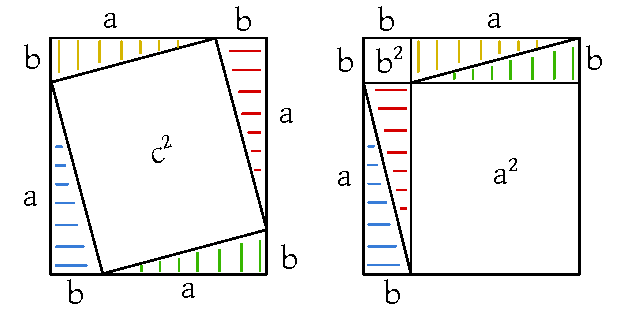
\includegraphics{img/03_pytha.pdf}
      \caption{Proof construction of the Pythagorem Theorem}
      \label{fig:pytha}
    \end{center}
  \end{figure}
\end{proof}

\dateref{2018/03/21}

The norm is given by
\[ \norm{\begin{pmatrix} a_1 \\ a_2 \\ a_3 \end{pmatrix}} = \sqrt{a_1^2 + a_2^2 + a_3^2} \]

\begin{definition}[Scalar product in $\mathbb R^2/\mathbb R^3$]
  \[ \angel{a, b} = \norm{a} \cdot \norm{b} \cdot \cos{\theta} \]
  where $\theta$ is the angle between vector $a$ and $b$.
\end{definition}

\begin{theorem}
  \[ \angel{a,a} = \norm{a}^2 \]
\end{theorem}

Recall that
\[ \cos{0} = 1 \qquad \cos{\frac\pi2} = 0 \qquad \cos{\pi} = -1 \qquad \cos{\frac32 \pi} = 0 \]
\[ \sin{0} = 0 \qquad \sin{\frac\pi2} = 1 \qquad \sin{\pi} = 0 \qquad \sin{\frac32 \pi} = -1 \]

\[ \sin\theta = \cos(\theta - \frac\pi2) \]
\[ \cos(\pi - \theta) = -\cos(\theta) \]
\[ \sin(-\theta) = \cos(\theta) \]
\[ \sin(\pi - \theta) = \sin(\theta) \]
\[ \sin(-\theta) = -\sin(\theta) \]

\begin{theorem} % Satz 8.2
  \begin{enumerate}
    \item $\angel{a,a} = \norm{a}^2$
    \item $\angel{a,a} = 0 \iff a = 0$
    \item $\angel{a,b} = 0 \iff a = 0 \lor b = 0 \lor \theta = \frac\pi2 \lor \theta = \frac32 \pi$, hence orthogonal
    \item $\angel{a,b} > 0 \iff$ acute angle
    \item $\angel{a,b} < 0 \iff$ obtuse angle
  \end{enumerate}
\end{theorem}

\begin{theorem} % Satz 8.3
  \label{satz83}
  \begin{enumerate}
    \item $\angel{a,b} = \angel{b,a}$
    \item $\angel{\lambda a, b} = \lambda \cdot \angel{a, b} = \angel{a, \lambda \cdot b}$
    \item $\angel{a+b, c} = \angel{a,c} + \angel{b, c}$
  \end{enumerate}
  Thus, linear in $a$ and $b$. Thus, bilinear.
\end{theorem}

\begin{proof}
  \begin{enumerate}
    \item[2.]
      Assume $\lambda > 0$. Angle stays the same.
      \[ \angel{\lambda a, b} = \norm{\lambda a} \cdot \norm{b} \cdot \cos\theta = \lambda \cdot \norm{a} \cdot \norm{b} \cdot \cos\theta \]
      Assume $\lambda < 0$. $\theta$ becomes $\pi - \theta$.
      \[ \angel{\lambda a, b} = \norm{\lambda a} \cdot \norm{b} \cdot \cos(\pi - \theta) = \card{\lambda} \cdot \norm{a} \cdot \norm{b} \cdot (-\cos(\theta)) = \lambda \cdot \norm a \cdot \norm b \]
    \item[3.]
      Let $\norm{c} = 1$. $\angel{a,c} = \norm a \cdot \cos\theta$.
      \[ \angel{a+b, c} = \angel{a,c} + \angel{b,c} \]
      Projections will add up.

      In the generic case:
      \begin{align*}
        \angel{a+b, c} &= \angel{a+b, \norm c \cdot \frac{c}{\norm{c}}} \\
          &\underbrace{=}_{\text{by (2.)}} \norm c \angel{a+b, \frac{c}{\norm{c}}} \\
%          &= \norm c \cdot \left(\angel{a, \frac{c}{\norm{c}} + \angel{b, \frac{c}{\norm{c}}\right) \\
%          &= \angel{a, c} + \angel{b, c}
      \end{align*}
  \end{enumerate}
\end{proof}

\begin{theorem} % Satz 8.4
  \[ \angel{\begin{pmatrix} a_1 \\ a_2 \\ a_3 \end{pmatrix}, \begin{pmatrix} b_1 \\ b_2 \\ b_3 \end{pmatrix}} = a_1 b_1 + a_2 b_2 + a_3 b_3 \]
\end{theorem}

\begin{proof}
  \begin{align*}
    \angel{a}{b} &= \angel{a_1 e_1 + a_2 e_2 + a_3 e_3, b} \\
      &= a_1 \angel{e_1, b} + a_2 \angel{e_2, b} + a_3 \angel{e_3, b} \\
      &= a_1 b_1 + a_2 b_2 + a_3 b_3 \\
    \angel{e_i,b} &= \angel{e_i, b_1 e_1 + b_2 e_2 + b_3 e_3} \\
      &= b_1 \angel{e_i, e_1} + b_2 \angel{e_i, e_2} + b_3 \angel{e_i, e_3} \\
      &= b_1 \delta_{i1} + b_2 \delta_{i2} + b_3 \cdot \delta_{i3} \\
      &= b_i
  \end{align*}
\end{proof}

In this chapter, we will talk about vector spaces in which we will discuss scalar products with properties 1--3 from Theorem~\ref{satz83}.
\[ \text{in } \mathbb R^n: \qquad \angel{x,y} = \sum_{i=1}^n x_i y_i \]
\[ \text{in } V \subseteq \mathbb R^\infty: \qquad \angel{x,y} = \sum_{i=1}^\infty x_i y_i \]
if convergent! For this space, $(e_i)_{i \in \mathbb N}$ is a basis.
\[ \text{in } C[a,b] \qquad \angel{f,g} = \int f(x) g(x) \, dx \]
is the Delta function.

Or better: $(\sin{nx})_{n \in \mathbb N} \cup (\cos{nx})_{n \in \mathbb N}$.

\[ \int_0^{2\pi} \sin(nx) \cos(mx) \, dx = 0 \forall m,n \]
\[ \int_0^{2\pi} \sin(nx) \sin(mx) \, dx = 0 \text{ if } m \neq n \]

1768/03/21 J. Fourier

\begin{theorem}[1822 Fourier]
  Every function $f$ in $[0,2\pi]$ can be denoted as
  \begin{align*}
    f(x) &= \sum_{n=0}^\infty a_n \cos(nx) + \sum_{n=1}^\infty b_n \sin(nx) \\
    a_n &= \angel{f, \cos(nx)} = \int_0^{2\pi} f(x) \cos(nx) \, dx \\
    b_n &= \angel{f, \sin(nx)} = \int_0^{2\pi} f(x) \sin(nx) \, dx
  \end{align*}
  This theorem cannot be proven, because it depends on the definition of \enquote{function}.
  The answer to the question, which functions satisfy this theorem, is an open research topic.
\end{theorem}

\subsection{Law of cosines}

\begin{theorem}[Law of cosines]
  In German, \foreignlanguage{german}{\enquote{Kosinussatz}}.

  \[ c^2 = a^2 + b^2 - 2ab \cos{\gamma} \]

  \begin{align*}
    \norm{\rh{c}}^2 &= \norm{\rh{b} - \rh{a}}^2 \\
      &= \angel{\rh{b} - \rh{a}, \rh{b} - \rh{a}} \\
      &= \angel{\rh{b}, \rh{b}} - \angel{\rh{a}, \rh{b}} - \angel{\rh{b} - \rh{a}} + \angel{\rh{a}, \rh{a}} \\
      &= \norm{b}^2 - 2 \norm{a} \norm{b} \cos\gamma + \norm{a}^2
  \end{align*}
\end{theorem}

\[ \norm a \cdot \norm b \cdot \sin\theta = \text{ area of the spanned parallelogram} \]

How to find an orthogonal vector?

\begin{remark}[Orthogonal vector in $\mathbb R^2$]
  Find $\vec{b}$ such that $\angel{\rh{a}, \rh{b}} = 0$, $a_1 b_1 + a_2 b_2 = 0$. For example, $b_1 = a_2$ and $b_2 = -a_1$.
  \[ \rh{a} = \begin{pmatrix} a_1 \\ a_2 \end{pmatrix} \qquad \rh{b} = \begin{pmatrix} a_2 \\ -a_1 \end{pmatrix} \]
\end{remark}

\subsection{Outer product}

\index{Outer product}
\index{Cross product}
\begin{definition} % 8.7
  Called \emph{outer product} (only in $\mathbb R^3$) or \emph{cross product}.

  Let $a,b \in \mathbb R^3$ and $a \times b$ is the vector which
  \begin{enumerate}
    \item $\norm{a \times b} = \norm{a} \cdot \norm{b} \cdot \sin{\theta}$ is the area of the spanned parallelogram.
    \item $a \times b \bot a \text{ and } b$
      \[ \angel{a \times b, a} = 0 \text{ and } \angel{a \times b, b} = 0 \]
    \item $(a, b, a \times b)$ is clockwise.
      \[ \text{When does } a \times b = 0 \text{ hold? } a = 0, b = 0, \sin\theta = 0, \text{ hence } \theta = 0 \lor \theta = \pi \]
      \[ \iff a,b \text{ are linear independent} \]
  \end{enumerate}
\end{definition}

\begin{theorem}
  \begin{itemize}
    \item $b \times a = -a \times b$
    \item $(\lambda a) \times b = \lambda (a \times b) = a \times (\lambda b)$
    \item $(a + b) \times c = a \times c + b \times c$
  \end{itemize}
\end{theorem}

\begin{proof}
  \begin{itemize}
    \item Orientation swaps.
    \item If $\lambda > 0$, it follows immediate.
      If $\lambda < 0$, lengths stay the same, but orientation swaps.
    \item If $c = 0$, it is trivial. If $c \neq 0$,
      \begin{figure}[!h]
        \begin{center}
          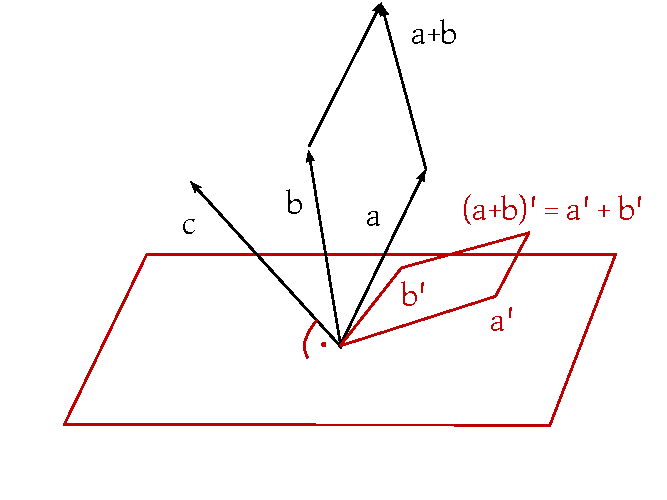
\includegraphics{img/04_apbmc_eq_amcpbmc.pdf}
        \end{center}
      \end{figure}
      E is the plane orthogonal to $c$. $a'$ and $b'$ are projections of $a$ and $b$ to $E$.

      \begin{enumerate}
        \item $(a+b)' = a' + b'$
        \item $a \times c = a' \times c$.
          \begin{align*}
            \norm{a \times c} &= \norm a \norm c \cdot \sin\theta \\
              &= \norm{a'} \cdot \norm{c} \\
              &= \norm{a' \times c}
          \end{align*}
          \begin{itemize}
            \item Orientation of $a \times c$ and $a' \times c$ is the same
            \item The plane, spanned by $c$ and $a$, is also spanned by $c$ and $a'$
          \end{itemize}

          \[ \norm{a'} = \norm{a} \cdot \underbrace{\cos(\frac\pi2}_{=\sin\theta} - \theta) \]
          Hence,
          \[ (a + b) \times c = (a + b)' \times c = (a' + b') \times c \stackrel!= a' \times c + b' \times c = a \times c + b \times c \]

          \[ (a' + b') \times c = a' + b' \]
          rotated by $90^\circ$ multiplied by $\norm{c}$
          \[ a' \times c = a' \]
          rotated by $90^\circ$ multiplied by $\norm{c}$

          \[ a' \times c + b' \times c = (a' + b') \times c \]

          The relation $u + v = w$ will be preserved under rotation by $90^\circ$ and multiplication with $\lambda$.
      \end{enumerate}
  \end{itemize}
\end{proof}

\begin{corollary} % 8.9
  The cross product is a map of $\mathbb R^3 \times \mathbb R^3 \to \mathbb R^3$
  such that
  \begin{itemize}
    \item bilinear
    \item antisymmetrical, $a \times b = -b \times a$
    \item $e_1 \times e_2 = e_3$, $e_2 \times e_3 = e_1$, $e_3 \times e_1 = e_2$
      \[ e_i \times e_j = e_k \cdot \sign{\pi} \qquad \pi = \begin{pmatrix} 1 & 2 & 3 \\ i & j & k \end{pmatrix} \]
  \end{itemize}
\end{corollary}

\begin{corollary}
  \[
    \begin{pmatrix} a_1 \\ a_2 \\ a_3 \end{pmatrix}
    \times \begin{pmatrix} b_1 \\ b_2 \\ b_3 \end{pmatrix}
    = \begin{bmatrix} a_2 b_3 - a_3 b_2 \\ a_3 b_1 - a_1 b_3 \\ a_1 b_2 - a_2 b_1 \end{bmatrix}
    = \begin{bmatrix}
      \begin{vmatrix} a_2 & b_2 \\ a_3 & b_3 \end{vmatrix} \\
      -\begin{vmatrix} a_1 & b_1 \\ a_3 & b_3 \end{vmatrix} \\
      \begin{vmatrix} a_1 & b_1 \\ a_2 & b_2 \end{vmatrix}
    \end{bmatrix}
    \underbrace{=}_{\text{by Laplace expansion along the third column\footnote{not an actual equality}}}
    \begin{vmatrix}
      a_1 & b_1 & e_1 \\
      a_2 & b_2 & e_2 \\
      a_3 & b_3 & e_3
    \end{vmatrix}
  \]
  % TODO footnote is invisible
\end{corollary}

\begin{proof}
  \begin{align*}
      &(a_1 e_1 + a_2 e_2 + a_3 e_3) \times (b_1 e_1 + b_2 e_2 + b_3 e_3) \\
      &= a_1 b_1 e_1 \times e_1 + a_1 b_2 e_1 \times e_2 + a_1 b_3 e_1 \times e_3 \\
      &+ a_2 b_1 e_2 \times e_1 + a_2 b_2 e_2 \times e_2 + a_2 b_3 e_2 \times e_3 \\
      &= a_3 b_1 e_3 \times e_1 + a_3 b_2 e_3 \times e_2 + a_3 b_3 e_3 \times e_3 \\
      &= a_1 b_2 e_3 - a_1 b_3 e_2 - a_2 b_1 e_3 + a_2 b_3 e_1 + a_3 b_1 e_2 - a_3 b_2 e_1 \\
      &= (a_2 b_3 - a_3 b_2) e_1 + (a_3 b_1 - a_1 b_3) e_2 + (a_1 b_2 - a_2 b_1) e_3
  \end{align*}
\end{proof}

\begin{theorem} % Satz 8.11
  \[ \angel{a \times b, c} = \begin{vmatrix} a_1 & b_1 & c_1 \\ a_2 & b_2 & c_2 \\ a_3 & b_3 & c_3 \end{vmatrix} \]
  This corresponds to the volume of the spanned parallelepiped (dt. \foreignlanguage{german}{\enquote{Spat}}).
  $\norm{a \times b}$ is the area of the parallelogram and $\norm{c}$ its height.

  Equivalently, $\begin{vmatrix} a_1 & a_2 \\ b_1 & b_2 \end{vmatrix}$ is the area of the parallelogram.
\end{theorem}

\begin{example} % Anwendung 8.12
  Let planes in $\mathbb R^3$ be given.
  \[ E = \setdef{x_0 + \lambda a + \mu b}{\lambda, \mu \in \mathbb R} \]
  \[ c = a \times b = \setdef{x \in \mathbb R^3}{x - x_0 \bot c} = \setdef{x \in \mathbb R^3}{\angel{x - x_0, c} = 0} \]
  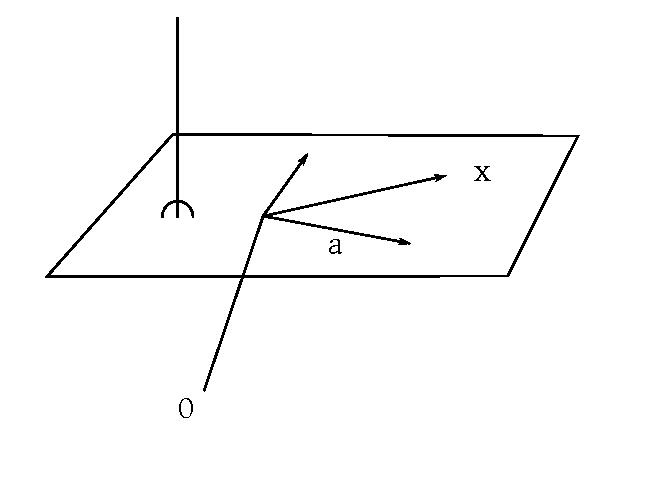
\includegraphics{img/05_application.pdf} % TODO
\end{example}

\subsection{Inner products and positive definiteness}
From now on $\mathbb K$ will be $\mathbb R$ or $\mathbb C$.

\begin{definition} % Definition 8.13
  An inner product on a vector space $V$ is a map
  \[ V \times V \to \mathbb K \]
  \[ (x,y) \mapsto \angel{x,y} \]
  \begin{enumerate}
    \item $\angel{x+y, z} = \angel{x,z} + \angel{y,z} \forall x,y,z \in V$
    \item $\angel{\lambda x, y} = \lambda \angel{x,y} \forall \lambda \in \mathbb K \forall x,y \in V$
    \item $\angel{y,x} = \overline{\angel{x,y}} \forall x,y \in V$
  \end{enumerate}
  where $\overline{\angel{x,y}}$ denotes the complex conjugate.

  \[
    \angel{x, \lambda y} \underbrace{=}_{\text{by (3)}} \overline{\angel{\lambda y, x}}
      \underbrace{=}_{\text{by (2)}} \overline{\lambda \angel{y, x}}
      = \overline{\lambda} \angel{x,y}
  \]

  Linear in $x$, semi-linear in $y$. Sesquilinear\footnote{In Latin, sesqui means $1.5$}.

  In physics, the notation is different:
  \[ \angel{x|y} \qquad \angel{\lambda x|y} = \overline{\lambda} \angel{x|y} \qquad \angel{x|\lambda y} = \lambda \angel{x|y} \]
  \[ |y\rangle \dots \text{ ket} \qquad \langle x| \dots \text{ bra} \]
  \[ \angel{x|y} \qquad \text{ bracket} \]

  The inner product is called positive-semidefinite, if
  \[ \angel{x,x} \geq 0 \forall x \in X \]
  if additionally $\angel{x,x} = 0 \iff x = 0$, then $\angel{,}$ is called positive definite.
\end{definition}

\dateref{2018/04/09. Easter holidays finished.}

\begin{lemma} % 8.14
  \begin{enumerate}
    \item $\angel{x, y + z} = \angel{x, y} + \angel{x, z}$
    \item $\angel{x, \lambda y} = \overline{\lambda} \cdot \angel{x, y}$
    \item $\angel{x, 0} = 0$
  \end{enumerate}
\end{lemma}

\index{Positive semidefinite inner product}
\index{Positive inner product}
\index{Negative definite inner product}
\index{Indefinite inner product}
\index{Hermitian form}
\index{Unitary product}
\begin{definition}
  An inner product is \emph{positive semidefinite}, if $\angel{x, x} \geq 0$.
  Is \emph{positive definite}, if $\angel{x, x} > 0$ for all $x \neq 0$.
  Is \emph{negative definite}, if $\angel{x, x} < 0$ for all $x \neq 0$.
  Is \emph{indefinite}, if neither positive nor negative semidefinite.

  A positive definite product is called \emph{scalar product}.
  A positive definite product is in \emph{Hermitian form}, if $\mathbb K = \mathbb C$.
  A positive definite product is also called \emph{unitary product}, if $\mathbb K = \mathbb C$.

  So quadratic form over $\mathbb R$ and Hermitian form over $\mathbb C$.
\end{definition}

\begin{example} % 8.15
  \begin{itemize}
    \item 
      Let $V = \mathbb R^n$.
      \[
        \angel{\begin{pmatrix} x_1 \\ \vdots \\ x_n \end{pmatrix}, \begin{pmatrix} y_1 \\ \vdots \\ y_n \end{pmatrix}}
        = \sum_{i=1}^n x_i y_i
      \]
      Let $V = \mathbb C^n$.
      \[
        \angel{\begin{pmatrix} x_1 \\ \vdots \\ x_n \end{pmatrix}, \begin{pmatrix} y_1 \\ \vdots \\ y_n \end{pmatrix}}
        = \sum_{i=1}^n x_i \overline{y_i}
        \implies \angel{x, x} = \sum_{i=1}^n x_i \overline{x_i} = \sum_{i=1}^n \card{x_i}^2 \geq 0
      \]
      $\to$ positive definite.

    \item
      Another example: let $A \in \mathbb R^{n \times n}$.
      Let $x, y \in \mathbb R^n$.
      \begin{align*}
        \angel{x, y}_A &= x^t \cdot A \cdot y \qquad \text{ is bilinear} \\
          &= \sum_{i=1}^n x_i \sum_{j=1}^n a_{ij} y_j = \sum_{i,j=1}^n a_{ij} x_i y_j
      \end{align*}
      hence $\angel{x, y}_A = \angel{y, x}_A$.
      It must hold that
      \[ \sum_{i,j=1}^n a_{ij} x_i y_j = \sum_{i,j=1}^n a_{ij} y_i x_j \forall x,y \]
      We let $x = e_k$ and $y = e_l$.
      \[ \implies a_{kl} = a_{lk} \forall k,l \]
      Hence $A = A^T$. $A$ is symmetrical.

      Let $A \in \mathbb C^{n \times n}$. Let $x, y \in \mathbb C^n$.
      \[ \angel{x, y}_A = \sum_{i=1}^n \sum_{j=1}^n x_i a-{ij} \overline{y_j} \]
      \[ \angel{x,y}_A = \angel{y,x}_A \forall x,y \]
      \[ \iff A^T = \overline{A} \qquad \text{ is in Hermitian form} \]
      \[ a_{ji} = \overline{a_{ij}} \forall i ,j \]

    \item
      \[ V = C[a,b] = \set{f: [a,b] \to \mathbb K \text{ continuous}} \]
      \[ \angel{f,g} = \int_a^b f(t) \overline{g(t)} \, dt \qquad \text{ is a scalar product} \]
      \[ \angel{f,f} = \int_a^b \card{f(t)}^2 \, dt \geq 0 \]

    \item
      Consider $V = l_2$ ($\mathbb R^{\infty}$ would be too large) where $l_2 = \setdef{(x_n)_{n\in\mathbb N}}{x_n \in \mathbb R, \sum_{n=1}^\infty x_n^2 < \infty}$.
      \[ \angel{x, y} = \sum_{n=1}^\infty x_n y_n \qquad \text{ is a scalar product} \]
      Does it converge? This is not obvious.

      Fourier claimed that this example (4) and example (3) are the same.
      He claimed every function can be written as $f(x) = \sum_{n=0}^\infty a_n e^{inx}$.

      \[ x \cdot x = \angel{x, x} = \sum_{i=1}^n x_i^2 = \norm{x}^2 \]
  \end{itemize}
\end{example}

\index{Norm}
\begin{definition}
  Let $V$ be a vector space.
  A \emph{norm} on $V$ is a map $\norm{\cdot}: V \to [0,\infty[$
  such that
  \begin{enumerate}
    \item $\norm{x} \geq 0$ and $\norm{x} = 0 \iff x = 0$
    \item $\norm{\lambda \cdot x} = \card{\lambda} \cdot \norm{x} \qquad \forall \lambda \in K, \forall x \in V$
    \item $\norm{x + y} \leq \norm{x} + \norm{y}$ is the triangle inequality
  \end{enumerate}
\end{definition}

\begin{remark}
  Every norm is a metric with $d(x,y) = \norm{x - y}$.

  $d$ is translation invariant. $d(x + x_0, y + x_0) = d(x, y)$.
  This is compatible to a vector space.

  In a black hole ($\to$ physics), you have a different metric in every point (Riemannian geometry): $\angel{x,y}_{A(x,y)}$.
\end{remark}

\index{Euclidean norm}
\begin{example}
  Let $V = \mathbb R^n$.
  \begin{itemize}
    \item $\norm{x}_2 = \left(\sum_{i=1}^n x_i^2\right)$ is called \emph{euclidean norm}.
    \item $\norm{x}_1 = \sum_{i=1}^n \card{x_i}$ is called \emph{$l^1$ norm} or \emph{Manhattan norm}.
    \item $\norm{x}_{\infty} = \max\setdef{\card{x_i}}{i = 1, \dots, n}$
  \end{itemize}
  Let $V = C[a,b]$.
  \begin{itemize}
    \item \[ \norm{f}_1 = \int_a^b \card{f(t)} \, dt \]
      $L^1$-norm, gives rise to the Lebesgue integral.
    \item \[ \norm{f}_\infty =\ max_{t \in [\overline{a}, b]} \card{f(t)} \qquad \text{ is a $L^\infty$-norm} \]
    \item \[ \norm{f}_2 = \left(\int \card{f(t)}^2 \, dt \right)^{\frac12} \]
  \end{itemize}
\end{example}

\begin{theorem} % 8.19
  \label{thm:t819}
  Let $\angel{,}$ be a scalar product in $V$ (hence, positive-definite inner product).
  Then $\norm{x} = \sqrt{\angel{x,x}}$ is a norm on $V$.
\end{theorem}

\begin{proof}
  \begin{itemize}
    \item $\norm{x} \geq 0, \norm{x} = 0 \iff \angel{x,x} = 0 \iff x = 0$
    \item $\norm{\lambda x} = \sqrt{\angel{\lambda x, \lambda x}} = \sqrt{\lambda \cdot \overline{\lambda} \cdot \angel{x,x}} = \sqrt{\lambda^2 \cdot \angel{x,x}} = \card{\lambda} \cdot \sqrt{\angel{x,x}}$
    \item Triangle inequality
  \end{itemize}
\end{proof}

\subsection{Cauchy-Bunyakovskii-Schwarz inequality}

\begin{lemma}[Cauchy-Bunyakovskii-Schwarz inequality] % 8.20
  \label{thm:cbs}
  Cauchy (1789--1857) for $\mathbb R^n$,
  Bunyakovskii (1804--1889) for $C[a,b]$,
  Schwarz (1843--1921) generically.

  \[ \card{\angel{x,y}} \leq \norm{x} \cdot \norm{y} \]

  Hence, $l^2$ if $\sum_{n=1}^\infty x_n^2 < \infty$ and $\sum_{n=1}^\infty y_n^2 < \infty$.
  $\angel{x,x} < \infty$ and $\angel{y,y} < \infty$.
  \[ \implies \sum x_n y_n \leq \sqrt{\sum x_n^2} \sqrt{\sum y_n^2} \]

  If $\card{\angel{x,y}} = \norm{x} \cdot \norm{y} \iff x,y \text{ are linear dependent}$.
\end{lemma}

\begin{proof}
  Now we can continue with part 3 of the proof of Theorem~\ref{thm:t819}.
  Triangle inequality:
  \begin{align*}
    \norm{x + y}^2 &= \angel{x + y, x + y} \\
      &= \angel{x,x} + \angel{x,y} + \angel{y,x} + \angel{y,y} \\
      &\leq \norm{x}^2 + 2 \card{\angel{x, y}} + \norm{y}^2 \\
      &\leq \norm{x}^2 + 2 \norm{x} \norm{y} + \norm{y}^2 \\
      &= \left(\norm x + \norm y\right)^2
  \end{align*}
\end{proof}

\begin{proof}[Proof of CBS inequality, Lemma~\ref{thm:cbs}]
  \begin{description}
    \item[Case 1: $y = 0$] trivial
    \item[Case 2: $y \neq 0$]
      Let $\lambda \in \mathbb K$ be arbitrary.
      \begin{align*}
        0 &\leq \angel{x - \lambda y, x - \lambda y} \\
          &= \angel{x, x} - \angel{x, \lambda y} - \angel{\lambda y, x} + \angel{\lambda y, \lambda y} \\
          &= \angel{x, x} - \overline{\lambda} \angel{x,y} - \lambda \angel{y,x} + \card{\lambda}^2 \angel{y,y} \\
        \intertext{
          This holds for all $\lambda$, hence also for $\lambda = \frac{\angel{x,y}}{\angel{y,y}}$.
          Because $y \neq 0 \implies \angel{y,y} > 0$, we can divide.
        }
          &= \angel{x,x} - \frac{\overline{\angel{x,y}}}{\angel{y,y}} \cdot \angel{x,y} - \frac{\angel{x,y}}{\angel{y,y}} \cdot \angel{y,x} + \frac{\card{\angel{x,y}}^2}{\angel{y,y}^2} \cdot \angel{y,y} \\
          &= \angel{x,x} - \frac{\card{\angel{x,y}}^2}{\angel{y,y}} - \frac{\card{\angel{x,y}}^2}{\angel{y,y}} + \frac{\card{\angel{x,y}}^2}{\angel{y,y}} \\
          &= \norm{x}^2 - \frac{\card{\angel{x,y}}^2}{\norm{y}^2} \\
          &\implies \norm{x}^2 \cdot \norm{y}^2 - \card{\angel{x,y}}^2 \geq 0
      \end{align*}
  \end{description}
\end{proof}

\begin{proof}[Alternative proof of CBS inequality in $\mathbb R^n$]
  \begin{align*}
    0 &\leq \sum_{i=1}^n \sum_{j=1}^n (x_i y_j - x_j y_i)^2 \\
      &= \sum_{i,j=1}^n \left(x_i^2 y_j^2 - 2 x_i y_j x_j y_i + x_j^2 y_i^2\right) \\
      &= \sum_{i,j}^n x_i^2 y_j^2 - 2 \sum_{i,j} x_i x_j y_i y_j + \sum_{i,j} x_j^2 y_i^2 \\
      &= 2 \sum_i x_i^2 \sum_j y_j^2 - 2 \sum_i x_i y_i \sum_j x_j y_j \\
      &= 2 \norm{x}^2 \norm{y}^2 - 2 \angel{x,y}^2 \\
      &\leadsto \norm{x}^2 \norm{y}^2 = \angel{x,y}^2 + \frac12 \sum_i \sum_j (x_i y_j - x_j y_i)^2
  \end{align*}
  So for $n=3$, $\norm{x}^2 \norm{y}^2 = \angel{x,y}^2 + \norm{x \times y}^2$.
  Hence, equality is given iff $x$ and $y$ are linear dependent.

  In the general case:
  If $\card{\angel{x,y}} = \norm{x} \cdot \norm{y}$.
  From the proof, it follows that
  $\exists \lambda: \angel{x - \lambda y, x - \lambda y} = 0$
  \[ \implies x - \lambda y = 0 \implies x,y \text{ are linear independent} \]
\end{proof}

\begin{theorem} % 8.21
  Let $V$ be a vector space over $\mathbb K = \mathbb R$ or $\mathbb C$.
  Let $B = \set{b_1, \dots, b_n}$ is a basis.
  $\angel{,}$ is an inner product.
  What does $\angel{,}$ look like in regards of the coordinate?

  There exists a unique matrix $A$ in Hermitian form (hence, $a_{ij} = \overline{a_{ji}}, A = \overline{A^T}$)
  such that $\forall x,y \in V: \angel{x,y} = \Phi_B(x)^T \cdot A \cdot \overline{\Phi_B(y)}$.
  If $\angel{,}$ is positive definite, $A$ is regular.
\end{theorem}

\begin{remark}
  \[ \angel{x,y} = \sum x_i \overline{y_i} \]
  corresponds to $A = I$.
  \[ x^T \cdot I \cdot \overline{y} = x^T \cdot \overline{y} \]

  How about $A = -I$.
  \[ \angel{x,y}_A = -\sum x_i \overline{y}_i \]
  This is not a scalar product (because of negative definiteness).
\end{remark}

\begin{proof}
  Let $x = \sum_{i=1}^n \xi_i b_i, y = \sum_{j=1}^n \eta_j b_{j}$.
  \begin{align*}
    \angel{x,y} &= \angel{\sum_{i=1}^n \xi_i b_i, \sum_{j=1}^n \eta_j b_j} \\
      &= \sum_{i=1}^n \xi_i \sum_{j=1}^n \overline{\eta_j} \underbrace{\angel{b_i, b_j}}_{\eqqcolon a_{ij} \text{ is unique } a_{ij} = \angel{b_i, b_j}} \\
      &= \sum_{i=1}^n \sum_{j=1}^n \xi_i a_{ij} \overline{\eta}_j \\
      &= \xi^T \cdot A \cdot \overline{\eta} \\
      &= \Phi_B(x)^T \cdot A \cdot \Phi_B(y) \\
    a_{ji} &= \angel{b_j, b_i} = \overline{\angel{b_i, b_j}} = \overline{a_{ij}}
  \end{align*}

  Show: If $\angel{,}$ is positive definite, then $A$ is regular.
  It suffices to show that $\operatorname{ker}{A} = \set{0}$.

  Assume: $A \cdot \xi = 0 \implies \xi^T \cdot A \cdot \xi = 0$.
  Let $x = \sum_{i=1}^n \xi_i b_i \implies \angel{x,x} = 0 \implies x = 0 \implies \xi = \Phi_B(x) = 0$
\end{proof}

\index{Conjugate transpose}
\index{Self-adjoint matrix}
\index{Hermitian matrix}
\begin{definition} % 8.22
  Let $A \in \mathbb C^{n \times n}$.
  The matrix $A^* \coloneqq \overline{A^T}$ ($(A^*)_{ij} = \overline{a_{ji}}$)
  is called \emph{conjugate transpose}.

  $A$ is called \emph{self-adjoint} if $A = A^*$.
  $A$ is called \emph{symmetrical} if $A = \overline{A}$ and $\mathbb K = \mathbb R$
  or $A$ is called \emph{Hermitian} if $A = A^*$ and $\mathbb K = \mathbb C$.

  $A = A^*$ is called (positive/negative) (semidefinite/definite) if the corresponding sesquilinear form
  \[ \angel{\xi, \eta}_A = \xi^T \cdot A \cdot \overline{\eta} \]
  Hence, $\xi^T A \overline{\xi} \geq 0 \forall \xi \neq 0$ is positive definite, has the corresponding property or
  $\xi^T A \overline{\xi} > 0 \forall \xi \neq$ is positive semidefinite, has the corresponding property.

  $\xi^T A \overline{\xi} \leq 0 \forall \xi \neq$ is negative definite or
  $\xi^T A \overline{\xi} < 0 \forall \xi \neq$ is negative semidefinite.

  If $\exists \xi: \xi^T A \overline{\xi} > 0$ and $\exists \eta: \eta^T A \overline{\eta} < 0$, then $A$ is called indefinite.
\end{definition}

\dateref{2018/04/11}

Inner product: $\angel{x,y}$
\begin{itemize}
  \item $\forall x: \angel{x,x} \geq 0$ positive semi-definite
  \item $\forall x \neq 0: \angel{x,x} > 0$ positive definite
\end{itemize}
in regards of basis $b_1, \dots, b_n$.

\[ \angel{x,y} = \sum a_{ij} \xi_i \overline{\eta_j} \]
\[ a_{ij} = \angel{b_i, b_j} \]

\begin{remark}
  $A = A^*$ is called \emph{positive semidefinite} if $A \geq 0$ if $\forall \xi: \xi^T A \overline{\xi} \geq 0$.

  $A = A^*$ is called \emph{positive definite} if $A > 0$ if $\forall \xi \in \mathbb K^n\setminus \set{0}: \xi^T A \overline{\xi} > 0$
  with $\xi^T A \overline{\xi} = \sum_{i=1} \sum_{j=1} TODO$.
\end{remark}

\begin{example}
  \[ A = I > 0 \]
  \[ \xi^T I \overline{\xi} = \sum_{i=1}^n \xi_i \overline{\xi_i} = \sum \card{\xi_i}^2 > 0 \qquad \text{ if } \xi \neq 0 \]
  \[ A = -I < 0 \text{ is negative definite} \]
  \[
    A = \begin{bmatrix}
      1 &        &   &    &        & \\
        & \ddots &   &    &        & \\
        &        & 1 &    &        & \\
        &        &   & -1 &        & \\
        &        &   &    & \ddots & \\
        &        &   &    &        & -1
    \end{bmatrix}
  \]
  is indefinite:
  \[ e_1^T A e_1 > 0 \qquad e_n^T A e_n < 0 \]
\end{example}

\begin{remark}
  For a diagonal matrix
  \[ A = \begin{bmatrix} a_1 &  & 0 \\ & \ddots & \\ 0 &  & a_n \end{bmatrix} \]
  $A = A^* \iff a_i = \overline{a}_i$, hence for all $a_i \in \mathbb R$.

  For a diagonal matrix it holds that
  \begin{align*}
    A > 0 & \text{ if all } a_i > 0: \xi^T A \overline{\xi} = \sum_{i=1}^n a_i \card{\xi_i}^2 \geq 0 \\
    A \leq 0 & \text{ if all } a_i \geq 0 \text{ if } \xi^T A \overline{\xi} = 0 \implies \text{ all } a_i \cdot \card{\xi_i}^2 = 0 \\
    A < 0 & \text{ if all } a_i < 0 \\
    A \leq 0 & \text{ if all } a_i \leq 0 \\
    \text{indefinite} & \text{ if } \exists i: a_i > 0 \exists j: a_j < 0
  \end{align*}
\end{remark}

\begin{remark}
  Remember, that the rank of matrix satisfies:
  \[ \exists P,Q \in \operatorname{GL}(n): PAQ = \begin{pmatrix} 1 & & & \\ & 1 & & \\ & & \ddots & \\ & & & 0 \end{pmatrix} \]
  \[ A \sim PAQ \text{ is equivalent} \]
\end{remark}

\subsection{Congruence of matrices}

\index{Congruence of matrices}
\begin{definition}[Congruence] % Definition 8.23
  Consider two self-adjoint matrices $A, B \in \mathbb K^{n \times n}$ are called congruent (denoted $A \hat= B$)
  if $\exists C \in \operatorname{GL}(n, \mathbb K)$ such that $C^* AC = B$.
\end{definition}

\begin{remark}
  $C$ is invertible, hence $C^T$ is invertible.
  \[ (C^T)^{-1} = (C^{-1})^T \qquad (C^{-1})^T \cdot C^T = (C \cdot C^{-1})^T = I^T = I \]
  \[ (\overline{A}^{-1}) = \overline{A^{-1}} \]
  \[ (AB)^* = \overline{(AB)^T} = \overline{B^T A^T} = \overline{B^T} \overline{A^T} = B^* \cdot A^* \]

  $C^* AC$ is self-adjoint.
  \[ (C^* AC)^* = C^* \cdot A^* \cdot (C^*)^* = C^* \cdot A \cdot C \]
\end{remark}

\begin{theorem} % Satz 8.24
  Every Hermitian matrix is congruent to a diagonal matrix of structure:
  \[
    \begin{bmatrix}
      1 &   &        &    &    &        &    &   &        & \\
        & 1 &        &    &    &        &    &   &        & \\
        &   & \ddots &    &    &        &    &   &        & \\
        &   &        & 1  &    &        &    &   &        & \\
        &   &        &    & -1 &        &    &   &        & \\
        &   &        &    &    & \ddots &    &   &        & \\
        &   &        &    &    &        & -1 &   &        & \\
        &   &        &    &    &        &    & 0 &        & \\
        &   &        &    &    &        &    &   & \ddots & \\
        &   &        &    &    &        &    &   &        & 0
    \end{bmatrix}
  \]
\end{theorem}

\begin{proof}
  The proof is given by an algorithm.

  We construct matrix C inductively such that
  \[ C^* A C = \operatorname{diag}(\pm 1, \dots, 0) \]
  Consider $n = 1$.
  \[ A = [a_{11}] \]
  If $a_{11} = 0$ where $a_{11} \in \mathbb R$, we don't have to do anything.
  If $a_{11} \neq 0$,
  \[ C = \left[\frac{1}{\sqrt{\card{a_{11}}}}\right] \]
  \[ C^* AC = \left[\frac{1}{\sqrt{\card{a_{11}}}} \cdot a_{11} \cdot \frac{1}{\sqrt{\card{a_{11}}}}\right] = \left[\operatorname{sign}(a_{11})\right] \]

  \begin{example} % 8.25
    \label{ex825}
    \[
      A = \begin{bmatrix}
        0 & 1 & i \\
        1 & 0 & 1 \\
        -i & 1 & 0
      \end{bmatrix}
    \]
  \end{example}

  Then $n-1 \to n$:
  \begin{description}
    \item[Case 1: $A = 0$] nothing to do.
    \item[Case 2: $a_{11} = 0$]
      \begin{description}
        \item[Case 2a:] 
          \[
            \exists j: a_{jj} \neq 0:
            \begin{bmatrix}
              0 & & & & \\
                & & a_{jj} & & \\
            \end{bmatrix}
          \]
          \[
            T_{(1,j)} = \begin{bmatrix}
              0 &   & & & & & & 1 \\
                & 1 & & & & & & \\
                &   & \ddots & & & & & \\
                &   &    & 1 & & & & \\
                &   &    & & 0 & & & \\
                &   &    & &   & 1 & & \\
                &   &    & &   &  & \ddots & \\
              1 &   &    & &   &  &  & 1 \\
            \end{bmatrix}
            = T^*_{(ij)}
          \]
          Permutation matrix that swaps 1 with $j$.

          \[
            T_{(1j)}^* A T_{(1j)} =
            \begin{bmatrix}
              a_{ji}  & \ldots & \ldots \\
              \vdots  & \ddots &   \\
              \vdots  &        & 0 \\
            \end{bmatrix}
          \]
          where $T_{(1j)}^*$ exchanges $j$-th and first row
          and $T_{(1j)}$ exchanges $j$-th and first column.
        \item[Case 2b]:
          all $a_{jj} = 0$. Choose $i,j$ such that $a_{ij} \neq 0$.
          \[ C = I + E_{ij} e^{i\theta} \]
          where $\theta$ such that $a_{ij} = e^{i\theta} \card{a_{ij}}$.

          \begin{example}
            $a_{12} \neq 0$
            \[
              C_1 = \begin{bmatrix}
                1 & 1 & \\
                  & 1 & \\
                  &   & 1
              \end{bmatrix}
            \] \[
              C_1^* A C_1 = \begin{bmatrix}
                1 & 0 & 0 \\
                1 & 1 & 0 \\
                0 & 0 & 1
              \end{bmatrix} \cdot \begin{bmatrix} 
                0 & 1 & i \\
                1 & 0 & 1 \\
                -i & 1 & 0
              \end{bmatrix} \cdot \begin{bmatrix}
                1 & 1 & 0 \\
                0 & 1 & 0 \\
                0 & 0 & 1
              \end{bmatrix}
            \] \[
              \begin{bmatrix}
                0 & 1 & i \\
                1 & 1 & 1+i \\
                -i & 1 & 0
              \end{bmatrix} \cdot \begin{bmatrix}
                0 & 1 & i \\
                1 & 2 & 1+i \\
                -i & 1-i & 0
              \end{bmatrix}
            \]
          \end{example}

          In the general case:
          \[ C^* AC = (I + E_{ji} e^{-i\theta}) A (I + E_{ij} e^{i\theta}) \]
          \begin{align*}
            (C^* AC)_{jj} &= \left(A + E_{ji} e^{-i\theta} A + AE_{ij} e^{+i\theta} + E_{ji} A E_{ij}\right)_{jj} \\
              &=
                \underbrace{a_{jj}}_{=0} +
                \underbrace{(E_{ji} e^{-i\theta} A)_{jj}}_{e^-i\theta a_{jj} = \card{a_{ij}}} +
                \underbrace{(AE_{ij} e^{+i\theta})_{jj}}_{a_{ji} e^{+i\theta} = \overline{a_{ij}} e^{i\theta} = \card{a_{ij}}} +
                \underbrace{a_{ii}}_{=0} \\
              &= 2 \card{a_{ij}}
          \end{align*}
          Case 2a is shown.

          \begin{example}
            \[
              C_2 = \begin{bmatrix}
                0 & 1 & \\
                1 & 0 & \\
                  &   & 1
              \end{bmatrix} = T_{(12)}
            \]
          \end{example}

          \[
            A_2 = C_2^* A_1 C_2 = \begin{bmatrix}
              0 & 1 & 0 \\
              1 & 0 & 0 \\
              0 & 0 & 1
            \end{bmatrix} \cdot \begin{bmatrix}
              0 & 1 & i \\
              1 & 2 & i+1 \\
              -i & 1-i & 0
            \end{bmatrix} \cdot \begin{bmatrix}
              0 & 1 & 0 \\
              1 & 0 & 0 \\
              0 & 0 & 1
            \end{bmatrix}
          \] \[
            \begin{bmatrix}
              1 & 2 & i+1 \\
              0 & 1 & i \\
              -i & 1-i & 0
            \end{bmatrix} \cdot \begin{bmatrix}
              2 & 1 & 1+i \\
              1 & 0 & i \\
              1-i & -i & 0
            \end{bmatrix}
          \]
      \end{description}
    \item[Case 3]
      $a_{11} \neq 0$
      \[
        C = \begin{bmatrix}
          1 & -\frac{a_{12}}{a_{11}} & -\frac{a_{13}}{a_{11}} & \dots  & -\frac{a_{in}}{a_{11}} \\
            & 1                      &                 \ldots &     0  &         0 \\
            & \vdots                 & 1                      &        &         0 \\
            & 0                      &                        & \ddots &           \\
            & 0                      & 0                      & \ldots &         1 \\
        \end{bmatrix}
      \]

      \begin{example}
        \[
          C_3 = \begin{bmatrix}
            1 & -\frac12 & -\frac{1+i}2 \\
              & 1        & \\
              &          & 1
          \end{bmatrix}
        \] \[
          A_3 = C_3^* A_2 C_3 = \begin{bmatrix}
            1 & 0 & 0 \\
            -\frac12 & 1 & 0 \\
            -\frac{1-i}{2} & 0 & 1
          \end{bmatrix} \cdot \begin{bmatrix}
            2 & 1 & 1+i \\
            1 & 0 & i \\
            1-i & -i & 0
          \end{bmatrix} \cdot \begin{bmatrix}
            1 & -\frac12 & -\frac{1+i}{2} \\
            0 & 1 & 0 \\
            0 & 0 & 1
          \end{bmatrix}
        \] \[
          \begin{bmatrix}
            2 & 1 & 1+i \\
            0 & -\frac12 & \frac12 (-i + i) \\
            0 & \frac12 (-1-i) & -1
          \end{bmatrix} \cdot \begin{bmatrix}
            2 & 0 & 0 \\
            0 & -\frac12 * \frac{-1+i}{2} \\
            0 & \frac{-1-i}{2} & -1
          \end{bmatrix}
        \]
      \end{example}
      \[
        C^* AC = \begin{bmatrix}
          a_{11} & 0 & \ldots & 0 \\
          0      &   &        &   \\
          \vdots &   &        &   \\
          0      &   &        & \tilde{A}
        \end{bmatrix}
      \] \[
        \tilde{A} \in \mathbb K^{(n-1) \times (n-1)}
      \] \[
        \tilde{A} = \tilde{A}^*
      \]

      \[
        C' = \begin{bmatrix}
          \frac{1}{\sqrt{\card{a_{11}}}} &  & & 0 \\
             & 1 & & \\
             &   & \ddots & \\
          0  &   &        & 1
        \end{bmatrix}
      \] \[
        (C')^* (C^* AC) C' = \begin{bmatrix}
          \frac{a_{11}}{\card{a_{11}}} & 0 &  & 0 \\
          0 & & & \\
          \vdots & & & \\
          0 & & & \tilde{A} \\
        \end{bmatrix}
        \text{ where } \frac{a_{11}}{\card{a_{11}}} = \pm 1
      \]
      Apply this algorithm to $\tilde{A}$.

      \begin{example}[Part 4]
        \[ C_4 = \begin{bmatrix} \frac1{\sqrt2} & & \\ & 1 & \\ & & 1 \end{bmatrix} \]
        \[ A_4 = C_4^* A_3 C_4 = \begin{bmatrix}
          1 & 0 & 0 \\
          0 & -\frac12 & \frac{-1+i}{2} \\
          0 & \frac{-1-i}{2} & -1
          \end{bmatrix}
        \] \[
          \tilde A = \begin{bmatrix}
            -\frac12 & \frac{-1+i}{2} \\
            \frac{-1-i}{2} & -1
          \end{bmatrix}
        \] \[
          C_5 = \begin{bmatrix}
            1 & & \\
              & 1 & -1+i \\
              & 0 & 1
          \end{bmatrix}
        \] \[
          A_5 = C_5^* A_4 C_5 = \begin{bmatrix}
            1 & 0 & 0 \\
            0 & 1 & 0 \\
            0 & -1-i & 1
          \end{bmatrix} \cdot \begin{bmatrix}
            1 & 0 & 0 \\
            0 & -\frac12 & \frac{-1+i}{2} \\
            0 & \frac{-1-i}{2} & -1
          \end{bmatrix} \cdot \begin{bmatrix}
            1 & 0 & 0 \\
            0 & 1 & -1+i \\
            0 & 0 & 1
          \end{bmatrix}
        \] \[
          A_5 = \begin{bmatrix}
            1 & 0 & 0\\
            0 & -\frac12 & \frac{-1+i}{2} \\
            0 & 0 & 0
          \end{bmatrix} \cdot \begin{bmatrix}
            1 & 0 & 0 \\
            0 & 1 & -1+i \\
            0 & 0 & 1
          \end{bmatrix} = \begin{bmatrix}
            1 & 0 & 0 \\
            0 & -\frac12 & 0 \\
            0 & 0 & 0
          \end{bmatrix}
        \] \[
          C_6 = \begin{bmatrix}
            1 &  & \\
              & \sqrt2 & \\
              &  & 1
          \end{bmatrix}
        \] \[
          \sqrt2 = \frac{1}{\sqrt{\frac12}}
        \] \[
          C_6^* A_5 C_6 = \begin{bmatrix}
            1 &  & \\
              & -1 & \\
              &  & 0
          \end{bmatrix}
        \] \[
          C^*_6 \ldots C^*_2 C^*_1 A  C_1 C_2 \ldots C_6
          = \begin{bmatrix}
            1 &  & \\
              & -1 & \\
              &  & 0
          \end{bmatrix}
          \implies \text{ indefinite}
        \] \[
          C = C_1 C_2 \ldots C_6
        \] \[
          C^* = C^*_6 C^*_5 \ldots C^*_1
        \]
      \end{example}
  \end{description}
\end{proof}

\begin{example} % 8.26
  \begin{enumerate}
    \item If $A \geq 0$, $C$ arbitrary $\implies C^* AC \geq 0$.
      \[ \xi^T (C^* AC) \overline{\xi} = \underbrace{(\xi^T C^*)}_{\xi^T \overline{C^T} = \overline{\overline{\xi^T} C^T} = \overline{(C \cdot \overline{\xi})^T} = \overline{\eta^T}} A \underbrace{(C \overline{\xi})}_{\eta}
         = \overline{\eta}^T A \overline{\overline{\eta}} \geq 0
      \]
    \item If $A > 0$, $C$ invertible
      \[ \implies C^* AC > 0 \]
      \[ \text{if } \xi^T C^* AC \overline{\xi} = 0 \implies  \eta = C \overline{\xi} = 0 \text{ because } A > 0 \]
      \[ \implies \overline{\xi} = 0 \text{ because } C \text{ is invertible} \]

      \begin{corollary}
        If we apply the example~\ref{ex825} to $A>0$,
        \[
          C^* AC = \begin{bmatrix}
            \pm 1 &        &       &        &   & \\
                  & \ddots &       &        &   & \\
                  &        & \pm 1 &        &   & \\
                  &        &       & \ddots &   & \\
                  &        &       &        & 0 & \\
                  &        &       &        &   & \ddots
          \end{bmatrix}
          \text{ is still positive definite }
          \implies C^* AC = I
        \]
      \end{corollary}
  \end{enumerate}
\end{example}

\begin{theorem}[Sylvester's law of inertia]
  J. J. Sylvester (1814--1897)

  Let $A \in \mathbb C^{n\times n}$ be Hermitian.
  $C \in \operatorname{GL}(n, \mathbb C)$ by the algorithm
  such that
  \[ C^* AC = \begin{bmatrix}
    \pm 1 &        &       &    &        &    &   &        & \\
          & \ddots &       &    &        &    &   &        & \\
          &        & \pm 1 &    &        &    &   &        & \\
          &        &       & -1 &        &    &   &        & \\
          &        &       &    & \ddots &    &   &        & \\
          &        &       &    &        & -1 &   &        & \\
          &        &       &    &        &    & 0 &        & \\
          &        &       &    &        &    &   & \ddots & \\
          &        &       &    &        &    &   &        & 0
    \end{bmatrix}
  \]
  Then the number of $+1$, $-1$ and zeros is uniquely determined
  (it does not depend on the order to the operands).
\end{theorem}

\begin{proof}
  $C$ is invertible, hence
  \[
    \operatorname{rank}(A) =
    \operatorname{rank} \begin{bmatrix}
       +1 &        &       &    &        &    &   &        & \\
          & \ddots &       &    &        &    &   &        & \\
          &        &    +1 &    &        &    &   &        & \\
          &        &       & -1 &        &    &   &        & \\
          &        &       &    & \ddots &    &   &        & \\
          &        &       &    &        & -1 &   &        & \\
          &        &       &    &        &    & 0 &        & \\
          &        &       &    &        &    &   & \ddots & \\
          &        &       &    &        &    &   &        & 0
    \end{bmatrix}
  \]
  Let $r$ be the number of $+1$ and $s$ be the number of $-1$.
  The number of $+1$ and $-1$ is uniquely determined.

  Hence, it suffices to show that the number $r$ of $+1$ is uniquely defined.

  Let $\tilde{C}$ be another matrix such that
  \[ \tilde C^* A \tilde C = \begin{bmatrix}
    \pm 1 &        &       &    &        &    &   &        & \\
          & \ddots &       &    &        &    &   &        & \\
          &        & \pm 1 &    &        &    &   &        & \\
          &        &       & -1 &        &    &   &        & \\
          &        &       &    & \ddots &    &   &        & \\
          &        &       &    &        & -1 &   &        & \\
          &        &       &    &        &    & 0 &        & \\
          &        &       &    &        &    &   & \ddots & \\
          &        &       &    &        &    &   &        & 0
    \end{bmatrix}
  \]
  with $\tilde r$ ones and $\tilde s$ minus ones.

  It suffices to show that $r \leq \tilde r$.
  We know $r+s = \tilde r + \tilde s$.

  $C$ is an invertible matrix, hence a basis change.
  In this new basis $B' = \set{b_1, \dots, b_n}$, it holds that
  \[ x^* A x = \overline{x^T} A x = \overline{\Phi_B(x)^T} \cdot D \cdot \Phi_B(x) \]

  \[ A = (C^*)^{-1} D C^{-1} \]
  \[ \overline{x^T} A x = \overline{x^T} (C^*)^{-1} D \underbrace{C^{-1} x}_{\overline{C}^{-1} x} \]
  Equivalently, $\tilde C$ is a basis change to basis $\tilde B$
  such that $x^* Ax = \Phi_{\tilde B}(x)^* \tilde D \tilde\Phi_{\tilde B}(x)$.
  For $x \in \mathcal L(\set{b_1, \dots, b_r}) \setminus \set{0}$,
  \[ \Phi_B(x) = \begin{pmatrix} \xi_1 \\ \vdots \\ \xi_r \\ 0 \\ \vdots \\ 0 \end{pmatrix} \]
  \[ \implies x^* A x = \Phi_B(x)^* D \Phi_B(x) \]
  \[
    = (\overline{\xi}_1, \dots, \overline{\xi}_r, 0, \dots, 0)
    \begin{bmatrix}
       +1 &        &       &    &        &    &   &        & \\
          & \ddots &       &    &        &    &   &        & \\
          &        &    +1 &    &        &    &   &        & \\
          &        &       & -1 &        &    &   &        & \\
          &        &       &    & \ddots &    &   &        & \\
          &        &       &    &        & -1 &   &        & \\
          &        &       &    &        &    & 0 &        & \\
          &        &       &    &        &    &   & \ddots & \\
          &        &       &    &        &    &   &        & 0
    \end{bmatrix} \cdot
    \begin{pmatrix}
      \xi_1 \\ \vdots \\ \xi_r \\ 0 \\ \vdots \\ 0
    \end{pmatrix}
    = \sum_{i=1}^r \card{\xi_i}^2 > 0
  \]
  On the other hand, $\forall x \in \mathcal L(\tilde b_{\tilde r + 1}, \dots, \tilde b_n)$.
  \[
    \Phi_{\tilde B}(x) =
      \begin{pmatrix}
        0 \\ \vdots \\ 0 \\
        \tilde \xi_{\tilde r+1} \\
        \vdots \\ \tilde \xi_n
      \end{pmatrix}
  \] \[
    x^* Ax = \Phi_{\tilde B}(x)^* \tilde D \Phi_{\tilde B}(x)
  \] \[
    = (0, \dots, 0, \tilde \xi_{\tilde r + 1}, \dots, \tilde \xi_n)
    \begin{bmatrix}
       +1 &        &       &    &        &    &   &        & \\
          & \ddots &       &    &        &    &   &        & \\
          &        &    +1 &    &        &    &   &        & \\
          &        &       & -1 &        &    &   &        & \\
          &        &       &    & \ddots &    &   &        & \\
          &        &       &    &        & -1 &   &        & \\
          &        &       &    &        &    & 0 &        & \\
          &        &       &    &        &    &   & \ddots & \\
          &        &       &    &        &    &   &        & 0
    \end{bmatrix} \cdot \begin{bmatrix}
      0 \\ \vdots \\ 0 \\ \tilde \xi_{\tilde r+1} \\ \vdots \\ \tilde \xi_n
    \end{bmatrix} \leq 0
  \] \[
    \implies \mathcal L(b_1, \dots, b_r) \cap \mathcal L(\tilde b_{\tilde r+1}, \dots, \tilde b_n) = \set{0}
  \] \[
    \text{dimension } r + (n - \tilde r) \leq n \implies r \leq \tilde r
  \]
\end{proof}

\dateref{2018/04/16}

\[ A = A* \]
Conjugate complex. The important question: When does it hold that
\[ A > 0 \]
Hence
\[ \forall x \in \mathbb C^n: x^* A x \geq 0 \]
\[ A > 0 \text{ if } x^* A x > 0 \forall x \neq 0 \]
\[ (x^*)_i = \overline{x}_i \]
\[ \exists C \in \operatorname{GL}(n, \mathbb C) \text{ such that } \]
\[ C^* AC \underbrace{=}_{\text{congruence}} \begin{bmatrix}
     +1 &        &       &    &        &    &   &        & \\
        & \ddots &       &    &        &    &   &        & \\
        &        &    +1 &    &        &    &   &        & \\
        &        &       & -1 &        &    &   &        & \\
        &        &       &    & \ddots &    &   &        & \\
        &        &       &    &        & -1 &   &        & \\
        &        &       &    &        &    & 0 &        & \\
        &        &       &    &        &    &   & \ddots & \\
        &        &       &    &        &    &   &        & 0
  \end{bmatrix}
\]
where the number of $+1$ is $r$ (see Sylvester's Law of inertia).

\begin{definition} % Definition 8.28
  If $A = A*$ is congruent to
  \[
    \begin{bmatrix}
     +1 &        &       &    &        &    &   &        & \\
        & \ddots &       &    &        &    &   &        & \\
        &        &    +1 &    &        &    &   &        & \\
        &        &       & -1 &        &    &   &        & \\
        &        &       &    & \ddots &    &   &        & \\
        &        &       &    &        & -1 &   &        & \\
        &        &       &    &        &    & 0 &        & \\
        &        &       &    &        &    &   & \ddots & \\
        &        &       &    &        &    &   &        & 0
    \end{bmatrix}
  \]
  with $r$ occuring $+1$s and $s$ occuring $-1$s.

  Then $\operatorname{ind}(A) \coloneqq r$ is called \emph{index of A}.
  $\sign(A) \coloneqq r - s$ is called \emph{signature of A}.
\end{definition}

\begin{corollary} % Folgerungen 8.29
  \begin{enumerate}
    \item $A > 0 \iff A \hat= I \iff \operatorname{ind}(A) = n$
    \item $A \geq 0 \iff \operatorname{ind}(A) = \sign(A) = \rank(A)$
    \item $A \hat= B \iff \operatorname{ind}(A) = \operatorname{ind}(B) \land \sign(A) = \sign(B)$
  \end{enumerate}
  It is left as an exercise to the reader that congruence is an equivalence relation.
  \begin{enumerate}
    \item $I \cdot A \cdot I = A$
    \item $A \hat= B \implies C^* A C = B \implies A = (C^*)^{-1} BC^{-1} = (C^{-1})* BC^{-1} \implies B \hat= A$
    \item $C^*_1 A_1 C_1 = A_2 \land C_2^* A_2 C_2 = A_3 \implies \underbrace{C_2^* C_1^* A_1 C_1 C_2}_{= (C_1 C_2)^* A_1 (C_1 C_2) \implies A_1 \hat= A_3} = A_3$
  \end{enumerate}
  Furthermore it will be shown in the practicals that $A > 0 \iff \exists C A = C^* C$
\end{corollary}

\begin{remark}[Idea]
  \[
    \det(C^* A C) = \det\begin{bmatrix}
     +1 &        &       &    &        &    &   &        & \\
        & \ddots &       &    &        &    &   &        & \\
        &        &    +1 &    &        &    &   &        & \\
        &        &       & -1 &        &    &   &        & \\
        &        &       &    & \ddots &    &   &        & \\
        &        &       &    &        & -1 &   &        & \\
        &        &       &    &        &    & 0 &        & \\
        &        &       &    &        &    &   & \ddots & \\
        &        &       &    &        &    &   &        & 0
    \end{bmatrix}
  \] \[
    \det(C^*) \det(A) \det(C) = \begin{cases}
      0 & \text{ if } \operatorname{rank}(A) < n \\
      (-1)^{\text{number of } -1}
    \end{cases}
  \]
  \[ \overline{\det(C)} \det(A) \det(C) \]
  If $A > 0$,
  \[ \card{\det(C)}^2 \cdot \det(A) = 1 \implies \det(A) > 0 \]
\end{remark}

\begin{lemma}
  \begin{enumerate}
    \item \[ \det(C^*) = \overline{\det(C)} \]
    \item \[ A = A^* \implies \det(A) \in \mathbb R \]
    \item \[ A = A^*, B = B^*, A \hat= B \implies \sign{\det(A)} = \sign{\det(B)} \]
    \item \[ A > 0 \implies \det(A) > 0 \]
      but not the other way around:
      \[ \det\begin{bmatrix} -1 & \\ & -1 \end{bmatrix} = 1 \]
  \end{enumerate}
\end{lemma}

\begin{proof}
  \begin{enumerate}
    \item
      \[ \det(C^*) = \sum_{\sigma \in \Sigma_n} (-1)^\sigma \underbrace{\underbrace{(C^*)_{1 \sigma(1)}}_{\overline{C_{\sigma(1) 1}}} \ldots \underbrace{(C^*)_{n \sigma(n)}}_{\overline{C_{\sigma(n) n}}}}_{= \overline{\sum_{\sigma} (-1)^\sigma C_{\sigma(1) 1} \ldots C_{\sigma(n) n} = \overline{\det(C)} }} \]
    \item immediate
    \item $A \hat B \implies C^* AC = B$
      \[ \det(C^* AC) = \det(B) \]
      \[ \underbrace{\card{\det(C)}^2}_{>0} \cdot \det(A) = \det(B) \]
    \item $A \hat= I \implies \sign{\det(A)} = \sign{\det(I)} = 1$
  \end{enumerate}
\end{proof}

\index{Minor of a square matrix}
\begin{definition} % Definition 8.31
  Let $A \in \mathbb K^{m \times n}, r \leq \min\set{m,n}$.
  \[ I = \underbrace{\set{i_1 < \ldots < i_r}}_{\subseteq \set{1, \ldots, m}} \qquad J = \underbrace{\set{j_1 < \ldots < j_r}}_{\subseteq \set{1, \ldots, n}} \]
  Then
  \[
    \left[A\right]_{I,J} =
    \begin{vmatrix}
      a_{i_1 j_1} & a_{i_1 j_2} & \ldots & a_{i_1 j_r} \\
      a_{i_2 j_1} & a_{i_2 j_2} & \ldots & a_{i_2 j_r} \\
      \vdots & \vdots & \ddots & \vdots \\
      a_{i_r j_1} & a_{i_r j_2} & \ldots & a_{i_r j_r}
    \end{vmatrix}
  \]
  is called \emph{minor of A}.
\end{definition}

\begin{example}
  Let $r = 1$, $I = \set{i_1}$, $J = \set{j_1}$, $[A]_{\set{i_1}, \set{j_1}}  = a_{i_1 j_1}$.
\end{example}

\begin{definition}
  If $m=n$ with $I = \set{1, \ldots, r}$ and $J = \set{1, \ldots, r}$, then
  \[
    \begin{vmatrix}
      a_{11} & a_{12} & \ldots & a_{1r} \\
      \vdots & \vdots & \ddots & \vdots \\
      a_{r1} & a_{r2} & \ldots & a_{rr}
    \end{vmatrix}
  \]
  the first minor of $A$ (\foreignlanguage{german}{Hauptminoren}).
  \[ A < 0 \iff (-A) > 0 \]
  \[ \det(\lambda A) = \lambda^* \det(A) \]
\end{definition}

\begin{theorem} % Satz 8.32
  Let $A = A^*$, then it holds that
  \begin{enumerate}
    \item $A > 0 \iff$ all first minors satisfy $\det(A_r) > 0$
    \item $A < 0 \iff (-1)^r \det(A_r) > 0 \forall r \in \set{1, \ldots, n}$
  \end{enumerate}
\end{theorem}

\begin{proof}
  Direction $\implies$

  For $r = n$: $\det(A_r) = \det(A) > 0$.
  It suffices to show: the submatrices
  \[ A_r = \begin{bmatrix} a_{11} & a_{12} & \ldots & a_{1r} \\ \vdots & & & \\ a_{r1} &  & & a_{rr} \end{bmatrix} \]
  are positive definite.
  Hence, $\forall x \in \mathbb C^r$ with $x \neq 0: x^* A_r x > 0$.

  \[ x \in \mathbb C^r \setminus \set{0}: x^* A_r x = \left[x^* \underbrace{0}_{n - r}\right] \cdot A \cdot \begin{bmatrix} x \\ 0 \end{bmatrix} > 0 \]
  \[ = [x^* 0] \begin{bmatrix} A_r & & & * \\ & & & \vdots \\ & & & * \\ * & \ldots & * & * \end{bmatrix} \begin{bmatrix} x \\ 0\end{bmatrix} \]
  Remark: \emph{every submatrix}
  $\begin{bmatrix} a_{i_1 i_1} & \ldots & a_{i_1 i_r} \\ \vdots & \ddots & \vdots \\ a_{i_r i_1} & \ldots & a_{i_r i_r} \end{bmatrix}$
  of a positive definite matrix is positive definite.

  Direction $\impliedby$

  Assume all first minors $\det(A_r) > 0$.

  We use complete induction:
  \begin{description}
    \item[Let $n=1$ and $r=1$]
      $A = [a_{11}]$ and $\det(A_1) = a_{11}$.
      $A > 0 \iff a_{11} > 0$.
    \item[Consider $n \to n+1$]
      Assume all first minors are greater 0.
      Then all first minors of matrix $A_{n-1}$ are greater 0.
  \end{description}
\end{proof}

\begin{align*}  % TODO: what the fuck is this?
  A' &= \begin{bmatrix}
    C & \vdots 0 \vdots \\
    \ldots 0 \ldots & 1
  \end{bmatrix}
  A
  \begin{bmatrix}
    C & \\
    & 1
  \end{bmatrix} \\
  &= \begin{bmatrix}
    C^* & \vdots 0 \vdots \\
    \ldots 0 \ldots & 1
  \end{bmatrix} \begin{bmatrix}
    A_{n-1} & & & a_{1, n} \\
            & & & a_{2, n} \\
            & & & \vdots \\
            & & & a_{n-1,n} \\ \\
    \overline{a_{n,1}} & \overline{a_{n,2}} & \ldots & a_{nn}
  \end{bmatrix} \begin{bmatrix}
    C & \vdots 0 \vdots \\
    \ldots 0 \ldots & 1
  \end{bmatrix} \\
  &= \begin{bmatrix}
    I & & & & a_{1,n} \\
      & & & & a_{2,n} \\
      & & & & \vdots \\
    \overline{a_{1,n}} & \overline{a_{2,n}} & \ldots & \overline{a_{n-1,n}} & a_{n,n}
  \end{bmatrix}
\end{align*}
\[
  C' = \begin{bmatrix}
    1 &  & 0 & -a_{1,n} \\
      & \ddots &  & -a_{2,n} \\
      &        &  & \vdots \\
      &        &  & -a_{n-1,n} \\
    0 &        &  & 1 \\
  \end{bmatrix}
  = \left[
    \begin{array}{c|c}
      I & -b \\
      \hline
      0 & 1
    \end{array}
  \right]
\]
with
\[
  b = \begin{bmatrix} a_{11} \\ a_{21} \\ \vdots \\ a_{n-1,n} \end{bmatrix}
\]

\[
  (C')^* A'C' =\left[
    \begin{array}{c|c}
      I & 0 \\
      \hline
      -b^* & 1
    \end{array}
  \right] \left[
    \begin{array}{c|c}
      I & b \\
      \hline
      b^* & a_{n,n}
    \end{array}
  \right]
  TODO
\]

\[
  \implies A \hat= A' \hat= \begin{bmatrix}
    I & 0 \\ 0 & -b^* b + a_n
  \end{bmatrix}
\] \[
  \exists C'' = C \cdot C'
\]
such that
\[
  (C'')^* AC'' = \left[
    \begin{array}{c|c}
      I & 0 \\
      \hline
      0 & a_{n,n} - b^* b
    \end{array}
  \right]
\] \[
  \det(A) \cdot \card{\det(C'')}^2 = \det\begin{bmatrix}
    I & 0 \\
    0 & a_{n,n} - b^* b
  \end{bmatrix} = a_{n,b} - b^* b > 0
  \implies \begin{bmatrix}
    I & 0 \\

  \end{bmatrix}
\]

Back to the scalar product:

\index{Euclidean space}
\index{Unitary space}
\begin{definition} % 8.33
  \begin{enumerate}
    \item
      \begin{enumerate}
        \item A vector space with a positive definite inner product
          is called \emph{Euclidean space} ($K = \mathbb R, \dim < \infty$)
          or \emph{unitary space} ($K = \mathbb C$)
        \item Hilbert space if $\dim = \infty$.
      \end{enumerate}

      David Hilbert (1862--1943)

      \[ \norm{v} = \sqrt{\ip vv} \]
      \[ \norm{\lambda v} = \card{\lambda} \cdot \norm{v} \]
      in $\mathbb R^2$: $\ip ab = \norm{a} \norm{b} \cos{\varphi}$
    \item An element $v \in V$ is called \emph{normed} if $\norm{v} = 1$
      (if not, then $\frac{v}{\norm{v}}$ is normed)
    \item
      Let $v, w \in V \setminus \set{0}$. Then the angle spanned between $v$ and $w$ is the angled $\varphi \in [0, \phi]$
      such that $\cos{\varphi} = \frac{\Re{\ip vw}}{\norm{v} \norm{w}}$
    \item Two vectors $v, w \in V$ are orthogonal ($v \bot w$)
      if $\ip vw = 0$ (hence $\varphi = \frac\pi2$)
  \end{enumerate}
\end{definition}

\begin{theorem} % 8.34
  \label{thm834}
  \begin{enumerate}
    \item $\norm{v + w}^2 = \norm{v}^2 \norm{w}^2 + 2 \norm v \norm w \cos{\varphi}$ (Law of cosines)
    \item if $v \bot w$: $\norm {v + w}^2 = \norm{v}^2 + \norm{w}^2$ (Pythagorean Theorem)
    \item $\norm{v + w}^2 + \norm{v - w}^2 = 2 (\norm{v}^2 + \norm{w}^2)$ (Parallelogram Law)
  \end{enumerate}

  \begin{figure}[!h]
    \begin{center}
      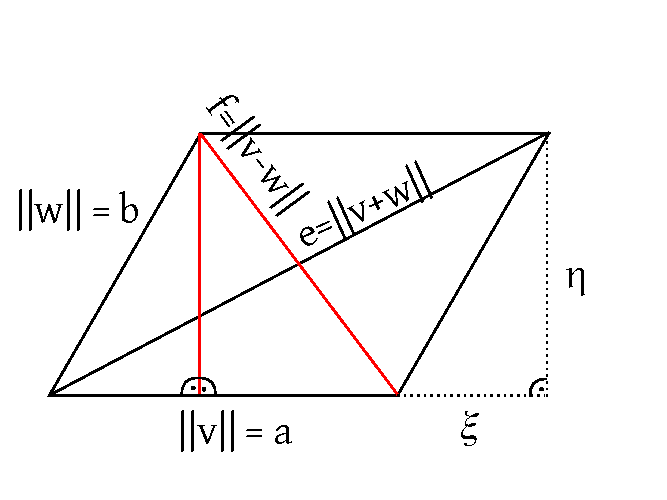
\includegraphics{img/06_geometrical_proof.pdf}
      \caption{Geometrical proof of Theorem~\ref{thm834}}
    \end{center}
  \end{figure}

  \[ e^2 + f^2 = 2 (a^2 + b^2) \]
  \[ e^2 = (a + \xi)^2 + \eta^2 \]
  \[ f^2 = (a - \xi)^2 + \eta^2 \]
  \[ e^2 + f^2 = (a + \xi)^2 + (a - \xi)^2 + 2\eta^2 \]
  \[ = a^2 + \xi^2 + a^2 + \xi^2 + 2\eta^2 = 2a^2 + 2b^2 \]
\end{theorem}

\begin{proof}
  \begin{enumerate}
    \item 
      \begin{align*}
        \norm{v + w}^2 &= \ip{v + w}{v + w} = \ip vv + \ip vw + \ip wv + \ip ww \\
          &= \norm{v}^2 + \ip vw + \overline{\ip vw} + \norm{w}^2 \\
          &= \norm{v}^2 + 2 \underbrace{\Re\ip vw}_{\cos\varphi \cdot \norm v \cdot \norm w} + \norm{w}^2
      \end{align*}
    \item immediate, $\ip vw = 0$
    \item
      \begin{align*}
        \norm{v + w}^2 + \norm{v - w}^2 &= {\norm v}^2 + \norm{w}^2 + 2 \Re\ip vw + \norm{v}^2 + \norm{-w}^2 + 2\Re\ip v{-w} \\
          &= 2 \norm{v}^2 + 2 \norm{w}^2 + 0
      \end{align*}
  \end{enumerate}
  Other norms:
  \[ \norm{\begin{bmatrix} x_1 \\ \vdots \\ x_n \end{bmatrix}}_1 = \sum_{1}^n \card{x_i} \]
  \[ \norm{\begin{bmatrix} x_1 \\ \vdots \\ x_n \end{bmatrix}}_\infty = \max \card{x_i} \]
\end{proof}

\begin{remark} % 8.35
  You can show (von Neumann did):
  A norm on $\mathbb R^n$ satisfies the Parallelogram Law
  iff $\exists$ a scalar product on $\mathbb R^n$ such that $\norm v = \sqrt{\ip vv}$
\end{remark}

\index{Orthonormal}
\index{Orthonormal basis}
\begin{definition} % 8.36
  Let $(v, \ip ,)$ be a vector space with scalar product.
  A family $(v_i)_{i \in I} \subseteq V$ is called
  \begin{description}
    \item[orthogonal] if $\forall i \neq j: \ip{v_i}{v_j} = 0$
    \item[orthonormal] if additionally $\norm{v_i} = 1 \forall i$ \\
      hence $\forall i,j: \ip{v_i}{v_j} = \delta_{ij}$
    \item[orthonormal basis] if they are orthonormal and give a basis of $V$.
  \end{description}
\end{definition}

\begin{example} % 8.37
  \begin{enumerate}
    \item Canonical basis in $\mathbb R^n$ in regards of the standard scalar product
      \[ \ip{e_i}{e_j} = \delta_{ij} \]
    \item Fourier $\set{\sqrt 2 \sin{2\pi x}, \sqrt2 \sin{4\pi x}, \ldots, \sqrt2 \sin(2k \pi x), \ldots}$ with $k \in \mathbb N$
      union with $\set{\sqrt2 \cos{2\pi x}, \sqrt2 \cos{4\pi x}, \ldots} \cup \set{\mathfrak 1}$
      on $C[0,1]$.
      \[ \ip fg = \int_0^1 f(x) g(x) \, dx \]
      And this is wrong unless we redefine the term basis (not every function is built using the sine/cosine).
      A basis here is every function:
      \[ f(x) = \sum_{k=0}^\infty a_k \cos{2k \pi x} + \sum_{k=1}^\infty b_k \sin{2k \pi 2} \]
      And this is wrong as well unless we define equality more precisely (in the usual sense, it is wrong).
      Lebesgue did this later.
  \end{enumerate}
\end{example}

\begin{remark}
  For JPEG compression, Fourier transformation is applied. Hence, we consider
  the music (amplitudes) as $f$ and
  \[ f(x) = \sum_{k=0}^n a_k \cos{2k \pi x} + \sum_{k=1}^n b_k \sin{2k \pi 2} \]
  with $n$ finite.
\end{remark}

\begin{theorem} % 8.38
  \label{thm838}
  Let $(v_i){i \in I} \subseteq V$, $v_i \neq 0 \forall i$
  \begin{enumerate}
    \item $(v_i)_{i \in I}$ orthogonal $\iff \left(\frac{v_i}{\norm{v_i}}\right)_{i \in I}$ is orthonormal
    \item $(v_i)_{i \in I}$ is orthogonal, then $(v_i)_{i \in I}$ is linear independent.
  \end{enumerate}
\end{theorem}

\dateref{2018/04/18}

\[ \cos\varphi = \frac{\ip vw}{\norm{v} \norm{w}} \]
\[ v \bot w \iff \ip vw = 0 \]
$(v_i)_{i \in I}$ orthogonal if $\ip{v_i}{v_j} = 0 \forall i \neq j$ \\
orthonormal: $\ip{v_i}{v_j} = \delta_{ij}$.

\begin{proof}[Proof of Theorem~\ref{thm838}]
  Let $\sum_{k=1}^n \lambda_k v_{i_k} = 0$.
  \[ \implies 0 = \angel{\sum_{k=1}^n \lambda \cdot v_{i_k}, v_i} = \sum_{k=1}^n \lambda_k \angel{v_{i_k}, v_i} \]
  $\forall l \in \set{1, \ldots, n}:$ Let $i = i_l$.
  \[ i_l = \sum_{k=1}^n \lambda_k \angel{\underbrace{v_{i_k}, v_{i_l}}_{= \begin{cases} 0 & i_k \neq i_l \\ \norm{v_{i_l}}^2 & i_k = i_l \end{cases}} } \]
  \[ = \lambda_l \cdot \norm{v_{i_l}}^2 \implies \lambda_l = 0 \]
\end{proof}

\begin{theorem} % 8.39
  Let $B = (b_1, \ldots, b_n)$ is an orthonormalbasis of an finite dimensional vector space over $\mathbb K$.
  For $v \in V$, let $\Phi_B(v) = \begin{pmatrix} \lambda_1 \\ \vdots \\ \lambda_n \end{pmatrix}$.
  For $w \in V$, let $\Phi_B(w) = \begin{pmatrix} \mu_1 \\ \vdots \\ \mu_n \end{pmatrix}$.
  \begin{enumerate}
    \item $\lambda_i = \ip{v}{b_i}$
    \item $\ip vw = \sum_{i=1}^n \lambda_i \overline{\mu_i}$
  \end{enumerate}
\end{theorem}

\begin{proof}
  \begin{enumerate}
    \item
      \begin{align*}
        \ip{v}{b_i} &= \ip{\sum_{j=1}^n \lambda_j b_j}{b_i} \\
                    &= \sum_{j=1}^n \lambda_j \cdot \underbrace{\ip{b_j}{b_i}}_{= \delta_{ji}} \\
                    &= \lambda_i
      \end{align*}
    \item
      \begin{align*}
        \ip vw &= \ip{\sum_{i=1}^n \lambda_i b_i}{\sum_{j=1}^n \mu_j b_j} \\
               &= \sum_{i=1}^n \lambda_i \sum_{j=1}^n \overline{\mu_j} \underbrace{\ip{b_i}{b_j}}_{\delta_{ij}} \\
               &= \sum_{i=1}^n \lambda_i \cdot \overline{\mu_i}
      \end{align*}
      Compare: $B$ is an arbitrary basis:
      \[ \ip vw = \Phi_B(v)^T \cdot A \cdot \overline{\Phi_B(w)} \]
      \[ a_{ij} = \ip{b_i, b_j} = \delta_{ij} \]
      \[ A = I \]
      \[ \to \ip vw = \Phi_B(v)^T \cdot \overline{\Phi_B(w)} \]
  \end{enumerate}
\end{proof}

\index{Orthogonal complement}
\begin{definition}
  Let $V$ be a vector space with a scalar product.
  Let $v \in V$, then
  \[ v^\bot = \setdef{w \in V}{\ip vw = 0} \]
  For $M \subseteq V: M^\bot = \setdef{w \in V}{\forall u \in M: \ip uw = 0}$
  is called \emph{orthogonal complement of $v$} or \emph{orthogonal complement of $M$}
\end{definition}

Compare with Figure~\ref{orthocomp}
\begin{figure}[!h]
  \begin{center}
    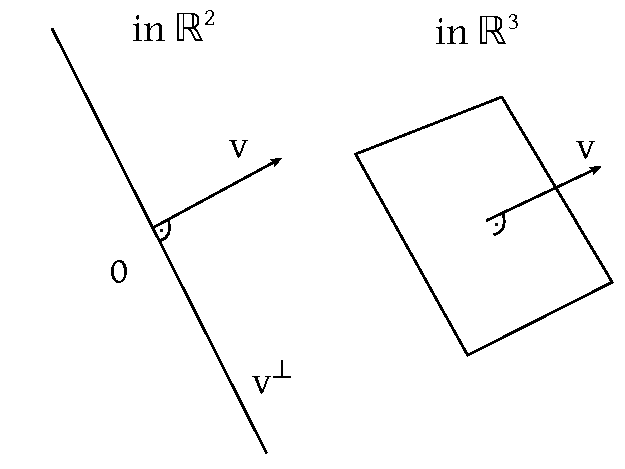
\includegraphics{img/07_orthogonal_complement.pdf}
    \caption{Orthogonal complement}
    \label{orthocomp}
  \end{center}
\end{figure}

in $\mathbb R^n$:
\[ \setdef{w}{\ip vw = 0} \]
\[ = \setdef{\begin{pmatrix} x_1 \\ \vdots \\ x_n \end{pmatrix}}{\sum_{1}^n a_i x_i = 0} \]
if $v = \begin{pmatrix} a_1 \\ \vdots \\ a_n \end{pmatrix}$.

\begin{theorem} % Theorem 8.41
  \label{thm841}
  Let $V$ be a vector with scalar product. $M, N \subseteq V$ are partitions.
  \begin{enumerate}
    \item $M^\bot$ is a subspace.
    \item $M \subseteq N \implies N^\bot \subseteq M^\bot$ \\
      $(M_1 \cup M_2)^\bot = M_1^\bot \cap M_2^\bot$
    \item $\set{0}^\bot = V$
    \item $V^\bot = \set{0}$
    \item $M \cap M^\bot \subseteq \set{0}$
    \item $M^\bot = \mathcal L(M)^\bot$
    \item $M \subseteq (M^\bot)^\bot$
  \end{enumerate}
\end{theorem}

\begin{proof}
  \begin{enumerate}
    \item
      \begin{align*}
        v^\bot &= \setdef{w \in V}{\ip vw = 0} \\
          T_v: & V \to \mathbb K \text{ (linear functional)} \\
               & w \mapsto \ip wv
      \end{align*}
      \[ v^\bot = \setdef{w}{T_v(w) = 0} = \ker{T_v} \]
      is a subspace.
      % the kernel of a linear map is a subspace
      \begin{align*}
        M^\bot &= \bigcap_{v \in M} v^\bot \\
               &= \bigcap_{v \in M} \ker(T_v)
      \end{align*}
      is a subspace.
    \item
      $M \subseteq N \implies N^\bot \subseteq M^\bot$
      \begin{align*}
        (M_1 \cup M_2)^\bot
          &= \setdef{w}{\forall v \in M_1: \ip wv = 0 \land \forall v \in M_2: \ip wv = 0} \\
          &= M_1^\bot \cap M_2^\bot
      \end{align*}
    \item trivial: $\forall v \in V: \ip v0 = 0$
    \item Let $w \in V$ such that $\ip wv = 0 \forall v \in V$. Especially for $v = w$.
      \[ \implies \underbrace{\ip ww}_{\norm{w}^2} = 0 \implies w = 0 \]
      \[ \implies V^\bot = \set{0} \]
    \item
      Let $w \in M \cap M^\bot$, hence
      \begin{align*}
        \forall v \in M: \ip wv &= 0 \\
        w \in M \implies \ip ww &= 0 \\
        \implies w &= 0 \\
        \text{or } M \cap M^\bot &= \varphi
      \end{align*}
    \item
      \[ M \subseteq \mathcal L(M) \underbrace{\implies}_{\text{by point (2.)}} \mathcal L(M)^\bot \subseteq M^\bot \]
      Show that: $M^\bot \subseteq \mathcal L(M)^\bot$.
      Hence, $\forall v \in M^\bot \implies v \in \mathcal L(M)^\bot$.
      Let $v \in M^\bot$, $w \in \mathcal L(M)$.
      \[
        \exists w_1, \ldots, w_n \in M: \exists \lambda_1, \ldots, \lambda_n \in \mathbb K:
        w = \sum_{i=1}^n \lambda_i w_i
      \]
      \begin{align*}
        \ip wv &= \ip{\sum_{i=1}^n \lambda_i w_i}{v} \\
               &\underbrace{=}_{\text{by linearity in 1st argument}} \sum_{i=1}^n \lambda_i \underbrace{\ip{\underbrace{w_i}_{\in M}}{\underbrace{v}_{\in M^\bot}}}_{= 0} = 0 \\
               & \implies v \bot w \quad \forall w \in \mathcal L(M)
      \end{align*}
    \item Show that $\forall v \in M: v \in (M^\bot)^\bot$. Hence, $\forall w \in M^\bot: v \bot w$
      \[ M^\bot = \setdef{w}{\forall v \in M: v \bot w} \]
      \[ \implies \forall v \in M \forall w \in M^\bot: v \bot w \implies \forall w \in M^\bot \forall v \in M, v \in W^\bot \]
      \[ \implies \forall v \in M: v \in \bigcap_{w \in M^\bot} w^\bot = (M^\bot)^\bot \]
  \end{enumerate}
\end{proof}

\begin{corollary} % Folgerung 8.42
  Let $U \subseteq V$ be a subspace.
  By Theorem~\ref{thm841} (1), $U^\bot$ is a subspace and $U \cap U^\bot = \set{0}$
  because of Theorem~\ref{thm841} (5),
  \[ U + U^\bot \text{ is direct sum} \]
  in $\mathbb R^n: U + U^\bot = \mathbb R^n$.
\end{corollary}

\begin{remark} % Bemerkung 8.43
  If $\dim(V) = \infty$, it must not hold that $U + U^\bot = V$.
  \begin{example}
    \[ V = l^2 = \setdef{(x_n)_{n \in \mathbb N}}{\sum \card{x_n}^2 < \infty} \]
    \begin{align*}
      U &= \mathcal L((e_i)_{i \in \mathbb N}) \\
        &= \setdef{(x_n)_{n \in \mathbb N}}{x_n = 0 \text{ except for finite many } n} \\
      U^\bot &= \setdef{e_i}{i \in \mathbb N}^\bot = \setdef{(x_n)_{n \in \mathbb N}}{\underbrace{\ip{(x_n)_{n \in \mathbb N}}{e_i}}_{= \setdef{(x_n)_{n \in \mathbb N}}{\forall i \in \mathbb N: x_i = 0} = \set{0}} = 0 \forall i \in \mathbb N} \\
      \ip{(x_n)_{n}}{(y_n)_{n}} &= \sum_{n=1}^\infty x_n \overline{y_n} \\
        &\implies U^\bot = \set{0} \\
        &\text{but } U + U^\bot \neq l_2
    \end{align*}
  \end{example}
\end{remark}

$U \dot{+} U^\bot$ is a direct sum.
\[ v \in U \dot{+} U^\bot \]
\[ U \xrightarrow{\pi_U} U \]
\[ U^\bot \xrightarrow{\pi_{U^\bot}} U^\bot \]
Every $v \in U \dot{+} U^\bot$ has a unique decomposition:
\[ v = u + w \qquad u \in U, w \in U^\bot \]

\begin{definition}
  Let $V$ be a vector space.
  A subset $K \subseteq V$ is called convex\footnote{Wide-sighted people with glasses use a glass with convex curvature.} if
  \[ \forall \lambda \in [0,1]: \forall x,y \in K: \lambda x + (1 - \lambda) y \in K \]
\end{definition}

\begin{example} % Example 8.45
  Subspaces are convex.
  \begin{enumerate}
    \item
      \[ U \subseteq V: \forall x, y \in U \forall \lambda, \mu: \lambda x + \mu y \in U \]
      Especially: $\lambda \in [0,1], \mu = 1 - \lambda$
    \item
      Let $(V, \norm{\cdot})$ be a normed space.
      \[ B_{\norm{\cdot}}(0,1) = \setdef{x \in V}{\underbrace{\norm{x} < 1}_{\text{unit circle}}} \]
      We discussed three different norms so far.
      In $\mathbb R^2$ with $\norm{\cdot}_2$ (Euclidean norm), the unit circle is a circle of radius $1$.
      In $\mathbb R^2$ with $\norm{\vectwo xy}_{\infty} = \max(\card{x}, \card{y})$ (infinity norm), the unit circle is a square from $(-1,-1)$ to $(1,1)$. This square contains the circle of radius $1$.
      In $\mathbb R^2$ with $\norm{\vectwo xy}_{1} = \card{x} + \card{y}$ (Manhattan norm),
      the unit circle is a square rotated by 45 degrees from $(-1, 0)$ to $(1, 0)$. It also contains the circle of radius $1$.

      Let $x, y \in B(0,1)$, hence $\norm{x} < 1$, $\norm{y} < 1$.
      \begin{align*}
        \norm{\lambda x + (1 - \lambda) y}
          &\underbrace{\leq}_{\text{by triangle ineq.}} \lambda \norm{x} + (1 - \lambda) \norm{y} \\
          &< \lambda + (1 - \lambda) \\
          &= 1 \\
          &\implies \lambda x + (1 - \lambda) y \in \mathcal B(0,1)
      \end{align*}
    \item
      Translation in a convex set gives a convex set.
      Let $K$ be convex. $K' = x_0 + K = \setdef{x_0 + z}{z \in K}$
      Let $x', y' \in K' \implies x' = x_0 + x$ and $y' = x_0 + y$.
      \begin{align*}
        \implies \lambda x' + (1 - \lambda) y' &= \lambda \cdot (x_0 + x) + (1 - \lambda)(x_0 + y) \\
          &= x_0 + \underbrace{\lambda x + (1 - \lambda) y}_{\in K}
      \end{align*}
      Especially: linear manifolds are convex.
      $B(x_0, 1)$ is convex.
    \item $K \subseteq V$ convex. $f: V \to W$ is linear. $\implies f(K)$ is convex.
  \end{enumerate}
\end{example}

Optimization: Given a set $M$ and a function $f: M \to \mathbb R$.
Find $y \in M$ such that $f(y)$ is minimal.

Find $y \in M$ such that $d(x_0, y)$ is minimal.
Compare with Figure~\ref{optprob}.

\begin{figure}[!h]
  \begin{center}
    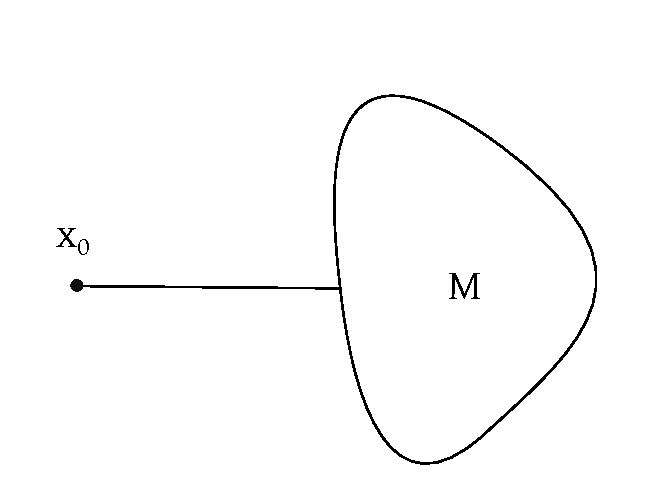
\includegraphics{img/08_generic_optimization_problem.pdf}
    \caption{A generic optimization problem}
    \label{optprob}
  \end{center}
\end{figure}

Now if $M$ is convex (consider $M$ convex in $(\mathbb R^n, \norm{\cdot}_2)$),
there exists a unique element $y \in M$ such that $\norm{x_0 - y}$ is minimal.

Finite elements (in computational mathematics) is the same idea.

\begin{theorem} % Satz 8.46
  $(V, \ip{\cdot}{\cdot})$ is a vector space with scalar product.
  $K \subseteq V$ is convex. Let $x \in V$ be given. Let $y_0 \in K$.
  Then the following statements are equivalent:
  \begin{enumerate}
    \item $\forall y \in K: \norm{x - y_0} \leq \norm{x - y}$
    \item $\forall y \in K: \Re\ip{x - y_0}{y - y_0} \leq 0$
    \item $\forall y \in K \setminus \set{y_0}: \norm{x - y_0} < \norm{x - y}$
  \end{enumerate}
  Compare with Figure~\ref{optconv}.
  In the special case if $K = U$ is a subspace, then the following statement is given (equivalent to statement~2)
  \begin{enumerate}
    \item[2'.] $\forall y \in U: \ip{x - y_0}{y - y_0} = 0$
  \end{enumerate}
\end{theorem}
\begin{figure}[!h]
  \begin{center}
    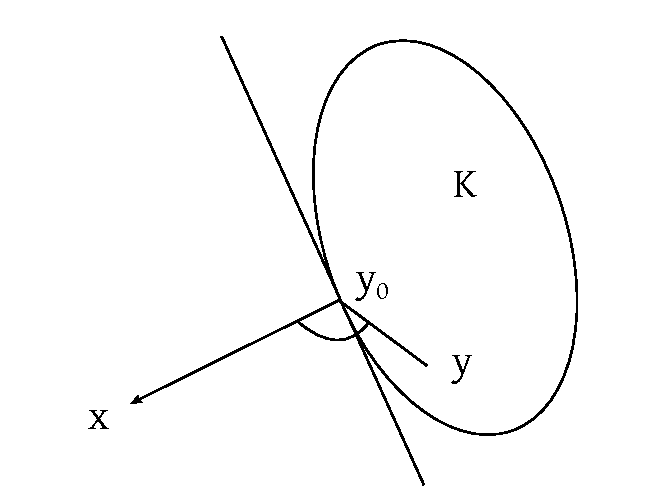
\includegraphics{img/09_optimization_on_a_convex_set.pdf}
    \caption{Optimization on a convex set}
    \label{optconv}
  \end{center}
\end{figure}

\begin{proof}
  \begin{enumerate}
    \item[1 $\to$ 2.]
      Let $y \in K: 1 > \varepsilon > 0$.
      \[ y_\varepsilon = \underbrace{y_0 + \varepsilon(y - y_0)}_{\varepsilon y + (1 - \varepsilon) y_0 \text{ because of convexity}} \in K \]
      \begin{align*}
        \forall \varepsilon in ]0,1[: \norm{x - y_0}^2
          &\leq \norm{x - y_{\varepsilon}}^2 \\
          &= \norm{x - (y_0 + \varepsilon (y - y_0))}^2 \\
          &= \norm{(x - y_0) - \varepsilon(y - y_0)}^2 \\
          &= \norm{x - y_0}^2 - 2\varepsilon\Re\ip{x - y_0}{y - y_0} + \varepsilon^2 \norm{y - y_0}^2 \\
       \implies \forall 0 < \varepsilon < 1: 0
          &\leq -2\varepsilon \Re\ip{x - y_0}{y - y_0} + \varepsilon^2 \norm{y - y_0}^2 \\
          &= \varepsilon \cdot \left(- 2\Re\ip{x - y_0}{y - y_0} + \varepsilon \norm{y - y_0}^2\right) \\
          &\underbrace{\implies}_{\varepsilon \to 0} 0 \leq - 2\Re\ip{x - y_0}{y - y_0}
      \end{align*}
    \item[2 $\to$ 3.]
      \begin{align*}
        \norm{x - y}^2 &= \norm{(x - y_0) + (y_0 - y)}^2 \\
          &= \norm{(x - y_0) - (y - y_0)}^2 \\
          &= \norm{x - y_0}^2 + \norm{y - y_0}^2 \underbrace{- 2\Re\ip{x - y_0}{y - y_0}}_{\geq 0} \\
          &\geq \norm{x - y_0}^2 + \norm{y - y_0}^2 \\
          &> \norm{x - y_0}^2 \\
          & y \neq y_0
      \end{align*}
    \item[3 $\to$ 1.]
      trivial.
    \item[2 $\to$ 2'.]
      Consider $K = U$ is subspace.
      \[ \forall y \in Y: \Re\ip{x - y_0}{y - y_0} \leq 0 \]
      $U$ is a subspace.
      \[ \setdef{y - y_0}{y \in U} = \setdef{z}{z \in U} = U - y_0 \]

      \[
        \left.
        \begin{array}{ll}
          \forall z \in U: &\Re\ip{x - y_0}{z} \leq 0 \\
          \forall z \in U: &\Re\ip{x - y_0}{-z} \leq 0
        \end{array}
        \right\}
        \implies \forall z \in U: \Re\ip{x - y_0}{z} = 0
      \]
      Case $K = \mathbb C$:
      \[ i \cdot U = U \]
      \[ \implies z \in U: \Re\ip{x - y_0}{iz} = 0 \]
      \[ \Re\overline{i}\ip{x - y_0}{z} = \Im\ip{x - y_0}{z} \]
  \end{enumerate}
\end{proof}

\begin{corollary}
  Let $(V, \angel{,})$ be a vector space.
  \begin{enumerate}
    \item $K \subseteq V$ is convex, $x \in V$.
      Then the optimization problem
      \[
        \left\{\begin{array}{c}
          \norm{x - y} = \min! \\
          y \in K
        \end{array}\right.
      \]
      has at most one solution.
    \item If $K = U$ subspace,
      then there exists at most one $y_0 \in U$ such that $x - y_0 \in U^\bot$.
  \end{enumerate}
\end{corollary}

\dateref{2018/04/23}

Orthonormalbasis:
\[ \ip{b_i}{b_j} = \delta_{ij} \]
\[ v = \sum \lambda_i b_i \leadsto \ip{v}{b_i} = \lambda_i \]
Given: an arbitrary basis of a subspace \\
Find: orthonormal basis of the subspace

TODO sketch drawing (projection and convexity)

\[ K \subseteq V \text{ convex} \]
$V$ with scalar product.

Then the optimization problem
\[ \norm{x - y} = \min \qquad Y \in K \]
has at most one solution.

$y$ is the solution.
\[ \iff \Re\ip{x-y_0}{y - y_0} \leq 0 \forall y \in K \]
If $K$ is the subspace $U$ ($x - y_0 \bot U$), then
\[ \Re\ip{x - y_0}{y} = 0 \forall y \in K \]

\[ U^\bot = \setdef{y}{y \bot U} \]
is subspace.
\[ U \cap U^\bot = \set{0} \]
If $x \in U \cap U^\bot$, then $x \bot x = \ip{x}{x} = \norm{x}^2 = 0$.

Orthogonal complement: $U + U^\bot$ is direct sum. \\
Every $x \in U + U^\bot$ has a unique decomposition.
\[ x = u + v \qquad u \in U, v \in U^\bot \]
The maps $x \mapsto u$ and $x \mapsto v$ are linear.

\begin{definition}
  Assume $U \dot+ U^\bot = V$.
  Then the projection maps
  \[ \pi_U: V \to V \qquad \pi_U: V \to V \]
  such that $\pi_U(x) \in U$ and $\pi_U(x) \in U^\bot$ and $x = \pi_U(x) + \pi_{U^\bot}(x)$ are orthogonality projections.
\end{definition}

\begin{remark}
  \begin{enumerate}
    \item $x \in U \iff \pi_U(x) = x \iff \pi_{U^\bot}(x) = 0$
    \item $x \in U^\bot \iff \pi_U(x) = 0 \iff \pi_{U^\bot}(x) = x$
    \item $\pi_{U^\bot} = \operatorname{id} - \pi_U$
  \end{enumerate}
\end{remark}

\[ \pi_U(x) \in U \]
\[ \implies \text{remark (4): } \pi_U(\pi_U(x)) = \pi_U(x) \]
\[ \text{($\sim$): } \pi_U \circ \pi_U = \pi_U \text{ idempotent} \]
\[ \pi_U \text{ is linear: } \pi_U \circ \pi_{U^\bot} = 0 \]

\begin{theorem} % 8.50
  Let $V = U \dot+ U^{\bot}$.
  \begin{enumerate}
    \item $\forall x, y \in V: \ip{x}{\pi_{U(y)}} = \ip{\pi_U(x)}{y} = \ip{\pi_U(x)}{\pi_U(y)}$
    \item Compare with Figure~\ref{img:proj}.
      \begin{figure}[!h]
        \begin{center}
          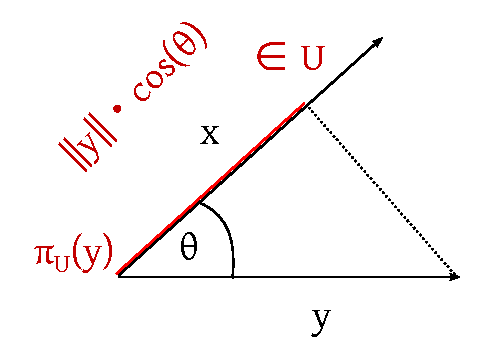
\includegraphics{img/10_projection.pdf}
          \caption{Projection}
          \label{img:proj}
        \end{center}
      \end{figure}
        \[ \norm{\pi_{u}(x)} \leq \norm{x} \land \norm{\pi_U(x)} = \norm{x} \iff x \in U \]
        Proof:
        \begin{enumerate}
          \item
            \[ x = \pi_U(x) + \pi_{U^\bot}(x) \qquad y = \pi_U(y) + \pi_{U^\bot}(y) \]
            \[ \ip{x}{\pi_U(y)} = \ip{\pi_U(x) + \pi_{U^\bot}(x)}{\pi_U(y)} = \ip{\pi_U(x)}{\pi_U(y)} + \underbrace{\ip{\underbrace{\pi_U(x)}_{\in U^\bot}}{\underbrace{\pi_U(y)}_{\in U}}}_{= 0} \]
            \[ \ip{\pi_U(x)}{y} = \ip{\pi_U(x)}{\pi_U(y)} + \ip{\pi_U(x)}{\pi_{U^\bot}(y)} \]
          \item
            \[ x = \pi_U(x) + \pi_{U^\bot}(x) \]
            \[ \implies \norm{x}^2 = \norm{\pi_U(x)}^2 + \norm{\pi_{U^\bot}(x)}^2 \geq \norm{\pi_U(x)}^2 \]
            By equality $\iff \norm{\pi_{U^\bot}(x)} = 0 \iff x = \pi_U(x) \iff x \in U$
        \end{enumerate}
  \end{enumerate}
\end{theorem}

\index{Gram matrix of tuple $v_1, v_2, \ldots, v_m$}
\begin{definition} % 8.51
  J{\o}rgen Pedison Gram (1850--1916)

  Let $v_1, v_2, \ldots \in V$.
  \[
    \operatorname{Gram}(v_1, \ldots, v_m) = \begin{bmatrix}
      \ip{v_1}{v_1} & \ip{v_1}{v_2} & \ldots & \ip{v_1}{v_m} \\ 
      \ip{v_2}{v_1} & \ip{v_2}{v_2} & \ldots & \ip{v_2}{v_m} \\ 
      \vdots & \vdots & \vdots & \vdots \\
      \ip{v_m}{v_1} & \ip{v_m}{v_2} & \ldots & \ip{v_m}{v_m}
    \end{bmatrix}
  \]
  is called \emph{Gram matrix of tuple $v_1, v_2, \ldots, v_m$}
\end{definition}

\begin{remark} % Bemerkung 8.52
  In case $V = \mathbb C^n$.
  \[ \ip vw = \overline{w}^T \cdot v = \sum_{1}^n \lambda_i \overline{\mu_i} = (\overline \mu_1, \ldots, \overline \mu_n)\begin{pmatrix} \lambda_1 \\ \vdots \\ \lambda_n \end{pmatrix} \]
  \[ v = \begin{pmatrix} \lambda_1 \\ \vdots \\ \lambda_n \end{pmatrix} \qquad w = \begin{pmatrix} \mu_1 \\ \vdots \\ \mu_n \end{pmatrix} \]
  Hence, if
  \[ v_i = \begin{pmatrix} \beta_{1i} \\ \vdots \\ \beta_{ni} \end{pmatrix} \qquad i = 1, \ldots, m \]

  \begin{align*}
    V &= \begin{pmatrix} v_1 & v_2 & \ldots & v_m \\ \vdots & \vdots & & \vdots \end{pmatrix} \in \mathbb C^{n \times m} \\
      &= \begin{pmatrix} \beta_{11} & \beta_{12} & \ldots & \beta_{1m} \\ \vdots & \vdots & & \vdots \\ \beta_{n1} & \beta_{n2} & \ldots & \beta_{nm} \end{pmatrix} \\
    (V^*V)_{ij} &= \sum_{k=1}^n (v^*)_{ik} v_{kj} = \sum_{k=1}^n \overline{\beta_{ki}} \beta_{kj} = \overline{\ip{v_i}{v_j}} \\
      &= \begin{pmatrix} v_1^* & \ldots \\ \vdots & \\ v_m^* & \ldots \end{pmatrix} \begin{pmatrix} v_1 & \ldots & v_m \\ \vdots &  & \vdots \end{pmatrix}
  \end{align*}
  \[ V^* V = \overline{\operatorname{Gram}(v_1, \ldots, v_m)} \]
\end{remark}

\begin{theorem} % 8.23
  Let $v_1, \ldots, v_m \in V$. $G = \operatorname{Gram}(v_1, \ldots, v_m)$.
  \begin{enumerate}
    \item $G = G^*$ is Hermitian, positive \emph{semi}definite.
      \[ \xi^T \cdot G \cdot \overline{\xi} = \norm{\sum_{i=1}^m \xi_i v_i}^2 \geq 0 \]
    \item $\xi \in \ker{G} \iff \sum_{i=1}^m \overline{\xi_i} v_i = 0$
    \item $G$ is positive definite iff $(v_1, \ldots, v_m)$ are linear independent.
  \end{enumerate}
\end{theorem}

\begin{proof}
  \begin{enumerate}
    \item $g_{ij} = \ip{v_i}{v_j} = \overline{\ip{v_j}{v_i}} = \overline{g_{ji}}$
      \[ \xi^T \cdot G \cdot \overline{\xi} = \sum_{i=1}^n \sum_{j=1}^n \xi_i g_{ij} \overline{\xi_j} = \sum_{i=1}^n \sum_{j=1}^n \xi_i \overline{\xi_j} \ip{v_i}{v_j} = \ip{\sum_{i=1}^n \xi_i v_i}{\sum_{j=1}^n \xi_j v_j} = \norm{\sum_{i=1}^n \xi_i v_i}^2 \]
    \item
      Direction $\implies$.
      $\xi \in \ker{G} \implies G \xi = 0 \implies \xi^T \cdot G \cdot \xi = 0$
      \[ \xi^T \cdot G \cdot \xi = \xi^T \cdot G \cdot \overline{\xi} \underbrace{=}_{(1)} \norm{\sum_{i=1}^m \overline{\xi_i} v_i}^2 \]
      Direction $\impliedby$. If $\norm{\sum_1^m \xi_i v_i} = 0$
      \[ (G \cdot \xi)_i = \sum_{j=1}^n \ip{v_i}{v_j} \xi_j = \sum_{j=1}^n \ip{v_i}{\overline{\xi_j} v_j} = \ip{v_i}{\underbrace{\sum_{j=1}^n \overline{\xi_j}}_{=0} v_j} = 0 \]
      \[ \implies G \cdot \xi = 0 \]
    \item $G$ is positive definite
      \begin{align*}
        &\iff \forall \xi \neq 0: \xi^T \cdot G \cdot \xi > 0 \\
        &\iff \forall \xi \neq 0: \norm{\sum_1^m \xi_i \cdot v_i}^2 > 0 \\
        &\iff \forall \xi \neq 0: \sum_{i=1}^m \xi_i v_i \neq 0 \\
        &\iff (v_1, \ldots, v_m) \text{ is linear independent} \\
        &\iff \ker{G} = \set{0} \\
        &\iff G \text{ is regular}
      \end{align*}
  \end{enumerate}
\end{proof}

\begin{theorem} % 8.54
  Let $U \subseteq V$ be a subspace. $V$ is a vector space with scalar product.
  \[ (u_1, \ldots, u_m) \text{ is basis of } U \]
  \[ G = \operatorname{Gram}(u_1, \ldots, u_m) = \left[\ip{u_i}{u_j}\right]_{i,j=1,\ldots,m} \]
  Then the projection $\pi_U(x) = \sum_{j=1}^m \eta_j u_j$ where
  \[ \eta = \overline{G}^{-1} \cdot \begin{pmatrix} \ip{x}{u_1} \\ \vdots \\ \ip{x}{u_m} \end{pmatrix} \]
  If $u_1, \ldots, u_m$ would be an orthonormal basis, then
  \[ \begin{pmatrix} \ip{x}{u_1} \\ \vdots \\ \ip{x}{u_m} \end{pmatrix} \]
  would be the coordinate of $x$.
\end{theorem}

\begin{figure}[t]
  \begin{center}
    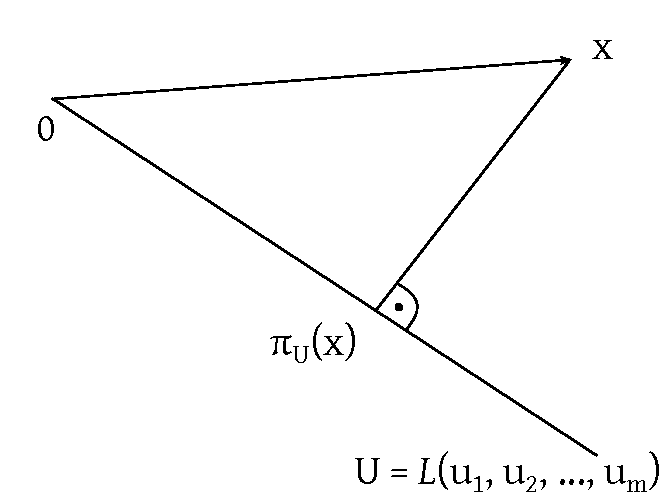
\includegraphics{img/11_projection.pdf}
    \caption{Projection}
    \label{img:projection}
  \end{center}
\end{figure}

Let $u = \sum_{j=1}^m \eta_j u_j$. Compare with Figure~\ref{img:projection}.
Show that $x - u \in U^{\bot} = \mathcal L(u_1, \ldots, u_m)^\bot = \set{u_1, \ldots, u_m}^\bot = \bigcap_{i=1}^m u_i^\bot$

Hence, show that $x - u \bot u_i \forall i \in \set{1, \ldots, m}$.

\begin{align*}
  \ip{u_i}{u} &= \ip{u_i}{\sum_{j=1}^m \eta_j u_j} \\
    &= \sum_{j=1}^m \ip{u_i}{u_j} \cdot \overline{\eta_j} \\
    &= \sum_{j=1}^m g_{ij} \overline{\eta_j} \\
    &= (G \overline{\eta})_i
    &= \ip{u_i}{x}
\end{align*}
because
\begin{align*}
  \overline G \cdot \eta &= \begin{pmatrix} \ip{x}{u_1} \\ \vdots \\ \ip{x}{u_m} \end{pmatrix} \\
  G \cdot \overline \eta &= \begin{pmatrix} \ip{x}{u_1} \\ \vdots \\ \overline{\ip{x}{u_m}} \end{pmatrix} = \begin{pmatrix} \ip{u_1}{x} \\ \vdots \\ \ip{u_m}{x} \end{pmatrix}
\end{align*}
Hence, $\forall i \in \set{1, \ldots, m}$:
\[ \ip{u_i}{u} = \ip{u_1}{x} \implies \forall i \in \set{1, \ldots, m}: \ip{u_i}{x - u} = 0 \implies x - u \in \set{u_1, \ldots, u_m}^\bot \]

\begin{example} % Beispiel 8.55
  \label{ex855}
  Find polynomial $p(t)$ of degree $2$ such that
  \[ \int_0^1 \card{t^3 - p(t)}^2 \, dt \overset!= \min \]
  $V = C[0,1]$, scalar product
  \[ \ip{f}{g} = \int_0^1 f(t) \overline{g(t)} \, dt \]
  \begin{align*}
    U &= \text{ polynomial function of degree } \leq 2 \\
    x &= t \mapsto t^3 \not\in U
  \end{align*}
  Find $p \in U$ such that $\norm{x - p}^2 \overset!= \min$
  \[ \norm{x - p}^2 = \int \card{x(t) - p(t)}^2 \, dt \]
  Basis of $U = \mathcal L(\set{1, t, t^2})$
  \[ u_i(t) = t^{i-1} \qquad i = 1,2,3 \]
  Gram matrix:
  \[ g_{ij} = \ip{u_i}{u_j} = \int_0^1 t^{i-1} t^{j-1} \, dt = \int_0^1 t^{i+j-2} \, dt = \left. \frac{t^{i+j-1}}{i + j - 1} \right|_0^1 = \frac{1}{i + j - 1} \]
  \[
    G = \begin{bmatrix}
      1 & \frac12 & \frac13 \\
      \frac12 & \frac13 & \frac14 \\
      \frac13 & \frac14 & \frac15
    \end{bmatrix}
  \]
  Hilbert matrix:
  \[ \left[\frac{1}{i+j-1}\right]_{i,j=1,\ldots,k} \]
  This matrix is very unstable (in the equation system $Gx = b$) and therefore a very important test matrix in computational mathematics (ie. Numerics).

  \[ u = \sum_{j=1}^3 \eta_j u_j \]
  \[ \eta = \overline{G}^{-1} \cdot \begin{pmatrix} \ip{x}{u_1} \\ \ip{x}{u_2} \\ \ip{x}{u_3} \end{pmatrix} \]
  \[ \ip{x}{u_j} = \int_0^1 x(t) u_j(t) \, dt = \int_0^1 t^3 \cdot t^{j-1} \, dt = \int_0^1 t^{2 + j} \, dt = \frac{1}{3 + j} \]
  \[
    \eta = \begin{bmatrix} 1 & \frac12 & \frac13 \\ \frac12 & \frac13 & \frac14 \\ \frac13 & \frac14 & \frac15 \end{bmatrix}^{-1}
    \begin{pmatrix} \frac14 \\ \frac15 \\ \frac16 \end{pmatrix}
    = \begin{bmatrix} 9 & -36 & 30 \\ -36 & 192 & -180 & 30 & -180 & 180 \end{bmatrix}
    \begin{bmatrix} \frac14 \\ \frac15 \\ \frac16 \end{bmatrix}
    = \begin{bmatrix} \frac1{20} \\ -\frac35 \\ \frac32 \end{bmatrix}
  \]
  (Assume that we don't know $180$ in the bottom-right corner precisely. Consider $180+\varepsilon$, then this error $\varepsilon$ explodes tremendously in the solution).
\end{example}

\begin{corollary} % 8.56
  \label{ONRcor}
  Special case $u_i$ is orthonormal basis of $U$ ($\rightarrow G = I$)
  Then it holds that
  \begin{enumerate}
    \item $\forall v \in V: \pi_U(v) = \sum_{i=1}^m \ip{v}{v_i} \cdot u_i$
    \item
      \[ \norm{v}^2 \geq \sum_{i=1}^m \card{\ip{v}{v_i}}^2 \qquad \text{ (Bessel's inequality)} \]
      \[ \norm{v}^2 = \sum_{i=1}^m \card{\ip{v}{u_i}}^2 \iff v \in U \qquad \text{ (Parseval's identity)} \]
      \[ \eta_j = \overline{G}^{-1}\begin{pmatrix} \ip{v}{u_1} \\ \vdots \\ \ip{v}{u_m} \end{pmatrix} \]
      F. Bessel (1784--1846) \\
      M. A. Parseval (1755--1836)
  \end{enumerate}
\end{corollary}

\begin{proof}
  Gram's matrix = $I$.
  \[ \eta_j = \ip{v}{u_j} \]
\end{proof}

\subsection{Gram-Schmidt process}

Given: $U = \mathcal L(v_1, \ldots, v_m)$ \\
Find: orthonormal basis of $U$.

\index{Gram-Schmidt process}
\begin{theorem}[Gram–Schmidt process for orthogonalization] % 8.57
  Let $(v_1, \ldots, v_m) \subseteq V$ be linear independent.
  Then $\exists u_1, \ldots, u_m$ is orthonormal basis of $\mathcal L(v_1, \ldots, v_m)$, specifically inductive
  \[ u_1 = \frac{v_1}{\norm{v_1}} \]
  and for $k = 2, \ldots, m$:
  \[ \tilde u_k = v_k - \sum_{j=1}^{k-1} \ip{v_k}{u_j} \cdot u_j \]
  \[ u_k = \frac{\tilde{u_k}}{\norm{u_k}} \]
  \begin{figure}[t]
    \begin{center}
      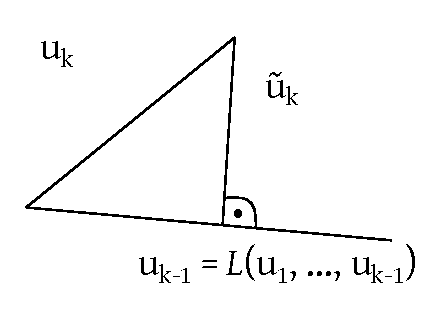
\includegraphics{img/12_GS_projection.pdf}
      \caption{Projection used in the Gram-Schmidt process}
      \label{GSproj}
    \end{center}
  \end{figure}
\end{theorem}

\begin{proof}
  \begin{description}
    \item[Induction base] $k=1$ is trivial
    \item[Induction step] $k-1 \to k$. Assume
      \[ \mathcal L(u_1, \ldots, u_{k-1}) = \mathcal L(v_1, \ldots, v_{k-1}) \eqqcolon U_{k-1} \]
      \[ \tilde u_k = v_k - \pi_{U_{k-1}}(v_k) \in U_{k-1}^\bot \text{ because of Theorem~\ref{ONRcor}} \]
      \[ \implies \tilde u_k \bot u_1, \ldots, u_{k-1} \implies (u_1, \ldots, u_{k-1}, \frac{\tilde u_k}{\norm{\tilde u_k}}) \]
      is an orthonormal basis.
      \[
        \mathcal L(u_1, \ldots, u_{n-1}, \frac{\tilde u_k}{\norm{\tilde u_k}})
          = \mathcal L(u_1, \ldots, u_{k-1}, v_k)
      \]
      then $\tilde u_k - v_k \in \mathcal L(u_1, \ldots, u_{k-1})$
  \end{description}
\end{proof}

\dateref{2018/04/25}

Gram-Schmidt process:
\[ \mathcal L(v_1, v_2) = \mathcal L(v_2 - p(v_2), v_1) \qquad v_2 - p(v_2) \bot v_1 \]

Given: $v_1, \ldots, v_m$
\[ u_i = \frac{v_i}{\norm{v_i}} \]
\[ \tilde u_k = v_k - \sum_{i=1}^{k-1} \ip{v_k}{u_i} \cdot u_i \]
\[ u_k = \frac{\tilde u_k}{\norm{\tilde u_k}} \qquad \frac{\ip{v_k}{\tilde u_i} \tilde u_i}{\norm{\tilde u_i}^2} \]

\begin{example}
  Let $V = \mathbb R^3$.
  \[ \ip xy = x^t A y \]
  \[
    A = \begin{bmatrix}
      1 & -1 & 1 \\
      -1 & 3 & -1 \\
      1 & -1 & 2
    \end{bmatrix}
  \]
  \[ v_i = \text{ standard basis } e_i \]
  \[ \norm{v_1}^2 = \ip{v_1}{v_1} = v_1^T A v_1 = a_{11} = 1 \]
  \[ \norm{v_2}^2 = \ip{v_2}{v_2} = a_{12} = 3 \]
  \[ u_1 = \frac{v_1}{\norm{v_1}} = \begin{pmatrix} 1 \\ 0 \\ 0 \end{pmatrix} \]
  \[ \tilde u_2 = v_2 - u_1 \ip{v_2}{u_1} = \begin{pmatrix} 0 \\ 1 \\ 0 \end{pmatrix} - \begin{pmatrix} 1 \\ 0 \\ 0 \end{pmatrix} \cdot (0 \: 1 \: 0) A \begin{pmatrix} 1 \\ 0 \\ 0 \end{pmatrix} = \begin{pmatrix} 0 \\ 1 \\ 0 \end{pmatrix} + \begin{pmatrix} 1 \\ 0 \\ 0 \end{pmatrix} = \begin{pmatrix} 1 \\ 1 \\ 0 \end{pmatrix} \]
  \[ u_2 = \frac{\tilde u_2}{\norm{\tilde u_2}} \qquad \norm{\tilde u_2}^2 = \ip{\tilde u_2}{\tilde u_2} = (1 \: 1 \: 0) \cdot A \begin{pmatrix} 1 \\ 1 \\ 0 \end{pmatrix} = 2 \qquad u_2 = \frac{1}{\sqrt2} \begin{pmatrix} 1 \\ 1 \\ 0 \end{pmatrix} \]
  \[ \tilde u_3 = v_3 - u_1 \ip{v_3}{u_1} - u_2 \ip{v_3}{u_2} \]
  \[ = \begin{pmatrix} 0 \\ 0 \\ 1 \end{pmatrix} - \vecthree100 \cdot \underbrace{(0 \: 0 \: 1) \cdot A \cdot \vecthree100}_{a_{31} = 1} - \frac{1}{\sqrt{2}} \vecthree110 \cdot \underbrace{(0 \: 0 \: 1) \cdot A \cdot \vecthree110}_{a_{31} + a_{32} = 0} \cdot \frac{1}{\sqrt2} = \vecthree{-1}01 \]
  \[ \norm{\tilde u_3}^2 = (-1 \: 0 \: 1) \cdot A \cdot \vecthree{-1}{0}1 = 1 - 1 - 1 + 2 = 1 \qquad u_3 = \vecthree{-1}{0}{1} \]
\end{example}

\begin{remark} % 8.59
  This is an alternative method to build orthogonal projection on subspace $U \subseteq \mathbb C^n$ with standard scalar product.
  \begin{enumerate}
    \item Determine an orthonormal basis of $U$: $u_1, \ldots, u_m \in \mathbb C^{n\times 1}$
    \item $P = \sum_{i=1}^m u_1 \cdot u_i^*$
  \end{enumerate}
  \[ P \cdot v = \sum_{i=1}^m u_i \underbrace{u_i^* \cdot v}_{\ip{v}{v_i}} = \sum_{i=1}^m u_i \ip{v}{v_i} \]
  Gram matrix = $I$
\end{remark}

\begin{example}[Example~\ref{ex855} again] % 8.60
  \[ V = C[0,1] \qquad U = \mathcal L(1, x, x^2) \eqqcolon \mathcal L(v_1, v_2, v_3) \]
  \[ \ip fg = \int_0^1 f(t) \overline{g(t)} \, dt \]
  Orthonormal basis:
  \[ \norm{v_i}^2 = \int_0^1 1^2 \, dt = 1 \]
  \[ u_1 = 1 \]
  \[ \tilde u_2 = v_2 - u_1 \cdot \ip{v_2}{u_1} = x - 1 \cdot \underbrace{\int_0^1 t \cdot 1 \, dt}_{= \frac12} = x - \frac12 \]
  \[ \norm{\tilde u_2}^2 = \int_0^1 (t - \frac12)^2 \, dt = \left.\frac{(t - \frac12)^3}{3} \right|_0^1 = \frac{(\frac12)^3 - (-\frac12)^2}{3} = \frac1{12} \]
  \[ u_2 = \frac{\tilde u_2}{\norm{\tilde u_2}} = \sqrt{12} \cdot (x - \frac12) \]
  \begin{align*}
    \tilde u_3 &= v_3 - u_1 \ip{v_3}{u_1} - u_2 \cdot \ip{v_3}{u_2} \\
      &= x^2 - 1 \cdot \underbrace{\int_0^1 t^2 \cdot 1 \, dt}_{= \frac13} - \sqrt{12} (x - \frac12) \int_0^1 t^2 \sqrt{12} (t - \frac12) \, dt \\
      &= x^2 - \frac13 - 12 (x - \frac12) \cdot \frac1{12} \\
      &= x^2 - x + \frac16
  \end{align*}
  Side note:
  \[ \int_0^1 t^2 (t - \frac12) \, dt = \int_0^1 (t^3 - \frac12 t^2) \, dt = \frac14 - \frac16 = \frac1{12} \]
  \[ \norm{\tilde u_3}^2 = \int_0^1 (t^2 - t + \frac16)^2 \, dt = \frac1{180} \]
  \[ \implies u_3 = \sqrt{180} \cdot (x^2 - x + \frac16) \]

  Projection:
  \[ \int_0^1 (t^3 - p(t))^2 \, dt = \operatorname{min}! \]
  Solution: $\pi_U(x^3) \qquad U = \mathcal L(1, x, x^2)$
  \begin{align*}
    \pi_U(x^3) &= u_1 \ip{x^3}{u_1} + u_2 \ip{x^3}{u_2} + u_3 \ip{x^3}{u_3} \\
      &= 1 \cdot \int_0^1  t^3 \cdot 1 \, dt + \sqrt{12} (x - \frac12) \int_0^1 t^3 \sqrt{12} (t - \frac12) \, dt \\
      &+ \sqrt{180} (x^2 - x + \frac16) \int_0^1 t^3 \sqrt{180} (t^2 - t + \frac16) \, dt
  \end{align*}
\end{example}

\index{Chebyshev polynomials}
Consider $\ip fg \coloneqq \int_{-1}^1 \sqrt{1 - t^2} f(t) \overline{g(t)} \, dt$.
Take $1, x, x^2, \ldots$ and apply Gram schmidt process to retrieve the Chebyshev polynomials.

\[ \int_0^1 f(t) g(t) \, dt \qquad \text{ Laguerre} \]
\[ \frac1{\sqrt{2\pi}} \int_{-\infty}^\infty e^{-\frac{t^2}{2}}  f(t) g(t) \, dt \qquad \text{ Hermite polynomials} \]

\subsection{Riesz representation theorem}

Frigyes Riesz (1880--1956)

Let $(V, \ip{\cdot}{\cdot})$ be a vector space with scalar product $\dim{V} < \infty$.

$V^*$ is the dual space $= \operatorname{Hom}(V, \mathbb K) = $ space of linear functionals.
For fixed $y \in V$ the map $T_y(x) = \ip{x}{y}$ is linear in $x$, hence $T_y \in V^*$.

Then the map $V \to V^*$ with $y \mapsto Ty: V \to \mathbb K$ with $x \mapsto \ip xy$ is an antilinear isomorphism (antiisomorphism).

This is trivial in $\mathbb R$, but in $\mathbb C$ is much more complex (pun intended).

Hence,
\begin{enumerate}
  \item For every $y$ it holds that $Ty \in V^*$
  \item For every linear functional $f \in V^*$
    \[ \exists! y \in V: f = T_y \]
  \item Let $y \mapsto Ty$ is an antilinear map.
    \[ T_{\lambda y_1 + \mu y_2} = \overline{\lambda} Ty_1 + \overline{\mu} Ty_2 \]
\end{enumerate}

\begin{example}[For point 2]
  \[ V = C[0,1] \]
  Scalar product: $\ip fg = \int f(t) g(t) \, dt$.
  Let $F: C[0,1] \to \mathbb R$ linear.
  Then by the Riesz representation theorem,
  there exists $g \in C[0,1]: F(f) = \int f(t) g(t) \, dt$.

  For example $f \to f(1)$
  \[ \exists g(t): f(1) = \int_0^1 f(t) g(t) \, dt \]
  In physics, e.g. the Dirac delta function.
\end{example}

\begin{proof}[Proof of point 3]
  We show linearity.

  \[ Ty(x) = \ip xy \text{ is linear in } X \implies T_y \in V^* \]
  \begin{align*}
    \forall x \in V: T_{\lambda y_1 + \mu y_2}(x)
      &= \ip{x}{\lambda y_1 + \mu y_2} = \overline{\lambda} \ip{x}{y_1} + \overline{\mu}\ip{x}{y_2} \\
      &= \overline{\lambda} Ty_1(x) + \overline{\mu} Ty_2(x) = (\overline{\lambda} Ty_1 + \overline{\mu} Ty_2)(x) \\
      &\implies T_{\lambda y_1 + \mu y_2} = \overline{\lambda} Ty_1 + \overline{\mu} Ty_2
  \end{align*}
  
  We show injectivity: the map $y \mapsto Ty$ is injective.

  Assume: $Ty = 0$ (zero functional). Show $y = 0$.
  $Ty = 0$ means $\forall x \in V: Ty(x) = 0$, especially for $x = y$, $T_y(y) = \ip yy = 0 \implies y = 0$.

  We show surjectivity: the map $y \mapsto Ty$ is surjective.

  Let $u_1, \ldots, u_n$ is an orthonormal basis (exists because of Gram-Schmidt).
  
  Given: $f \in V^*$.
  Find: $y$ such that $f = Ty$.
  \[ \text{Hence, } \forall x \in V: f(x) = \ip xy \underbrace{\iff}_{\text{by \foreignlanguage{german}{Fortsetzungssatz}}} f(u_i) = \ip{u_i}{y} \]
  Let $y = \sum_{j=1}^n \overline{f(u_j)} \cdot u_j$.
  \[ \implies \ip{u_i}{y} = \ip{u_1}{\sum_{j=1}^n \overline{f(u_j)} u_j} = \sum_{j=1}^n f(u_j) \underbrace{\ip{u_i}{u_j}}_{\delta_{ij}} = f(u_i) \]
  Hence, $y$ satisfies the condition.
\end{proof}

\begin{remark}
  The Riesz representation theorem also holds in infinite dimensions in the case of Hilbert spaces.
  In those spaces, there exists some Hilbert base:
  \[ (u_i)_{i \in I}: x = \sum_{i \in I} \ip x{u_i} \cdot u_i \forall x \]
  So every $x$ has such a representation and in infinite dimensions, this representation is a series.
\end{remark}

\begin{corollary} % Folgerungen 8.62
  \begin{enumerate}
    \item $v = 0 \iff \forall w \in V: \ip vw = 0$
    \item $\norm{v} = \sup\setdef{\card{\ip vw}}{\norm{w} \leq 1}$
  \end{enumerate}
  Equivalently in the dual space:
  \begin{enumerate}
    \item $v = 0 \iff \forall f \in V^*: f(v) = 0$
    \item $\norm{v} = \sup\setdef{\card{f(v)}}{f \in V^* \quad \norm{f} \leq 1}$
  \end{enumerate}
  holds in general in a normed space.
\end{corollary}

\begin{remark}
  We make a small revision: dual space $V^* = \operatorname{Hom}(V, \mathbb K)$
  \[ W \xrightarrow{T} V \xrightarrow{f} \mathbb K \]
  \[ \implies f \circ T: W \to \mathbb K \in W^* \]
  is a linear functional on $W$.
  Hence, the map $\operatorname{Hom}(V, \mathbb K) \to \operatorname{Hom}(W, \mathbb K)$ and $f \mapsto f \cdot T$ is linear.
  \[ (\lambda f + \mu g) \circ T = \lambda \cdot f_0 T + \mu g \circ T \qquad \text{\enquote{transposed map}} \]
  Linear map: $T^*: V^* \to W^*$.

  Let $V$, $W$ be spaces with a scalar product. Then $V \simeq V^*$ and $W \simeq W^*$ where $\simeq$ means anti-isomorphic.
  $T: W \to V \implies T^*: V \to W$.
\end{remark}

\index{Adjoint map}
\begin{definition}[Theorem and definition] % 8.63
  \label{def863}
  Let $(V, \ip{}{}_V)$ and $(W, \ip{}{}_W)$ be spaces with a scalar product. $\dim{V}, \dim{W} < \infty$.
  \[ T \in \operatorname{Hom}(W, V) \text{ hence, } T: W \to V \text{ linear} \]
  \begin{enumerate}
    \item For every $v \in V$ is the map
      \[ w \mapsto \ip{T(w)}{v}_V \qquad \text{ linear} \]
    \item $\forall v \in V \exists! u \in W \forall w \in W: \ip{T(w)}{v}_V = \ip{w}{u}_W$ and $T^*(v) = u$.
  \end{enumerate}
  Hence,
  \[ \ip{T(w)}{v}_V = \ip{w}{T^*(v)}_W \qquad \forall w \in W \quad \forall v \in V \]
  \begin{enumerate}
    \item[3.] The map $T^*: V \to W$ with $v \mapsto u$ is linear, hence $T^* \in \operatorname{Hom}(V, W)$ and is called \emph{adjoint map}.
    \item[4.] The map $\operatorname{Hom}(W, V) \mapsto \operatorname{Hom}(V, W)$ with $T \mapsto T^*$ is antilinear and $T^{**} = T$.
  \end{enumerate}
\end{definition}

\begin{proof}
  \begin{enumerate}
    \item $\ip{T(w)}{v} = T_V(T(w)) = T_v \circ T(w)$ \\
      Composition of linear maps is linear.
    \item $T_V \circ T \in W^*$. By Riesz representation theorem, $\exists! u \in W: T_V \circ T(w) = \ip{w}{u} \forall w \in W = \ip{T(w)}{v} = \ip wu$
    \item Show that,
      \[ \forall v_1, v_2 \in V \forall \lambda, \mu: T^*(\lambda v_1 + \mu v_2) = \lambda T^*(v_1) + \mu T^*(v_2) \]
      It suffices to show that
      \[ \ip{w}{T^*(\lambda v_1 + \mu v_2)} = \ip{w}{\lambda T^*(v_1) + \mu T^*(v_2)} \forall w \in W \]
      Compare with corollary: $w_1 = w_2$ in $W \iff \forall w: \ip{w}{w_1} = \ip{w}{w_2}$.
      \begin{align*}
        \ip{w}{T^*(\lambda v_1 + \mu v_2)} &= \ip{T(w)}{\lambda v_1 + \mu v_2} \\
          &= \overline{\lambda} \ip{T(w)}{v_1} + \overline{\mu} \ip{T(w)}{v_2} \\
          &= \overline{\lambda} \ip{w}{T^*(v_1)} + \overline{\mu} \ip{w}{T^*(v_2)} \\
          &= \ip{w}{\lambda T^*(v_1)} + \ip{w}{\mu T^*(v_2)} \\
          &= \ip{w}{\lambda T^*(v_1) + \mu T^*(v_2)}
      \end{align*}
    \item Show $(\lambda T_1 + \mu T_2)^* = \overline{\lambda} T_1^* + \overline{\mu} T_2^*$. \\
      \[ \iff \forall v \in V: (\lambda T_1 + \mu T_2)^* v = (\overline{\lambda} T_1^* + \overline{\mu} T_2^*)(v) \]
      \[ \forall v \in V \forall w \in W: \ip{w}{(\lambda T_1 + \mu T_2)^*(v)} = \ip{w}{(\overline{\lambda} T_1^* + \overline{\mu} T_2^*)(v)} \]
      Hence,
      \begin{align*}
        \ip{w}{(\lambda T_1 + \mu T_2)^*(v)}
          &= \ip{(\lambda T_1 + \mu T_2)(w)}{v} \\
          &= \lambda \ip{T_1(w)}{v} + \mu\ip{T_2(w)}{v} \\
          &= \lambda \ip{w}{T_1^*(v)} + \mu \ip{w}{T_2^*(v)} \\
          &= \ip{w}{\overline{\lambda} T_1^*(v)} + \ip{w}{\overline{\mu} T_2^*(v)} \\
          &= \ip{w}{\overline{\lambda} T_1^*(v) + \overline{\mu} T_2^*(v)} \\
          &= \ip{w}{(\overline\lambda T_1^* + \overline\mu T_2^*)(v)}
      \end{align*}

      \[ T: W \to V \qquad T^*: V \to W \qquad T^{**}: W \to V \]
      Show that $\forall w \in W: T^{**}(w) = T(w)$. Hence $\forall w \in W \forall v \in V: \ip{T^{**}(w)}{v}_V = \ip{T(w)}{v}_V$
      \begin{align*}
        \ip{T^{**}(w)}{v}_V &= \overline{\ip{v}{T^{**}(w)}} = \overline{\ip{T^*(v)}{v}} = \ip{w}{T^*(v)} \\
          &= \ip{T(w)}{v} \\
        \ip{Tw}{v} &= \ip{w}{T^*v}
      \end{align*}
      If $V = W$, then $T = T^*$.
    \item Assume $u = D^*(x)$ exists $\in \mathbb R[x]$ \\
      \[ \implies M \coloneqq \max_{t \in [0,1]} \card{u(t)} < \infty \]
      \[ \card{\card{x^n}{D^*(x)}} = \card{\int_0^1 t^n \cdot u(t) \, dt} \leq \int_0^1 t^n \cdot M \, dt = \frac{M}{n+1} \]
      \[ \implies \frac{n}{n+1} \leq \frac{M}{n+1} \forall n \in \mathbb N \]
      \[ \implies u(x) \not\in \mathbb R[x] \]
  \end{enumerate}
\end{proof}

\begin{example}[For Definition~\ref{def863}, point~3] % Beispiel 8.64
  If $\dim{V} = \infty$, then not every linear map has an adjoint map!
  \[ V = \mathbb R[x]_1 \]
  \[ \ip{f}{g} = \int_0^1 f(t) g'(t) \, dt \]
  \[ D: V \to V \qquad p(x) \mapsto p'(x) \]
  Recall: The derivative of a linear combination is the linear combination of derivatives.
  Assume $D$ has an adjoint $D^*$.
  \[ \implies \ip{x^n}{D^*(x)} = \ip{D(x^n)}{x} = \int_0^1 n t^{n-1} t \, dt = \frac{n}{n+1} \]
\end{example}

\dateref{2018/05/02}

\index{Involution}
Riesz representation theorem \\
$V$ with scalar product \\
$\operatorname{Hom}(V, \mathbb K) \simeq V$ where $\simeq$ is antilinear \\
$\forall f \in \operatorname{Hom}(V, \mathbb K): \exists! y \in V: f = T_y$ \\
\[ T_y(x) = \ip xy \]
\[ T_{\lambda x + \mu y} = \overline{\lambda} T_x + \overline\mu T_y \]
For $f \in \operatorname{Hom}(V, W)$, the map $x \mapsto \ip{f(x)}{y} \in \operatorname{Hom}(V, \mathbb K)$
\[ \implies \exists! z \in V: \forall x \in V: \ip{f(x)}{y} = \ip xz \]
\[ z \eqqcolon f^*(y) \text{ \dots adjoint map} \]
\[ f^*: W \to V \text{ is linear} \]
\[ \operatorname{Hom}(V, W) \to \operatorname{Hom}(W, V) \]
\[ f \mapsto f^* \]
is an antilinear \emph{involution}.
\[ f^{**} = f \]

\begin{theorem} % 8.65
  Let $B \subseteq V, C \subseteq W$ be orthonormal bases. $f \in \operatorname{Hom}(V, W)$.
  \[ \Phi_B^C(f^*) = \Phi_C^B(f)^* = \overline{\Phi_C^B(f)^T} \]
\end{theorem}

\begin{proof}
  \[ A = \Phi_C^B(f) \]
  Column $s_j(A)$ is the coordinate of $b_j \in B$ in regards of basis $C$.
  \begin{align*}
    a_{ij} &= \text{ i-th coordinate of } f(b_j) \\
      &= \Phi_C(f(b_j))_i = \ip{f(b_j)}{c_i} \\
      &= \ip{b_j}{f^*(c_i)} = \overline{\ip{f^*(c_i)}{b_j}} \\
      &= \text{ j-th coordinate of } f^*(c_i) \\
      &= \overline{\Phi_B^C(f^*)_{ji}} = \overline{\tilde{a}_{ji}}
  \end{align*}
  if $\tilde A = \Phi_B^C(f^*)$
\end{proof}

\begin{theorem} % 8.66
  Let $U, V, W$ be finite-dimensional.
  \[ U \xrightarrow f V \xrightarrow g W \]
  \begin{enumerate}
    \item $(g \circ f)^* = f^* \circ g^*$
    \item $f^{**} = f$
    \item $\ker{f} = (\im{f^*})^\bot$
    \item $\im{f} = (\ke{f^*})^\bot$
    \item $f$ injective $\iff f^*$ surjective
    \item $f$ surjective $\iff f^*$ injective
  \end{enumerate}
\end{theorem}
\begin{proof}
  \begin{enumerate}
    \item Let $u \in V, w \in W$
      \begin{align*}
        \ip{(g \circ f)(u)}{w}_W &= \ip{g(f(u))}{w}_W \\
          &= \ip{f(u)}{g^*(w)}_V \\
          &= \ip{u}{f^*(g^*(w))}_U
      \end{align*}
      holds $\forall u \in U \forall w \in W$. By definition
      \[ \ip{(g \circ f)(u)}{w}_W = \ip{u}{(g \circ f)^*(w)} \]
      Hence,
      \[ \implies (g \circ f)^* = f^* \circ g^* \]
    \item[3.] Show that
      \begin{itemize}
        \item $\ke{f} \subseteq (\im{f^*})^\bot$
        \item $(\im{f^*})^\bot \subseteq \ke{f}$
      \end{itemize}
      Proof:
      \begin{itemize}
        \item Let $u \in \ke{f}$. Show that $\forall y \in \im{f^*}: \ip uy = 0$
          \[ y \in \im{f^*} \implies \exists v \in V: y = f^*(v) \]
          \[ {\ip uy}_U = \ip{u}{f^*(v)}_U = \ip{\underbrace{f(u)}_{=0}}{v}_V = 0 \]
        \item Let $u \in (\im{f^*})^\bot$, hence $\forall v \in V: u \bot f^*(v)$.
          Hence $\forall v in V: \ip{u}{f^*(v)}_U = 0$.
          \[ \forall v \in V: \ip{f(u)}{v}_V = 0 \]
          \[ \implies f(u) \ in V^\bot = \set{0} \]
          \[ \implies u \in \ke{f} \]
      \end{itemize}
    \item[4.]
      Apply (3) to $f^*$.
      \[ \ke{f^*} = (\im{f^{**}})^\bot = (\im{f})^\bot \]
      \[ \implies \left(\ke{f^*}\right)^\bot = (\im{f})^{\bot\bot} \underbrace{=}_{\dim < \infty} \im{f} \]
  \end{enumerate}
\end{proof}

\begin{remark}[Addition to Theorem~\ref{thm841}]
  So, if subspace $U \subseteq V$. Then $U^{\bot\bot} = U$.

  Proof: It holds that $U \dot{+} U^\bot = V$ and $U^\bot \dot{+} U^{\bot\bot} = V$.
  $U \subseteq U^{\bot\bot}$ and $\dim{U} = \dim{U}^{\bot\bot} \implies U = U^{\bot\bot}$.
\end{remark}

\index{Self-adjoint map}
\index{Unitary transformation}
\index{Linear isometry}
\begin{definition} % 8.67
  Let $V$ be a vector space with scalar product.
  \begin{enumerate}
    \item $f: V \to V$ is called \emph{self-adjoint}, if $f = f^*$.
      Hence $\forall x, y \in V: \ip{f(x)}{y} = \ip{x}{f(y)} \iff \Phi_B^B(f) = \Phi_B^B(f)^*$
      if $B$ is orthonormal basis of $V$.
    \item
      $f \in \Hom(V,W)$ is called \emph{unitary transformation} or \emph{linear isometry} if
      \[ \forall x,y \in V: \ip{f(x)}{f(y)} = \ip{x}{y} \]
      esp. $\norm{f(x)} = \norm{x}$, hence lengths (and also angles) are preserved. \\
      \emph{mostly} it is additionally required that $f$ is invertible.
  \end{enumerate}
\end{definition}

\begin{remark} % Bemerkung 8.68
  \label{bem868}
  \begin{enumerate}
    \item Unitary transformations are injective.
    \item If $\dim{V} = \dim{W} < \infty$ and $f: V \to W$ is linear and unitary,
    then $f$ is regular and $f^{-1} = f^*$.
    \item If $\dim{V} = \infty$, $f: V \to V$ is isometry, it does not imply that $f$ is invertible.
  \end{enumerate}
\end{remark}

\begin{proof}
  \begin{enumerate}
    \item Immediate: $f(v) = 0 \implies \norm{f(v)} = \norm{v} = 0 \implies v = 0$
      \[ \ke{f} = \set{0} \]
    \item $f$ unitary $\xRightarrow{(1.)}$ $f$ injective $\implies$ $f$ surjective.
      \begin{align*}
        \forall x,y \in V: \ip xy &= \ip{f(x)}{f(y)} \\
          &= \ip{x}{f^* \circ f(y)}
      \end{align*}
      hence for fixed $y$, it holds that
      \begin{align*}
        \forall x \in V: \ip{x}{y} &= \ip{x}{f^* \circ f(y)} \\
          & \implies y = f^* \circ f(y) \text{ for all } y \implies f^* \circ f = \operatorname{id}
      \end{align*}
    \item $V = l^2 = \setdef{(x_n)_n}{\sum \card{x_n}^2 < \infty}$
      \[ S: l^2 \to l^2 \]
      \[ (x_1, x_2, \dots) = (0, x_1, x_2, \dots) \]
      \[ \norm{S(x)} = \norm{x} \]
      \begin{align*}
        \ip{S(x)}{S(y)} &= \ip{(0, x_1, x_2, \ldots)}{()} \\
          &= 0 + \sum_{i=1}^\infty x_i \overline{y_i} \\
          &= \ip xy \\
        \ip{x}{S^*y} &= \ip{Sx}{y} \\
          &= \ip{(0, x_1, x_2, \dots)}{(y_1, y_2, \dots)} \\
          &= 0 \cdot \overline{y_1} + x_1 \cdot \overline{y_2} + x_2 \cdot \overline{y_3} + \dots \\
          &= \ip{(x_1, x_2, \dots)}{(y_1, y_2, \dots)} \\
        S^*(y_1, y_2, \dots) &= (y_2, y_3, \dots) \\
        \ip{S_x}{S_y} &= \ip{x}{S^*Sy} \forall x,y \\
          &\implies S^* \circ S = \operatorname{id} \\
        \text{but } S \circ S^*(x_1, x_2, \dots)
          &= S(x_2, x_3, \dots) \\
          &= (0, x_2, x_3, \dots) \\
          &\implies S \circ S^* \neq \operatorname{id} \\
          & S \text{ is not invertible}
      \end{align*}
      This shifting of indices works in a finite number of dimensions, but does not work in infinity (in this case you miss one dimension).
  \end{enumerate}
\end{proof}

\index{Unitary matrix}
\index{Orthogonal matrix}
\index{Isometry}
\begin{definition} % 8.69
  \begin{enumerate}
    \item A matrix $U$ is called \emph{unitary} if $U^* U = I$
    \item A matrix $U \in \mathbb R^{n\times n}$ is called \emph{orthogonal} if $U^T U = I$
  \end{enumerate}
\end{definition}
\begin{theorem} % 8.70
  For a matrix $T \in \mathbb C^{n \times n}$ it holds equivalently:
  \begin{enumerate}
    \item $T$ is unitary ($T^* \cdot T = I$)
    \item $\forall x \in \mathbb C^n: \norm{Tx} = \norm{x}$ (isometry)
    \item $\forall x,y \in \mathbb C^n: \Re{\ip{Tx}{Ty}} = \Re{\ip xy}$
    \item $\forall x,y \in \mathbb C^n: \ip{Tx}{Ty} = \ip xy$
    \item The columns of $T$ define an orthonormal basis of $\mathbb C^n$
  \end{enumerate}
\end{theorem}

\begin{proof}
  \begin{description}
    \item[1. $\to$ 2.]
      \[ \norm{Tx}^2 = \ip{Tx}{Ty} = \ip{x}{T^*Tx} = \ip{x}{Ix} = \norm{x}^2 \]
    \item[2. $\to$ 3.]
      \begin{align*}
        \norm{T(x+y)}^2 &= \norm{x+y}^2 \\
        \norm{T(x-y)}^2 &= \norm{x-y}^2 \\
        \norm{Tx + Ty}^2 &= \norm{Tx}^2 + 2\Re{\ip{Tx}{Ty}} + \norm{Ty}^2 \\
        \norm{Tx - Ty}^2 &= \norm{Tx}^2 - 2\Re{\ip{Tx}{Ty}} + \norm{Ty}^2  \\
      \hline
        \norm{Tx + Ty}^2 - \norm{Tx - Ty}^2 &= 4\Re{\ip{Tx}{Ty}} \\
        \text{analogously, } \norm{x + y}^2 - \norm{x - y}^2 &= 4\Re{\ip xy} \\
      \hline
        \implies \Re{\ip{Tx}{Ty}} &= \Re{\ip xy}
      \end{align*}
    \item[3. $\to$ 4.]
      \[ \Re{\ip{Tx}{Ty}} = \Re{\ip xy} \qquad \forall x,y \in \mathbb C^{n} \]
      also holds for $i \cdot y$ instead of $y$
      \[ \Re{\ip{Tx}{iTy}} = \Re{\ip{x}{iy}} \qquad \forall x,y \in \mathbb C^n \]
      \[ \Re\left(-i \ip{Tx}{Ty}\right) = \Re(-i \ip xy) \]
      \begin{align*}
        \Re(-i(a + ib)) &= \Re(-ia + b) = b \\
        \Re(-i \cdot z) &= \Im({z})
      \end{align*}
      \[ \Im{\ip{Tx}{Ty}} = \Im{\ip{x}{y}} \qquad \forall x,y \in \mathbb C^n \]
      $\Re$ and $\Im$ are equivalent.
      \[ \implies \ip{Tx}{Ty} = \ip xy \qquad \forall x,y \]
      (this is a common proof pattern, that you only show it for $\Re$ and $\Im$ follows immediately)
    \item[4. $\to$ 5.]
      $e_1, \dots, e_n$ define some orthonormal basis.
      \[ \implies (Te_1, \dots, Te_n) \text{ is orthonormal basis} \]
      \[ u_i = T_{e_i} = \text{ i-th column of } T \]
      \[ \ip{u_i}{u_j} = \ip{Te_i}{Te_j} = \ip{e_i}{e_j} = \delta_{ij} \]
    \item[5. $\to$ 4.]
      $(T^* T)_{ij}$ is the $i$-th column vector of $T^*$ times the $j$-th column vector of $T$.
      \[ u_j^* \cdot u_j = \ip{u_j}{u_i} = \delta_{ji} \]
      \[
        \implies T^* T = \begin{bmatrix}
          1 & \dots & 0 \\
            & \ddots & \\
          0 & \dots & 1
        \end{bmatrix}
        = I
      \]
  \end{description}
\end{proof}

What do isometries of $\mathbb R^n$ or $\mathbb C^n$ look like?

\index{Isometry}
\begin{definition}
  An isometry between two metric spaces $(M_1, d_1)$ and $(M_2, d_2)$.
  Metric $d$:
  \begin{align*}
    d(x,y) &\geq 0 \\
    d(x,y) = 0 &\iff x = y \\
    d(x,y) \leq d(x,z) + d(z,y)
  \end{align*}
  is a map $f: M_1 \to M_2$ such that
  \[ d_2(f(x), f(y)) = d_1(x, y) \]
  Every normed space has metric $d(x,y) = \norm{x - y}$.
  An isometry between two spaces is a (not necessarily linear) map $f: V \to W$ such that
  $\norm{f(x) - f(y)} = \norm{x - y}$.
\end{definition}

\begin{example}[Translation]
  \[ x_0 \in V \qquad T_{x_0}: V \to V \qquad x \mapsto x + x_0 \]
  is isometry, but is not unitary because non-linear\footnote{$0$ is not mapped to $0$, but $x_0$}
  \[ \norm{T_{x_0}(x) - T_{x_0}(y)} = \norm{x + x_0 - (y + x_0)} = \norm{x - y} \]
\end{example}

Other examples in $\mathbb R^n$:
\begin{enumerate}
  \item rotation
  \item reflection
  \item unitary/orthogonal map
\end{enumerate}

\begin{example}[Rotation in $\mathbb R^2$]
  \[ U(e_1) = \vectwo{\cos\alpha}{\sin\alpha} \]
  \[ U(e_2) = \vectwo{-\sin\alpha}{\cos\alpha} \]
  Compare with Figure~\ref{img:rotr2}.
  \[
    U_{\alpha} = \begin{bmatrix}
      \cos\alpha & \dots & -\sin\alpha \\
                 & \ddots & \\
      \sin\alpha & \dots & \cos\alpha
    \end{bmatrix}
    = \begin{bmatrix} 1 & \\ & 1 \end{bmatrix} \cdot \cos{\alpha} + \begin{bmatrix} 0 & -1 \\ 1 & 0 \end{bmatrix} \cdot \sin\alpha
  \]
  \begin{figure}[t]
    \begin{center}
      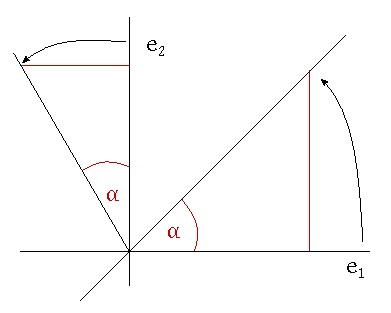
\includegraphics{img/13_rotation.pdf}
      \caption{Rotation in $\mathbb R^2$}
      \label{img:rotr2}
    \end{center}
  \end{figure}
\end{example}

\begin{example}[Rotation considered as motion]
  \begin{figure}[t]
    \begin{center}
      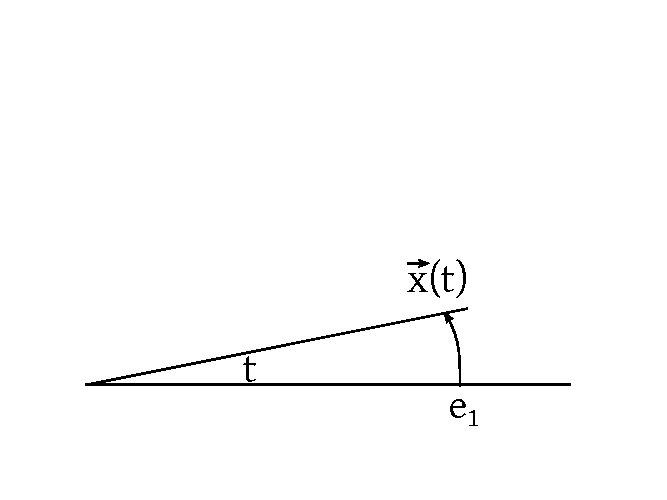
\includegraphics{img/14_rotation_as_motion.pdf}
      \caption{Rotation in $\mathbb R^2$ considered as motion. Commonly done by physicists.}
      \label{img:rotr2mot}
    \end{center}
  \end{figure}

  Tangent $a$:
  \[ \vectwo{x(t)}{y(t)} = \vectwo{\dot{x}(t)}{\dot{y}(t)} \]
  \[ \vec x(t) \bot \vec{x}(t) \]
  \[ \dot\vec{x}(t) = \begin{bmatrix} 0 & -1 \\ 1 & 0 \end{bmatrix} \vec{x}(t) \]
  \[ \vec{x}(t) = e^{\begin{bmatrix} 0 & -1 \\ 1 & 0 \end{bmatrix} t} \cdot \vec{x_0} \]
  Compare with Figure~\ref{img:rotr2mot}.

  \[ x'(t) = a\cdot x(t) \implies x(t) = c \cdot e^{at} \]
  \[ \frac{dx}{dt} = ax \]
  \[ dx = ax \cdot dt \]
  \[ \int \frac{dx}{x} = \int a \cdot dt \]
  \[ \log{x} = at + C \]
  \[ x = C_1 \cdot e^{at} \]

  \[ e^x = \sum_{n=0}^\infty \frac{x^n}{n!} \]
  \[ e^{\begin{bmatrix} 0 & -1 \\ 1 & 0 \end{bmatrix}t} = \sum_{n=0}^\infty \frac{\begin{bmatrix} 0 & -1 \\ 1 & 0 \end{bmatrix}^n}{n!} t^n \]
  \[ e^{it} = \cos{t} + i \cdot \sin{t} \]
  insert $\sum_{n=0}^\infty \frac{(it)^n}{n!}$ and split $\Re$ and $\Im$.

  \[ \begin{bmatrix} 0 & -1 \\ 1 & 0 \end{bmatrix}^2 = \begin{bmatrix} -1 & \\ & -1 \end{bmatrix} \]
  \[ \begin{bmatrix} 0 & -1 \\ 1 & 0 \end{bmatrix}^3 = \begin{bmatrix} 0 & -1 \\ 1 & 0 \end{bmatrix} \]
  \[ \begin{bmatrix} 0 & -1 \\ 1 & 0 \end{bmatrix}^4 = \begin{bmatrix} 1 &  \\  & 1 \end{bmatrix} \]

  \[ i^2 = -1 \qquad i^3 = -i \qquad i^4 = 1 \]

  \[
    e^{\begin{bmatrix} 0 & -1 \\ 1 & 0 \end{bmatrix} t} = \cos(t) \cdot \begin{bmatrix} 1 & \\ & 1 \end{bmatrix} + \sin(t) \cdot \begin{bmatrix} 0 & -1 \\ 1 & 0 \end{bmatrix} 
  \] \[
    U_{\alpha + \beta} = U_{\alpha} \cdot U_{\beta}
  \] \[
    \begin{bmatrix}
      \cos(\alpha + \beta) & -\sin(\alpha + \beta) \\
      \sin(\alpha + \beta) & \cos(\alpha + \beta)
    \end{bmatrix} =
    \begin{bmatrix}
      \cos\alpha & -\sin\alpha \\
      \sin\alpha & \cos\alpha
    \end{bmatrix} \cdot
    \begin{bmatrix}
      \cos\beta & -\sin\beta \\
      \sin\beta & \cos\alpha
    \end{bmatrix}
  \] \[
    =
    \begin{bmatrix}
      \cos\alpha \cos\beta - \sin\alpha \sin\beta & -\cos\alpha \cos\beta - \sin\alpha \sin\beta \\
      \sin\alpha \cos\beta + \cos\alpha \sin\beta & \sin\alpha \cos\beta + \cos\alpha \sin\beta
    \end{bmatrix}
  \]
\end{example}

\begin{example}[Reflection in $\mathbb R^2$]
  \[ S(e_1) = \begin{bmatrix} \cos(2\varphi) \\ \sin(2\varphi) \end{bmatrix} \]
  \[ S(e_2) = \begin{bmatrix} \cos(2\varphi - \frac\pi2) \\ \sin(2\varphi - \frac\pi2) \end{bmatrix} = \begin{bmatrix} \sin(2\varphi) \\ -\cos(2\varphi) \end{bmatrix} \]
  \[ \frac\pi2 - 2\psi = \frac\pi2 - 2(\frac\pi2 - \varphi) = 2\varphi - \frac\pi2 \]
  \[ S = \begin{bmatrix} \cos(2\varphi) & \sin(2\varphi) \\ \sin(2\varphi) & -\cos(2\varphi) \end{bmatrix} \]
\end{example}


\dateref{2018/05/07}

Linear isometries:

\begin{theorem} % 8.73
  \[ \mathcal O(n) = \setdef{U \in \mathbb R^{n\times n}}{U^TU = I} \qquad \text{ orthogonal group} \]
  \[ \mathcal U(n) = \setdef{U \in \mathbb C^{n\times n}}{U^*U = I} \qquad \text{ unitary group} \]
  \[ \mathcal{SO}(n) = \setdef{U \in \mathbb O}{\det(U) = 1} \subseteq \mathcal O(n) \qquad \text{ subgroup, special orthogonal group} \]
  \[ \mathcal{SU}(n) = \setdef{U \in \mathbb U}{\det(U) = 1} \subseteq \mathcal U(n) \qquad \text{ subgroup, special unitary group} \]
  \[ \mathcal{GL}(n, \mathbb K) = \setdef{A \in \mathbb K^{n\times n}}{\text{ invertible}} \qquad \text{ general linear group} \]
  \[ \mathcal{SL}(n, \mathbb K) = \setdef{A \in \mathbb \mathcal{GL}(n)}{\det(A) = 1} \qquad \text{ special linear group} \]
  Then, e.g. $\mathcal O(2)$ is the group of rotations and reflections.
\end{theorem}

\begin{remark}
  For $U \in \mathcal U(n)$ it holds that $\card{\det(U)} = 1$. Why?

  We know: $U^* U = I \implies \det(U^* U) = I = \det(U^*) \det(U) = \det(\overline{U}^T) \det(U) = \overline{\det(U^T)} \det(U) = \overline{\det(U)} \det(U) = \card{\det(U)}^2 = 1$.
\end{remark}

\begin{example}[Rotation]
  \[ U = \begin{bmatrix} \cos{\varphi} & -\sin{\varphi} \\ \sin{\varphi} & \cos{\varphi} \end{bmatrix} \]
  \[ \det{U_{\varphi}} = \cos^2(\varphi) + \sin^2(\varphi) = 1 \qquad \implies U_{\varphi} \in \mathcal {SO}(2) \]
  \[ S_{\varphi} = \begin{bmatrix} \cos(2\varphi) & \sin(2\varphi) \\ \sin(2\varphi) & -\cos(2\varphi) \end{bmatrix} \]
  \[ \det(S_{\varphi}) = -\cos^2(2\varphi) - \sin^2(2\varphi) = -1 \]

  General orthogonal matrix in $\mathcal O(2)$.
  \[ U = \begin{bmatrix} a & b \\ c & d \end{bmatrix} \text{ with } \overline U U = \begin{bmatrix} 1 & 0 \\ 0 & 1 \end{bmatrix} \]
  \[
    \begin{bmatrix} a & c \\ b & d \end{bmatrix} \begin{bmatrix} a & b \\ c & d \end{bmatrix}
    = \begin{bmatrix} a^2 + c^2 & ab + cd \\ ab + cd & b^2 + d^2 \end{bmatrix}
    \overset!= \begin{bmatrix} 1 & 0 \\ 0 & 1 \end{bmatrix}
  \]
  Resulting constraints:
  \begin{align}
    a^2 + c^2 &= 1 \\
    b^2 + d^2 &= 1 \\
    ab + cd &= 0 \\
  \end{align}
  \[ a = \cos\varphi \qquad c = \sin\varphi \qquad b = \cos\psi \qquad d = \sin\psi \]
  \[ \cos\varphi \cdot \cos\psi + \sin\varphi \cdot \sin\psi = 0 \]
  \[
    \begin{bmatrix} \cos\alpha & -\sin\alpha \\ \sin\alpha & \cos\alpha \end{bmatrix}
    \begin{bmatrix} \cos\beta & -\sin\beta \\ \sin\beta & \cos\beta \end{bmatrix}
    = \begin{bmatrix}
      \cos(\alpha + \beta) \\
    \end{bmatrix}
  \]
  \[ \cos \alpha \cos \beta - \sin \alpha \sin \beta = \cos(\alpha + \beta) \]
  \[ \cos \varphi \cdot \cos \psi = \cos(\varphi - \psi) \]
  \[ \cos \alpha = 0 \text{ for } \alpha = \frac\pi2 + k \cdot \pi = (k + \frac12) \pi \qquad (k \in \mathbb Z) \]
  \[ \implies \varphi - \psi = (k + \frac12) \pi \]
  \[ \varphi = \psi + (k + \frac12) \pi \]
  \begin{align*}
    \cos\varphi &= \cos(\psi + (k + \frac12) \pi) = \cos\psi \cos(k + \frac12) \pi - \sin\psi \underbrace{\sin(k + \frac12) \pi}_{\varepsilon \in \set{\pm 1}} \\
       &= -\varepsilon \cdot \sin\psi \implies \sin\psi = -\varepsilon \cos\varphi
  \end{align*}
  \[ \sin\alpha \cos\beta + \cos\alpha \sin\beta = \sin(\alpha + \beta) \]
  \[ \sin(\varphi) = \sin(\psi + (k + \frac12) \pi) = \underbrace{\sin\psi \cos\left(k + \frac12\right) \pi}_{= \varepsilon \cdot \cos(\psi)} + \underbrace{\cos \psi \sin \left(k + \frac12\right) \pi}_{= 0} \]
  \[ \cos\psi = \varepsilon \sin\varphi \]
  \[
    U = \begin{bmatrix} \cos\varphi & \varepsilon \cdot \sin(\psi) \\ \sin\varphi & -\varepsilon \cos\varphi \end{bmatrix}
    = \underbrace{\begin{bmatrix} \cos\varphi & -\sin\varphi \\ \sin\varphi & \cos\varphi \end{bmatrix}}_{\substack{\text{rotation} \\ \det = 1}} \cdot \underbrace{\begin{bmatrix} 1 & \\ & -\varepsilon \end{bmatrix}}_{\substack{\varepsilon = 1: \\ \text{reflection on x-axis} \\ \varepsilon = -1: \operatorname{id}}}
  \] \[
    U_{\varphi} = \cos\varphi \begin{bmatrix} 1 & \\ & 1 \end{bmatrix} + \sin\varphi \begin{bmatrix} & -1 \\ 1 & \end{bmatrix}
  \]
  Hence, every orthogonal matrix is either a rotation ($\det = 1$) or a reflection ($\det = -1$).

  \[ \mathcal{SO}(2): \set{U_{\varphi} = \cos\varphi + i \cdot \sin\varphi \qquad 1 = \begin{bmatrix} 1 & 0 \\ 0 & 1 \end{bmatrix}, i = \begin{bmatrix} 0 & -1 \\ 1 & 0 \end{bmatrix}} \]
  \[ \mathcal{SU}(2): \setdef{a_0 + i a_1 + j a_2 + k a_3}{\sum a_i^2 = 1} \]
\end{example}

\subsection{Quaternions}

William Rowan Hamilton (1805--1865).

\index{Quaternions}
\index{Complex numbers}
\begin{remark}[Quaternions]
  Hamilton defined the complex numbers in the modern sense in 1833.
  \[ \mathcal C = \setdef{(a,b)}{a,b \in \mathbb R} \]
  \[ (a,b) \cdot (c, d) = (ac - bd, ad + bc) \]
  He tried to invent them over 10 years for the third dimension.
  He failed.
  On 1843/10/16, he invented the quaternions next to a bridge.
  It works on four dimensions, but it is non-commutative.
  It is a screw field (\foreignlanguage{german}{Schiefk\"orper}).
  \[ ij = k \qquad jk = i \qquad ki = j \qquad ji = -k \qquad kj = -i \qquad ik = -j \]
  anti-commutative.
  \[ i^2 = j^2 = k^2 = -1 \]
  \[ (a_0 + a_1 i + a_2 j + a_3 k) (b_0 + b_1 i + b_2 j + b_3 k) \qquad \text{ linear} \]
  \[ (a_0 + \vec a) (b_0 + \vec b) = a_0 b_0 + a_0 \vec b + b_1 \vec a + \vec a \times \vec b \]
\end{remark}

\[ \mathcal{SO}(2) \eqsim \setdef{\cos\varphi + i \cdot \sin\varphi}{\varphi \in [0,2\pi]} = \setdef{z \in \mathbb C}{\card{z} = 1} = \mathcal T \text{ Torus} \]
\[ \mathcal{SU}(2) = \setdef{a_0 + i a_1 + j a_2 + k a_3}{\sum a_i^2 = 1} \]
\[ \mathcal{SO}(2) \eqsim \setdef{\cos \varphi + i \sin\varphi}{q \in [0,2\pi]} \]

\section{Polynomials and algebras}

\index{Algebra}
\begin{definition} % definition 9.1
  Let $\mathbb K$ be a field, a $\mathbb K$ algebra, a vector space $\mathcal A$ over $\mathbb K$
  with a multiplication operator $*: \mathcal A \times \mathcal A \to \mathcal A$ with $(a,b) \to a * b$ such that
  \begin{enumerate}
    \item $a * (b + c) = a * b + a * c$ (distributive law, $a, b, c \in \mathcal A$)
    \item $(a + b) * c = a * c + b * c$
    \item $\lambda \cdot (a * b) = (\lambda \cdot a) * b = a * (\lambda \cdot b)$ ($a, b \in \mathcal A, \lambda \in \mathbb K$, associativity)
  \end{enumerate}
\end{definition}

\index{Associative algebra}
\index{Commutative algebra}
\begin{remark} % Bemerkung 9.2
  \begin{description}
    \item[Associativity] is not generally required.
      \[ a * (b * c) = (a * b) * c \]
      If satisfied, it is called \emph{associative algebra}.
    \item[Commutativity] is not generally required.
      \[ a * b = b * a \]
      If satisfied, it is called \emph{commutative algebra}.
  \end{description}
\end{remark}

\index{Jacobian identity}
\index{Commutator}
\index{Lie algebra}
\index{Lie groups}
\index{Jordan algebra}
\begin{example} % Beispiel 9.3
  \begin{enumerate}
    \item $(\mathbb K, +, * = \cdot)$ is a one-dimensional $\mathbb K$ algebra.
    \item $(\mathbb K^{n \times n}, +, * = \text{ matrix multiplication})$ is an associative non-commutative algebra
      where $\mathbb K^{n \times n} \simeq \Hom(V, V)$ and $f * g = f \circ g$.
    \item $\mathbb K^\times = \set{f: X \to \mathbb K}$. Let $X$ be an arbitrary set.
      \[ (\lambda f + \mu g)(x) = \lambda \cdot f(x) + \mu \cdot g(x) \]
      \[ (f * g)(x) = f(x) \cdot g(x) \]
      $(\mathbb K^\times, +, *)$ is an associative, commutative algebra.
    \item $\mathbb R^3$ with $a \times b$ is an algebra.
      \[ a \times b = -b \times a \]
      is non-commutative and also non-associative:
      \[ a \times (b \times c) \neq (a \times b) \times c \]
      Jacobian identity:
      \[ a \times (b \times c) + b \times (c \times a) + c \times (a \times b) = 0 \]
    \item $\mathcal A = \mathbb K^{n\times n}$
      \[ A * B = [A,B] = A \cdot B - B \cdot A \qquad \text{\enquote{commutator}} \]
      is an algebra with Jacobian identity. Lie algebra:
      \[ [A, [B,C]] + [B, [C,A]] + [C, [A,B]] = 0 \]
      \[ [A,B] = -[B,A] \]
      The so-called Lie groups (like $\mathcal O(n), \mathcal U(n), \mathcal{SO}(n), \mathcal{SU}(n)$).
    \item
      $\mathcal A = \mathbb K^{n\times n}$
      \[ A * B = A \cdot B + B \cdot A \]
      is associative. It is an Jordan algebra.
      Pascual Jordan (1902--1980)\footnote{Different Jordan than in Gauss-Jordan and different than C. Jordan (19th century) about to come}.
  \end{enumerate}
\end{example}

O. Perron (1880/05/07--1975)

\index{Cauchy product}
\begin{definition} % Definition 9.4
  \[ \mathbb K^\infty = \setdef{(a_0, a_1, a_2, \dots)}{a_i \in \mathbb K} \]
  \[ P_{\mathbb K} = \setdef{(a_0, a_1, \dots, a_n, 0, \dots)}{n \in \mathbb N, a_i \in \mathbb K} \]
  Cauchy product:
  \[ (a_n)_{n \geq 0} * (b_n)_{n \geq 0} = (c_n)_{n \geq 0} \]
  \[ c_n = \sum_{k=0}^n a_k b_{n-k} \]
\end{definition}

\index{Polynomial algebra}
\index{Formal power series algebra}
\begin{lemma} % Lemma 9.5
  \begin{enumerate}
    \item $(P_{\mathbb K}, *)$ is a commutative, associative algebra with one-element $(1, 0, \dots)$.
      The basis is given with $1, x, x^2, \dots$. The algebra is called \emph{polynomial algebra}
      \[ \mathbb K[x] = \setdef{\sum_{k=0}^n a_k x^k}{a_k \in \mathbb K, n \in \mathbb N} \]
    \item $(\mathbb K^\infty, *)$ is a commutative algebra with one-element $(1, 0, \dots)$
      and is called \emph{algebra of formal power series}\footnote{We don't need to consider convergence. This is purely formal object.}
      \[ \mathbb K[[x]] = \setdef{\sum_{k=0}^\infty a_k x^k}{a_k \in \mathbb K} \]
  \end{enumerate}
\end{lemma}

\begin{proof}
  Show that $\forall a,b \in P_{\mathbb K}: a * b \in P_{\mathbb K}$, hence only finitely many $c_n$ are $\neq 0$.

  Remark: $a_k = 0 \forall k > m$ and $b_k = 0 \forall k > n$.

  \begin{claim}
    \[ c_k = 0 \forall k > m + n \]
  \end{claim}

  \begin{align*}
    c_k &= \sum_{l=0}^k a_l b_{k-l} \\
      &= \sum_{l=0}^{m-1} a_l b_{k-l} \qquad \text{equality if $l > m \implies a_l = 0$} \\
      &= 0
  \end{align*}
  \[ k > m + n, l < m \implies -l > -m \implies k - l \underbrace{>}_{\implies b_{k-l} = 0} m + n - m = n \]
  About the Cauchy product:
  \[ c_n = \sum_{k=0}^n a_k b_{n-k} = \sum_{k'=0}^n a_{n-k'} b_{k'} = (b * a)_n \qquad (k' = n - k) \]

  Law of distributivity:
  \begin{align*}
    [(a + b) * c]_n &= \sum_{k=0}^n (a + b)_k \cdot c_{n-k} \\
      &= \sum_{l=0}^n (a_k c_{n-k}) + (b_k c_{n-k}) \\
      &= (a * c)_n + (b * c)_n
  \end{align*}
\end{proof}

\index{Basis of a polynomial}
\index{Degree of a polynomial}
\begin{definition} % Definition 9.6
  Let $x^0 = (1, 0, \dots)$ and $x^k = (0, \dots, 1, 0, \dots)$ create a basis.
  The elements of $p(x) = \mathbb K[x]$ are called polynomials in the formal variable $x$
  \[ \deg{p(x)} = \max\setdef{k}{a_k \neq 0} \text{ is called \emph{degree of the polynomial}} \]
  \[ \deg(0) \coloneqq -\infty \]
\end{definition}

\begin{lemma}[Will be done in the practicals] % Lemma 9.7
  \begin{enumerate}
    \item $\deg(p(x) \cdot q(x)) = \deg(p(x)) + \deg(q(x))$
    \item $\mathbb K[x]$ is zero-divisor-free,
      hence $p(x) \cdot q(x) = 0 \implies p(x) = 0 \lor q(x) = 0$
  \end{enumerate}
\end{lemma}

\index{Polynomial function}
\begin{definition} % Definition 9.8
  Every polynomial $p(x) \in \mathbb K[x]$ induces a polynomial function $p: \mathbb K \to \mathbb K$ with $\alpha \mapsto p(\alpha)$
  with $p \in \mathbb K^{\mathbb K}$.
  \[ \implies (\lambda p + \mu q) (\alpha) = \lambda \cdot p(\alpha) + \mu \cdot q(\alpha) \]
  \[ (p \cdot q)(\alpha) = p(\alpha) \cdot q(\alpha) \]
  The map $\mathbb K[x] \to \mathbb K^{\mathbb K}$ with $p(x) \mapsto$ polynomial function $p$
  is linear and multiplicative (called \emph{algebra homomorphism}).
\end{definition}

\begin{remark} % Bemerkung 9.9
  A polynomial and a polynomial function are not the same.
  If $\card{\mathbb K} < \infty$, for example consider $\mathbb Z_5$.
  \[ \card{\mathbb Z_5^{\mathbb Z_5}} = 5^5 \]
  \[ \card{K[x]} = \infty \]
  For example, $\prod_{\alpha \in \mathbb K}(x - \alpha)$ corresponds to the polynomial function $0$.
  Hence the map $\mathbb K[x] \to \mathbb K^{\mathbb K}$ is surjective but not injective.

  On finite fields, every function is a polynomial function.
  \[ \eta_i = f(\xi_i) \qquad \set{\xi_1, \dots, \xi_n} = \mathbb K \]
  From the practicals, it will follow that there exists a polynomial of degree $n$ such that $p(\xi_i) = \eta_i$.
\end{remark}

\index{Algebra homomorphism}
\begin{definition} % Definition 9.10
  An algebra homomorphism is a linear map between $\psi$ and two $\mathbb K$-algebras $\mathcal A$ and $\mathcal B$ such that
  $\forall a,b \in \mathcal A: \psi(a * b) = \psi(a) * \psi(b)$.
\end{definition}

\begin{example} % Beispiel 9.11
  \begin{enumerate}
    \item $\mathbb K[x] \to \mathbb K^{\mathbb K}$ with $p(x) \mapsto$ polynomial function
    \item
      Let $\alpha \in \mathbb K$ be fixed.
      $\psi_{\alpha}: \mathbb K[x] \to \mathbb K$ with $p(x) \mapsto p(\alpha)$ is an algebra homomorphism of $\mathbb K[x] \to \mathbb K$.
      \[ \psi_\alpha(\lambda p + \mu q) = (\lambda p + \mu q)(\alpha) = \lambda p(\alpha) + \mu q(\alpha) = \lambda \psi_{\alpha}(p) + \mu \psi_{\alpha}(q) \]
    \item Consider $\iota: \mathbb K \to \mathbb K[x]$ with $\iota: \alpha \mapsto \alpha \cdot x^0$.
      \[ (\alpha \cdot x^0) \cdot (\beta \cdot x^0) = (\alpha \cdot \beta) \cdot x^0 \]
  \end{enumerate}
\end{example}

\begin{theorem}[Insertion theorem, dt. \foreignlanguage{german}{Einsetzungssatz}] % Satz 9.12
  Let $\mathcal A$ be an associative algebra with one-element $\mathbf 1_A$
  and $\iota: \mathbb K \to \mathcal A$ with $\alpha \mapsto \alpha \cdot \mathbf 1_A$ is the insertion of $\mathbb K$.

  Then for every $a \in \mathcal A$ the map
  \[ \psi_a: \mathbb K[x] \to \mathcal A \]
  \[ \sum_{k=0}^n c_k x^k \mapsto \sum_{k=0}^n c_k a^k \]
  of the unique algebra homomorphism of $\mathbb K[x] \to \mathcal A$ with the property $\psi_a(x) = a$.
  We say, $\mathbb K[x]$ is a \emph{free, associative algebra over $\mathbb K$}.
  Every algebra homomorphism $\mathbb K[x] \to \mathcal A$ has the structure.
\end{theorem}

\dateref{2018/05/09}

We consider algebras as vector spaces with associative multiplication. For example, matrices and polynomials.
An algebra homomorphism is linear and multiplicative.
\[ \Phi(a + b)= \Phi(a) * \Phi(b) \]
$A$ is an associative algebra with $\mathbf 1_A$.
\[ l: \substack{\mathbb K \to \mathcal A \\ \alpha \to \alpha \cdot \mathbf 1_{\mathcal A}} \]
$a \in \mathcal A \implies \mathcal L(a^0, a^1, a^2, a^3, \dots) \subseteq \mathcal A$ subalgebra.

\begin{enumerate}
  \item 
    \[ \exists! \Phi_a: \mathbb K[a] \to \mathcal A \text{ algebra homomorphism} \]
    such that $\Phi_a(x) = a$, namely $\Phi_a\left(\sum_{k=0}^n c_k x^k\right) = \sum_{k=0}^n c_k a^k$.
  \item
    Every homomorphism $\Psi: \mathbb K[x] \to \mathcal A$ has this structure.
    \begin{proof}
      Let $a = \Psi(x) \implies \Psi(x^n) = \Psi(x)^n = a^n$ by homomorphism.
      \[ \Psi \text{ linear } \implies \Psi\left(\sum_{k=0}^n c_k x^k\right) = \sum_{k=0}^n c_k \Psi(x^k) = \sum_{k=0}^n c_k a^k \]
      $x^0, x^1, \dots$ give a basis of $\mathbb K[x]$.
      Hence $\Psi = \Phi_a$ with $a = \Psi(x)$. On the opposite (1.): Obviously $\Phi_a$ is linear.
      Multiplicative: Show that
      \[ \underbrace{\Psi_a(p(x) \cdot q(x))}_{= p(a) \cdot q(a)} \overset!= \underbrace{\Phi_a(p(x)) \cdot {}_{\mathcal A}\Phi_a(q(x))}_{= p(a) \cdot q(a)} \]
    \end{proof}
\end{enumerate}

\begin{example} % Beispiel 9.13
  \begin{enumerate}
    \item $\mathcal A = \mathbb K$.
      \[ \Psi_\alpha: \substack{\mathbb K[x] \to \mathbb K \\ p(x) \mapsto p(\alpha)} \]
    \item $\mathcal A = \mathbb K^{n\times n} \eqsim \Hom(V, V)$
      \[ A^0 = I \qquad A^n = A \cdot A^{n-1} \]
      \[ l: \substack{\mathbb K \to \mathbb K^{n\times n} \\ \alpha \mapsto \alpha \cdot I} \]
      \[ \Psi_\alpha: \substack{\mathbb K[x] \to \mathbb K^{n\times n} \\ p(x) \mapsto p(A) \\ \sum_{k=0}^n c_k x^k \mapsto \sum_{k=0}^n c_k \cdot A^k}  \]
  \end{enumerate}
\end{example}

\begin{remark} % Bemerkung 9.14
  Let $\mathbb K[x]$ be a free, associative algebra over $\mathbb K$ with a generator.
  Hence, for all associative algebras $\mathcal A$, given some element $a \in \mathcal A$.
  There exists exactly one homomorphism $\varphi: \mathbb K[x] \to \mathcal A$ such that $\varphi(x) = a$.

  Compare it with a free group with one generator. Is a group $G$ generated by $x$ such that $\forall$ groups $H$, if $h \in H$ given,
  there exists exactly one group homomorphism $\varphi: G \to H$ such that $\varphi(x) = h$. Namely, $G = (\mathbb Z, +)$ is generated by $\mathbf 1$.
  Given $h \in H \to \varphi_h: \mathbb Z \to H_k$ and $k \mapsto h$.
\end{remark}

\index{Root of a polynomial}
\begin{definition}
  A \emph{root of a polynomial} $p(x) \in \mathbb K[x]$ is a $\xi \in \mathbb K$ such that $p(\xi) = \Psi_{\xi}(p) = 0$,
  hence $p(x) \in \ker{\Psi_{\xi}}$.
\end{definition}

\begin{remark}
  $p(x) = C_0$ is no root except $c_0 = 0$.

  $p(x) = c_0 + c_1 x$ is the only root, $\xi = -\frac{c_0}{c_1}$.

  \[ p(x) = c_0 + c_1 x + c_2 x^2 \]
  has two roots over $\mathbb C$.

  \[ p(x) = c_0 + c_1 x + c_2 x^2 + c_3 x^3 \]
  has three roots.

  To find roots, formulas up to fourth degree exist.
  For degree $\geq 5$, there is no equation.
\end{remark}

Paolo Ruffini (1765--1822) \\
Niels Henrik Abel (1802--1829) \\
Gerolamo Cardano (1501--1576)

\begin{remark}
  Cardano was a polymath.
  \begin{enumerate}
    \item founder of probability theory
    \item \emph{Liber de ludo aleae}: important book on probability
    \item Cardan joint (dt. \foreignlanguage{german}{Kardanische Welle})
    \item Gimbal (dt. \foreignlanguage{german}{Kardanische Aufh\"angung})
    \item used $\sqrt{-1}$ as a valid expression for the first time
    \item published a solution for roots of cubic polynomials (Ars Magna, 1545)
  \end{enumerate}

  Scipione del Ferro (1465--1526)

  \begin{enumerate}
    \item used a solution for roots of cubic polynomials in competitions, kept it secret
    \item came up with the same solution like Tartaglia
    \item lost competitions on cubic polynomials to Antonio Fiore, because Ferro's solution was not generic enough
  \end{enumerate}

  Niccol\`o Fontana Tartaglia (1500--1557)

  \begin{enumerate}
    \item Cardano cajoled Tartaglia into revealing his solution to the cubic equations by promising not to publish them.
  \end{enumerate}

  Ludovico Ferrari (1522--1565)
\end{remark}

\index{Method by Cardano/del Ferro}
\begin{theorem}[Method by Cardano/del Ferro] % 9.16
  \[ a_0 + a_1 x + a_2 x^2 + a_3 x^3 = 0 \]
  \[ x \to x + a \qquad \text{ such that } a_2 = 0 \]

  \[ x^3 + px + q = 0 \]
  Cubus p.6 rebus aeq 20 \\
  $x^3 + 6x = 20$

  $x = $ res, $x^2 = $ census, $x^3 = $ cubus.

  Approach: $x = u + v$.

  \[ u^3 + 3u^2v + 3uv^2 + v^3 + p(u + v) + q = 0 \]
  \[ u^3 + v^3 + (3uv + p)(u + v) + q = 0 \]

  Requirement:
  $u$ and $v$ such that $3uv + p = 0$.

  \[
    \begin{cases}
      u^3 + v^3 + q = 0 & \implies v^3 = -(q + u^3) \\
      3uv + p = 0 & \implies uv = -\frac{p}{3u}
    \end{cases}
  \]
  \[ u^3 \cdot v^3 = -\frac{p^3}{27} \]
  \[ -u^3 (q + u^3) = -\frac{p^3}{27} \]
  \[ u^6 + qu^3 - \frac{p^3}{27} = 0 \]
  \[ u^3 = ? \]

  Equation for degree 2 by Vi\`ete, Francois (1540--1603):

  \[ (y - \alpha)(x - \beta) = x^2 - (\alpha + \beta) x + \alpha \beta \]
  \[ x^2 + px + q \]
  \[ p = -(\alpha + \beta) \]
  \[ q = \alpha \cdot \beta \]

  \[ \alpha = \frac12 \left[(\alpha + \beta) + \sqrt{(\alpha - \beta)^2}\right] \]
  \[ \beta = \frac12 \left[(\alpha + \beta) - \sqrt{(\alpha - \beta)^2}\right] \]
  \[
    \frac\alpha\beta = \frac12 \left(\alpha + \beta \pm \sqrt{(\alpha - \beta)^2}\right)
    = \frac12 \left(\alpha + \beta \pm \sqrt{\underbrace{\alpha^2 + \beta^2 - 2\alpha\beta}_{(\alpha + \beta)^2 - 4\alpha\beta}}\right)
    = \frac12 \left(-p \pm \sqrt{p^2 - 4q}\right)
  \]

  Hence,
  \begin{align*}
    u^3 &= \frac12\left(-q \mp \sqrt{q^2 + \frac{4p^3}{27}}\right) \\
    u^3 &= \frac{q}2 \pm \sqrt{\frac{q^2}{4} + \frac{p^3}{27}} \\
    u &= \sqrt[3]{-\frac{q}2 \pm \sqrt{\frac{q^2}{4} + \frac{p^3}{27}}} \\
    v^3 &= -q - u^3 = -\frac{q}{2} \mp \sqrt{\frac{q^2}{4} + \frac{p^3}{27}} \\
    x = u + v &= \sqrt[3]{-\frac{q}2 + \sqrt{\frac{q^2}{4} + \frac{p^3}{27}}} + \sqrt[3]{-\frac{q^2}{2} - \sqrt{\frac{q^2}{4} + \frac{p^3}{27}}}
  \end{align*}
\end{theorem}

\index{Polynomial division}
\begin{theorem}[Division with remainder] % 9.17 Satz
  $p(x), q(x) \in \mathbb K[x]$, $q(x) \neq 0$.

  Then there exists exactly one polynomial $s(x), r(x) \in \mathbb K[x]$,
  \[ p(x) = s(x) \cdot q(x) + r(x) \]
  with $\deg{r(x)} < \deg{q(x)}$.
\end{theorem}

\begin{proof}
  Induction over $\deg{p(x)}$.
  \begin{description}
    \item[Induction base]
      \[ \deg{p(x)} < \deg{q(x)} \leadsto p(x) = 0 \cdot q(x) + p(x) \]
      If $\deg{p(x)} \geq \deg{q(x)}$,
      \[ p(x) = \sum_{k=0}^n a_k x^k \qquad q(x) = \sum_{k=0}^m b_k x^k  \]
      \[ a_n \neq 0 \qquad m \leq n \qquad b_m \neq 0 \]

      \begin{align*}
        p_1(x) &= p(x) - \frac{a_n}{b_m} \cdot q(x) \cdot x^{n-m} \
      \intertext{cancels the largest term $a_n x^n$ in $p(x)$.}
          &= \sum_{k=0}^n a_k x^k - \frac{a_n}{a_m} \sum_{k=0}^m b_k x^{k+n-m} \\
          &= a_n x^n + \sum_{k=0}^{n-1} a_k x^k - \frac{a_n}{a_m} b_m \cdot x^{m+n-m} - \frac{a_n}{b_m} \sum_{k=0}^{m-1} b_k x^{k+n-m} \\
      \end{align*}
      what remains is a polynomial of degree $\deg{p_1(x)} \leq n-1$.
      \[ \implies p(x) = \frac{a_n}{b_m} x^{n-m} \cdot q(x) + p_1(x) \]
      By induction hypothesis,
      \[ p_1(x) = s_1(x) \cdot q(x) + r_1(x) \]
      Hence,
      \[ p(x) = \left(\frac{a_n}{a_m} x^{n-m} + s_1(x)\right) q(x) + r_1(x) \]
  \end{description}
\end{proof}

\begin{example} % Beispiel 9.18
  \begin{align*}
    p(x) &= 3x^5 - x^4 + 2x^3 + x^2 + 1 \\
    q(x) &= x^2 - 3x + 1 \\
  \end{align*}
  \[
    \begin{vmatrix}
      3x^5 &- x^4 &+ 2x^3 &+ x^2 &+ 1 &: x^2 &- 3x &+ 1 &= 3x^2 + 8x^2 + 23x + 62 \\
      -3x^5 & +9x^4 & -3x^3 \\
      0 & 8x^4 & -x^3 & +x^2 & +1 \\
        & 8x^4 & -24x^3 & +8x^2 \\
        & 0 & 23x^3 & -7x^2 & +1 \\
        &   & 23x^3 & -69x^2 & +23x \\
        &   & 0     & 62x^2 & -23x & +1 \\
        &   &       & 62x^2 & -186x & +62 \\
        &   &       &       & 163x & -61
    \end{vmatrix}
  \]
  Hence, $s(x) = 3x^3 + 8x^2 + 23x + 62$ and $r(x) = 163x - 61$.
\end{example}

\begin{definition} % 9.19
  $q(x)$ \emph{divides} $p(x)$ is the remainder is zero.

  There exists $s(x)$ such that $p(x) = s(x) \cdot q(x)$.
\end{definition}

\begin{theorem} % Satz 9.20
  \begin{enumerate}
    \item If $p(x) = s(x) \cdot (x - \xi) + r$
      \[ q(x) = x - \xi \qquad \implies p(\xi) = r \]
    \item $\xi$ is root of $p(x) \implies x - \xi$ divides $p(x)$
  \end{enumerate}
\end{theorem}

\begin{theorem}[Ruffini-Horner's method]
  Given $p(x) \in \mathbb K[x]$, $\lambda \in \mathbb K$. \\
  Find $p(\lambda)$.

  \begin{align*}
    p(x) &= a_n x^n + a_{n-1} x^{n-1} + \dots + a_1 x + a_0 \\
      &= a_n \lambda^n + a_{n-1} \lambda^{n-1} + \ldots + a_1 \lambda + a_0 \\
      &= \left(a_n \lambda^{n-1} + \dots + a_n\right) \lambda + a_0 \\
      &= \left((a_n \lambda^{n-2} + \dots + a_n) \lambda + a_1\right) \lambda + a_0 \\
      &= \vdots
  \end{align*}

  Algorithm:
  \[ \xi_n = a_n \text{ for } k = n-1, \dots, 0 \qquad \xi_k = \lambda \xi_{k+1} + a_k \]
  \[ p(\lambda) = \xi_0 \]
  If $p(x) = s(x) (x - \lambda) + r$, $p(\lambda) = r$.
\end{theorem}

\begin{example} % Beispiel 9.22
  \[ 3x^5 - x^4 + 2x^3 + x^2 + 1 \]
  \[ p(5) = ? \qquad \xi_5 = 3 \]
  \[
    \begin{vmatrix}
      3x^5 & -x^4 & +2x^3 & +x^2 & +1 & : (x - 5) & = & 3x^4 + 14x^3 + 72x^2 + 361x + 1805 \\
      3x^5 & -15x^4 \\
      0    & 14x^4 & +2x^3 & +x^2 & +1 \\
           & 14x^4 & -70x^3 & \\
           & 0     & +72x^3 & +x^2 & +1 \\
           &       & 72x^3 & -360x^2 \\
           &       & 0     & +361x^2 & +1 \\
           &       &       & 361x^2 & -1805x \\
           &       &       &        & 1805x & +1 \\
           &       &       &        & 1805x & -5 \cdot 1805 \\
           &       &       &        &       & 5 \cdot 1805+1
    \end{vmatrix}
  \]
  \[ \xi_5 = 3 \]
  \[ \xi_4 = 5 \cdot \xi_5 + (-1) = 5 \cdot 3 - 1 = 14 \]
  \[ \xi_3 = 5 \cdot 14 + 2 = 72 \]
  \[ \xi_2 = 5 \cdot 72 + 1 = 361 \]
  \[ \xi_1 = 5 \cdot 361 + 0 = 1805 \]
  \[ \xi_0 = 5 \cdot 1805 + 1 = 9026 \]
\end{example}

\index{Reducible polynomial}
\index{Irreducible polynomial}
\index{Factorization of a polynomial}
\begin{definition} % 9.23
  A polynomial $p(x) \in \mathbb K[x]$ is called \emph{reducible},
  if $\exists p_1(x), p_2(x): \deg{p_1(x)} < \deg{p(x)}$ and $p(x) = p_1(x) \cdot p_2(x)$ (is the factorization).
  $\deg{p_2(x)} < \deg{p(x)}$ (proper divisor).
  Otherwise the polynomial is called \emph{irreducible}.
\end{definition}

\begin{remark} % Bemerkung 9.24
  An irreducible polynomial of degree $>1$ has no roots.
\end{remark}

\begin{example} % Beispiel 9.25
  \begin{itemize}
    \item
      Consider $x^2 = -2$ irreducible over $\mathbb Q \subseteq \mathbb R \subseteq \mathbb R$.
      Its roots are $\pm \sqrt2$.

      It is reducible over $\mathbb R$: $x^2 - 2 = (x - \sqrt2)(x + \sqrt2)$. \\
      It is reducible over $\mathbb Q(\sqrt{2}) = \setdef{a + b\sqrt{2}}{a,b \in \mathbb Q}$.
    \item
      Consider $x^2+1$ irreducible over $\mathbb Q, \mathbb R$ and reducible over $\mathbb C$.
      Its roots are $\pm i$.

      $\mathbb Q(i) = \setdef{a + bi}{a,b \in \mathbb Q}$.
      $x^2 + 1 = (x + i)(x - i)$.
    \item
      Consider $\mathbb K = \mathbb Z_2$ and $p(x) = x^2 + x + 1$.
      This polynomial has no roots and is irreducible.
    \item
      $x^5 + x + 1$ has no roots, is reducible.
      \[ x^5 + x + 1 = (x^2 + x + 1)(x^3 + x^2 + 1) \]
      Is there some field $\mathbb K \supseteq \mathbb Z_2$ such that $x^3 + x^2 + 1$ has roots?

      \underline{Yes}. Let $\alpha$ be a number such that $\alpha^3 + \alpha^2 + 1 = 0 \implies \alpha^3 = -\alpha^2 - 1 = \alpha^2 + 1$.
      \[ \mathbb K = \mathbb Z_2(\alpha) = \setdef{a + b\alpha + c\alpha^2}{a,b,c \in \mathbb Z_2} \]
      with $\alpha^3 = \alpha^2 + 1$ is a field.

      Let $i$ be a number such that $i^2 + 1 = 0$, thus $i^2 = -1$
      \[ \mathbb C = \mathbb R(i) = \setdef{a + bi}{a,b \in \mathbb R} \]
  \end{itemize}
  Hence, irreducible is not equivalent to some root exists.
  The implication works only in one direction.
  There always exists some field such that roots exist.
\end{example}

\begin{theorem}[Fundamental theorem of Algebra] % Satz 9.26
  $\mathbb C$ is algebraically closed, hence every polynomial has a root over $\mathbb C$.
\end{theorem}

\begin{corollary}
  Every polynomial over $\mathbb C$ \dots
  \begin{enumerate}
    \item has a factorization $p(x) = (x - \xi_1) (x - \xi_2) \dots (x - \xi_n)$.
    \item $p(x)$ is irreducible $\iff \deg{p(x)} \leq 1$.
  \end{enumerate}
\end{corollary}
\begin{remark}
  No algebraic proof exists. It is more like a Fundamental Theorem of Calculus over complex numbers.
  The proof is given by the Lionville theorem (not done here).
\end{remark}

\begin{theorem} % Satz 9.27
  For arbitrary fields, it holds that
  every polynomial has exactly one factorization (except for its order) in irreducible factors.
\end{theorem}

\dateref{2018/05/14}

\subsection{The greatest common divisor of polynomials}

The Euclidean algorithm determines the greatest common divisor.

Consider $n = q \cdot m + r$. For the Euclidean algorithm, it holds that $\operatorname{gcd}(n, m) = \operatorname{gcd}(m, r)$
The analogous solution holds for polynomials. Consider $p(x) = s(x) \cdot q(x) + r(x)$.
Then the $\operatorname{gcd}(p(x), q(x))$ returns the polynomial of maximum degree that divides the polynomial with leading coefficient $1$.

\begin{corollary}
  The Euclidean algorithm also works for polynomials.
\end{corollary}

An application: Find all multiple roots (i.e. roots with multiplicity greater 1).
\[ (x - \xi)^k | p(x) \]
\[ \implies (x - \xi)^{k-1} | p'(x) \]

\[ p(x) = s(x) \cdot (x - \xi)^k \]
\[ p'(x) = s'(x) \cdot (x - \xi)^k + s(x) \cdot k \cdot (x - \xi)^{k-1} = (s'(x) (x - \xi) + s(x) \cdot k) (x - \xi)^{k-1} \]
\[ \implies (x - \xi)^{k-1} | \operatorname{gcd}(p(x), p'(x)) \]

\section{Eigenvectors and eigenvalues}

Given $f: V \to V$. Find a basis of $V$ such that $\Phi_B^B(f)$ has the simplest possible representation.
Hence,
\[ A = \Phi_B^B(f) = \begin{bmatrix} a_{11} &  & 0 \\ & \ddots & \\ 0 &  & a_{nn} \end{bmatrix} \]
\[ A \cdot e_i = \lambda_i \cdot e_i \]
Find vector $v \in V$ such that $f(v) = \lambda \cdot v$.

\begin{figure}[t]
  \begin{center}
    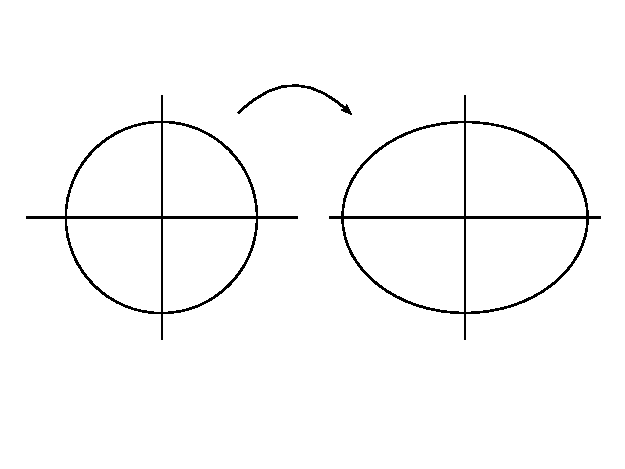
\includegraphics{img/15_screwing_map.pdf}
    \caption{How map $f$ transforms a circle}
  \end{center}
\end{figure}

\index{Eigenvalue}
\index{Eigenvector}
\index{Spectrum}
\begin{definition} % Definition 10.1
  $f \in \operatorname{Hom}(V, V) = \operatorname{End}(V)$.
  $\lambda \in \mathbb K$ is called \emph{eigenvalue} if
  $\exists v \in V \setminus \set{0}: f(v) = \lambda \cdot v$.
  Then $v$ is called \emph{eigenvector} of eigenvalue $\lambda$.
  $\operatorname{spec}(f) = \set{\text{eigenvalues of } f}$ is called \emph{spectrum of $f$}.
\end{definition}

In 1925 in quantum mechanisms, it was discovered that the spectrum of light is given as a linear map (spectrum in the mathematical sense).

\index{Eigenspace}
\begin{lemma}
  For $\lambda \in \mathbb K$, $f \in \operatorname{End}(V)$.
  \[ \eta_{\lambda} = \set{v}{f(v) = \lambda \cdot v} \]
  is a subspace and is called eigenspace of $f$ for eigenvalue $\lambda$.
\end{lemma}
\begin{proof}
  \begin{align*}
    f(v) = \lambda \cdot v \iff f(v) - \lambda \cdot v &= 0 \\
    (f - \lambda \cdot \operatorname{id}) (v) &= 0 \\
    \iff v \in \underbrace{\operatorname{ker}(f - \lambda \cdot \operatorname{id})}_{\text{subspace}} &
  \end{align*}
\end{proof}

\begin{example} % Beispiel 10.3
  \begin{enumerate}
    \item $f = \mu \cdot \operatorname{id}$. $\operatorname{spec}(f) = \set{\mu}$. $f(v) = \mu \cdot v \forall v \in V$. $\eta_\mu = V$.
    \item Let $b_1, \dots, b_n$ be a basis of $V$. Let $\lambda_1, \dots, \lambda_n \in \mathbb K$.
      Then there exists a unique, linear map $f$ such that $f(b_i) = \lambda_i \cdot b_i$.
      Every $b_i$ is an eigenvector to eigenvalue $\lambda_i$.
      \[ \eta_{\lambda} = \mathcal L(\setdef{b_i}{\lambda_i = \lambda}) \]
      Assume $f(v) = \lambda \cdot v$.
      \begin{align*}
        v &= \alpha_1 \cdot b_1 + \dots + \alpha_n b_n \\
        f(v) &= \alpha_1 f(b_1) + \dots + \alpha_n f(b_n) \\
          &= \alpha_1 \lambda_1 b_1 + \dots + \alpha_n \lambda_n b_n \\
          &= \lambda(\alpha_1 b_1 + \dots + \alpha_n b_n) \\
        \hline
        \implies 0 &= \alpha_1(\lambda_1 - \lambda) b_1 + \dots + \alpha_n(\lambda_n - \lambda) \cdot b_n \\
        \text{linear indep.} \implies& \forall i: \alpha_i (\lambda_i - \lambda) = 0 \\
        \text{hence either } \alpha_i = 0 \text{ or } \lambda_i = \lambda
      \end{align*}
      \[ \implies \operatorname{spec}(f) = \set{\lambda_1, \dots, \lambda_n} \]
      \[ \Phi_B^B(f) = \begin{bmatrix} \lambda_1 & & 0 \\ & \ddots & \\ 0 & & \lambda_n \end{bmatrix} \]
    \item Let $V = C^{\infty}(\mathbb R)$.
      \[ \frac{d}{dx} y(x) = \lambda \cdot y(x) \qquad \frac{dy}{dx} = \lambda \cdot y \]
      \[ \int \frac{dy}{y} = \int \lambda \cdot dx \]
      \index{Eigen function}
      \[ \operatorname{log}(y) = \lambda \cdot x + C \qquad \text{ \emph{Eigen function} (compare with Fourier analysis)} \]
      \[ y = C \cdot e^{\lambda x} \]
      \[ \frac{d}{dx} e^{\lambda x} = \lambda \cdot e^{\lambda x} \]
    \item Let $V = C^{\infty}[0, a]$.
      \begin{align*}
        \frac{d^2}{dx^2} y(x) &= \lambda \cdot y(x) \\
        \frac{d^2}{dx^2} e^{\lambda x} &= \frac{d}{dx} \lambda e^{\lambda x} = \lambda^2 e^{\lambda x} \\
        \frac{d^2}{dx^2} e^{i \omega x} &= -\omega^2 e^{i\omega x} \\
        \frac{d^2}{dx^2} \sin{\omega x} &= \frac{d}{dx} \omega \cdot \cos(\omega x) = -\omega^2 \cdot \sin(\omega x) \\
        \frac{d^2}{dx^2} \cos{\omega \alpha} &= \frac{d}{dx} (-\omega) \sin(\omega x) = -\omega^2 \cos(\omega x)
      \end{align*}
      \[ y(0) = y_0 \to y(x) = y_0 \cdot e^{\lambda x} \]
      \[ y(0) = y(a) = 0 \]
      \[ y(x) = \sin(\omega x) \]
      \[ \omega a = k \cdot \pi \implies y(0) = y(a) = \pi \]
      \[ \omega = \frac{k \cdot \pi}{a} \]
      Eigen values of $H = P^2 + Q$ and $PQ - QP = \frac{\hbar}{i} I$. Heisenberg: Quantum mechanics is not commutative (impulses are matrices, not values).
  \end{enumerate}
\end{example}

\index{Right-sided eigenvalue}
\index{Left-sided eigenvalue}
\begin{definition} % Definition 10.4
  Let $A$ be a $n \times n$ matrix.
  $\lambda$ is called right-sided eigenvalue if $\exists x \in \mathbb K^n \setminus \set{0}: Ax = \lambda \cdot x$.
  $\lambda$ is called left-sided eigenvalue if $\exists x \in \mathbb K^n \setminus \set{0}: x^T A = \lambda \cdot x^T$
  But this definition is satisfied $\iff A^T x = \lambda \cdot x$, hence right-sided eigenvalue of $A^T$.
  Thus, these definitions collapse.
\end{definition}

\begin{lemma} % Lemma 10.5
  Left-sided eigenvalue $\iff$ right-sided eigenvalue.
  Let $\lambda$ be a right-sided eigenvalue.
  \begin{align*}
    Ax = \lambda x &\iff (A - \lambda \cdot I) \cdot x = 0 \\
      &\iff \exists x \neq 0: x \in \ker(A - \lambda I) \\
      &\iff \ker(A - \lambda I) \neq \set{0} \\
      &\iff \rank(A - \lambda I) < n \\
      &\iff \rank(A^T - \lambda I) < n \\
      &\iff \ker(A^T - \lambda I) \neq \set{0} \\
      &\iff \exists x \neq 0: A^T x = \lambda \cdot x \\
      &\iff \lambda \text{ is a left-sided } eigenvalue
  \end{align*}
\end{lemma}

\begin{example} % Beispiel 10.6
  For $\dim = \infty$, this must not hold.
  \[ S: \substack{\mathbb K^\infty \to \mathbb K^\infty \\ (x_1, x_2, \dots) \mapsto (x_2, x_3, \dots)} \]
  \[ S(1, 0, \dots) = (0, 0, \dots) \]
  \[ \implies (1, 0, \dots) \text{ is eigenvector for eigenvalue } 0 \]
  hence, element of $\ker(S)$.
  \[
    S = \begin{bmatrix}
      0 & 1 & 0 & 0 \\
      \vdots & 0 & 1 & 0 \\
      \vdots & \vdots & 0 & 1 \\
      \vdots & \vdots & \vdots & 0 \\
      \vdots & \vdots & \vdots & \vdots \\
      0 & & &
    \end{bmatrix}
  \] \[
    S^T = \begin{bmatrix}
      0 & & & \\
      1 & 0 &  & 0 \\
        & 1 & \ddots & \\
        & \ddots & \ddots & \\
      0 &  & 1 & 0
    \end{bmatrix}
  \]
  $S^T(x_1, x_2, \dots) \mapsto (0, x_1, x_2)$ is injective.
  $\ker(S^T) = \set{0}$. Hence $0$ is no eigenvalue.
  $0$ is right-sided eigenvalue of $S$, but not left-sided eigenvalue.
\end{example}

\begin{remark}
  The theory of eigenvalues in infinite-dimensional spaces is more complex then the finite-dimensional case.
\end{remark}

\begin{definition} % Definition 10.7
  For $A \in \mathbb K^{n \times n}$.
  \begin{align*}
    \operatorname{spec}(A) &= \set{\text{right-sided eigenvalue of } A} \\
        &= \set{\text{left-sided eigenvalue of } A}
  \end{align*}
  is called \emph{spectrum of $A$}.
\end{definition}

\begin{remark}[Proof exercise]
  $\dim{V} = n, f \in \operatorname{End}(V), B$ is basis of $V$.
  \[ \implies \operatorname{spec}(f) = \operatorname{spec}(\Phi_B^B(f)) \]
\end{remark}

\begin{corollary}
  The spectrum does not depend on the choice of the basis. Hence,
  \[ \operatorname{spec}(T^{-1} AT) = \operatorname{spec}(A) \]

  \begin{proof}[Direct proof]
    \begin{align*}
      Ax &= \lambda x \\
      A \cdot T \cdot T^{-1} x &= \lambda \cdot x \\
      \implies T^{-1} AT \cdot T^{-1} x &= \lambda T^{-1} x \\
        &\text{ if } x \text{ is eigenvector of } A \\
      \implies y = T^{-1} x &\text{ eigenvector of } T^{-1} AT
    \end{align*}
  \end{proof}
\end{corollary}

\begin{remark}
  $\lambda$ is eigen value of $A$.
  \begin{align*}
    &\iff \ker(\lambda \cdot I - A) \neq \set{0} \\
    &\iff \rank(\lambda \cdot I - A) < n \\
    &\iff \det(\lambda \cdot I - A) = 0
  \end{align*}
\end{remark}

\index{Characteristic polynomial}
\begin{theorem}[Theorem and definition] \hfill{} % Satz & Definition 10.10
  \begin{enumerate}
    \item $\chi_A(\lambda) \coloneqq \det(\lambda \cdot I - A)$ is a polynomial function and is called \emph{characteristic polynomial of $A$}.
    \item $\lambda$ is eigenvector $\iff \chi_A(\lambda) = 0$
  \end{enumerate}
\end{theorem}

\begin{example} % Beispiel 10.11
  \[
    A = \begin{bmatrix}
      -1 & 1 & 2 \\
      -1 & -5 & 2 \\
      2 & -2 & -4
    \end{bmatrix}
  \]
  \[
    \chi_A(\lambda) = \det(\lambda I - A)
    = \begin{vmatrix}
      \lambda + 1 & -1 & -2 \\
      1 & \lambda + 5 & -2 \\
      -2 & 2 & \lambda+4
    \end{vmatrix}
    = \begin{vmatrix}
      \lambda+1 & -1 & -2 \\
      1 & \lambda+5 & -2 \\
      0 & 2\lambda+12 & \lambda
    \end{vmatrix}
  \] \[
    = \begin{vmatrix}
      \lambda & -\lambda-6 & 0 \\
      1 & \lambda+5 & -2 \\
      0 & 2\lambda+12 & \lambda
    \end{vmatrix} = \lambda \cdot \begin{vmatrix}
      \lambda+5 & -2 \\
      2\lambda+12 & \lambda
    \end{vmatrix}
    - \begin{vmatrix}
      -\lambda - 6 & 0 \\
      2\lambda+12 & \lambda
    \end{vmatrix}
  \] \[
    = \lambda \cdot [\lambda^2 + 5\lambda + 4\lambda + 24] - \lambda(-\lambda-6)
  \] \[
    = \lambda(\lambda^2 + 5\lambda + 4\lambda + 24 + \lambda + 6)
  \] \[
    = \lambda(\lambda^2 + 10\lambda + 30)
  \] \[
    x_1 = 0 \qquad \lambda_{2,3} = \frac{-10 \pm \sqrt{10^2 - 120}}{2} = \frac{-10 \pm 2\sqrt{-5}}{2} = -5 \pm i\sqrt{5}
  \]
  Thus, the existence of eigenvalues depends on the field.
\end{example}

\index{Symmetrical minors}
\begin{theorem} % Satz 10.12
  Let $A \in \mathbb K^{n \times n}$.
  \[ \implies \chi_A(x) = \det(x \cdot I - A) \text{ is polynomial of degree } n \]
  specifically, $\chi_A(x) = \sum_{k=0}^n (-1)^{n-k} c_k(A) \cdot x^k$ with $c_k(A) = \sum_{\substack{j \in \set{1, \dots, n} \\ |j| = n - k}} \det(A_{jj})$
  with $A_{jj} = (a_{ij})_{\substack{i \in J \\ j \in J}}$ called \emph{symmetrical minors}.

  What are values of $c_i$?
  \begin{align*}
    c_0 &= \det(A) \\
    C_n &= 1 \\
    C_{n-1} &= \sum a_{ii} = \operatorname{Tr}(A)
  \end{align*}
\end{theorem}

\begin{proof}
  The proof is given using the Leibniz formula for determinants.

  \begin{align*}
    \det(x \cdot I - A) &= \sum_{\pi \in \sigma_n} (-1)^\pi \prod_{i=1}^n \underbrace{(x \cdot I - A)_{\pi(i),i}}_{x \cdot \delta_{\pi(i),i} - a_{\pi(i),i}} \\
      &= (x - a_{11})(x - a_{22}) \dots (x - a_{nn}) +
        \underbrace{
          \sum_{\substack{\pi \in \sigma_n \\ \pi \neq \operatorname{id}}}
          (-1)^\pi \prod_{i=1}^n
          \left(x \delta_{\pi(i),i} - a_{\pi(i),i}\right)
        }_{\text{for at least 2 $i$, $\delta_{\pi(i),i} = 0$}} \\
      &= \text{ expression of degree } n + \text{ expression of degree } n -2
  \end{align*}
  Hence $x^n$ stays the same. Hence the degree of $\chi_A(x)$ is $n$.
  \begin{align*}
    \det{\prod_{i=1}^n (x \delta_{\pi(i),i} - a_{\pi(i),i})} &= \#\setdef{i}{\pi(i) = i} \\
      &= \#\operatorname{fixedpoints}(\pi)
  \end{align*}
  Let $s_1, \dots, s_n$ be the columns of $A$.
  \[ \det(xI - A_i) = \triangle(x\cdot e_1 - s_1, x \cdot e_2 - s_2, \dots, x \cdot e_n - s_n) = \sum_{I \subseteq \set{1, \dots, n}} \triangle(y_1, \dots, y_n) \]

  \[ y_i = \begin{cases} x \cdot e_i & i \in I \\ -s_{i_k} & i \in I^C \end{cases} \]
  Let $k \in I$.
  \[
    \triangle(y_1, \dots, y_{k-1}, x \cdot e_k, y_{k+1}, \dots, y_n) = \begin{vmatrix}
      y_1 & y_2 & \dots & y_{k-1} & 0 & y_{k+1} & \dots & y_n \\
      \vdots & \vdots & \vdots & \vdots & \vdots & \vdots & \vdots & \vdots \\
      \vdots & \vdots & \vdots & \vdots & 0 & \vdots & \vdots & \vdots \\
      \vdots & \vdots & \vdots & \vdots & x & \vdots & \vdots & \vdots \\
      \vdots & \vdots & \vdots & \vdots & 0 & \vdots & \vdots & \vdots \\
      \vdots & \vdots & \vdots & \vdots & \vdots & \vdots & \vdots & \vdots \\
      \vdots & \vdots & \vdots & \vdots & 0 & \vdots & \vdots & \vdots
    \end{vmatrix}
  \]
  Permute the $k$-th column into the first column: $(-1)^{k-1}$. \\
  Permute the $k$-th row into the first row: $(-1)^{k-1}$.
  \[
    = \begin{vmatrix}
      x & \tilde{y_1} & \tilde{y_2} & \dots & \tilde{k-1} & \tilde{k+1} & \dots & \tilde{n} \\
      0 & \vdots & \vdots & \vdots & \vdots & \vdots & \vdots & \vdots \\
      \vdots & \vdots & \vdots & \vdots & \vdots & \vdots & \vdots & \vdots \\
      0 & \vdots & \vdots & \vdots & \vdots & \vdots & \vdots & \vdots \\
    \end{vmatrix}
    = x \cdot \begin{vmatrix}
      \tilde{\tilde{y_1}} & \dots & \tilde{\tilde{y_{k-1}}} & \tilde{\tilde{y_{k+1}}} & \vdots & \tilde{\tilde{y_n}} \\
      \vdots & \vdots & \vdots & \vdots & \vdots & \vdots
    \end{vmatrix}
  \]
  where $\tilde{y}$ is the permutation of $y_i$ such that the $k$-th row moved to the first.

  Every time, one $x$ is eliminated, the corresponding row and column of $A$ is removed.
  In the end,
  \[ x^{\card{I}} \cdot \underbrace{\det{A_{I^C I^C}}}_{\text{minor of the complement $\card{I^C} = n-k$}} \cdot (-1)^{\card{I^C}} \]
  \begin{align*}
    \implies \chi_A(x) &= \sum_{I \subseteq \set{1, \dots, n}} x^{\card{I}} \cdot \det[A_{I^C I^C}] (-1)^{\card{I^C}}
      &= \sum_{k=0}^n x^k (-1)^{n-k} c_k(A)
  \end{align*}
  with $c_k(A) = \sum_{\card{J} = n-k} \det[A_{jj}]$.
\end{proof}

\dateref{2018/05/16}

\[ Ax = \lambda x \]
\[ x \in \ker(\lambda \cdot I - A) \]
\[ \chi_A(\lambda) = \det(\lambda I - A) = x^n - \operatorname{Tr}(A) x^{n-1} + \dots (-1)^n \det(A) \]
Characteristic polynomial: $= \sum_{k=0}^n (-1)^{n-k} c_k x^k$
\[ c_k = \sum_{\card{J} = n-k} \det[A_{J,J}] \]
\[ T^{-1} AT \cdot T^{-1} x = \lambda T^{-1} x \]

\begin{lemma} % 10.13
  \[ \chi_{T^{-1} AT}(x) = \chi_A(x) \]
\end{lemma}
\begin{proof}
  \begin{align*}
    \chi_{T^{-1}AT}(x) &= \det(xI - T^{-1}AT) \\
      &= \det(x T^{-1} T - T^{-1} AT) \\
      &= \det(T^{-1}(xI - A) \cdot T) \\
      &= \det(T^{-1}) \cdot \det(xI - A) \cdot \det(T) \\
      &= \frac{1}{\det{T}} \cdot \chi_A(x) \cdot \det{T} = \chi_A(x)
  \end{align*}
\end{proof}

\[ A = \begin{pmatrix} a_{11} & & 0 \\ & \ddots & \\ 0 & & a_{nn} \end{pmatrix} \leadsto \operatorname{spec}(A) = \set{a_{11}, \dots, a_{nn}} \]
Eigen vector: $e_1, \dots, e_n$.

\begin{remark}[Question]
  Does a basis change exist, hence $T \in \operatorname{GL}(n)$, such that $T^{-1} AT = \begin{pmatrix} \lambda_1 & & 0 \\ & \ddots & \\ 0 &  & \lambda_n \end{pmatrix}$?
  Then the eigenvalues are necessarily on the diagonal.
\end{remark}

\index{Diagonalizable matrix}
\begin{definition} % Definition 10.14
  $A$ is called \emph{diagonalizabl} if $\exists T \in \operatorname{GL}(n)$ such that $T^{-1} \cdot AT$ is a diagonal matrix,
  i.e. $A$ is \emph{similar} to a diagonal matrix.
\end{definition}

\begin{remark}[Recall]\hfill{}
  \begin{description}
    \item[Equivalence] $A = PBQ$ with invertible $P,Q \iff \rank(A) = \rank(B)$.
    \item[Congruence]
      $A = A^*, B = B^*$.
      \[ \exists \text{ regular } C: A = C^* BC \]
      index
    \item[Similarity] $A = TBT^{-1}$ with regular $T$. This is related to eigenvalues.
    \item[Later on] $\exists T$ such that $T^* = T^{-1}$ unitary. $T^{*} T = I$.
  \end{description}
\end{remark}

\begin{lemma} % Lemma 10.15
  $A$ is diagonalizable $\iff \exists$ basis of eigenvectors.
\end{lemma}

\begin{proof}
  $B$ is regular such that
  \[
    B^{-1} AB = \begin{bmatrix} \lambda_1 & & \\ & \ddots & \\ & & \lambda_n \end{bmatrix}
    \iff \begin{cases}
      \exists \text{ columns } b_{1}, \dots, b_n \text{ define a basis} \\
      AB = B \begin{bmatrix} \lambda_1 & & \\ & \ddots & \\ & & \lambda_n \end{bmatrix} \\
      A \cdot \begin{bmatrix} b_1 & b_2 & \dots & b_n \\ \vdots & \vdots & \vdots & \vdots \end{bmatrix} = \begin{bmatrix} b_1 & b_2 & \dots & b_n \\ \vdots & \vdots & \vdots & \vdots \end{bmatrix} \cdot \begin{bmatrix} \lambda_1 &  & 0 \\ & \ddots & \\ 0 & & \lambda_n \end{bmatrix} \\
      \begin{bmatrix} Ab_1 & Ab_2 & \dots & Ab_n \\ \vdots & \vdots & \vdots & \vdots \end{bmatrix} = \begin{bmatrix} b_1 \lambda_1 & b_2 \lambda_2 & \dots & b_n \lambda_n \\ \vdots & \vdots & \vdots & \vdots \end{bmatrix}
    \end{cases}
  \] \[
    \iff \begin{cases}
      \exists \text{ basis } b_1, \dots, b_n \\
      A \cdot b_i = \lambda \cdot b_i \qquad i = 1, \dots, n
    \end{cases}
  \]
\end{proof}

\begin{example} % Beispiel 10.16
  \[ A = \begin{bmatrix} 1 & 2 & 4 \\ 4 & -3 & -8 \\ -2 & 2 & 5 \end{bmatrix} \]
  \[
    \chi_A(\lambda) = \det(\lambda I - A) = \begin{vmatrix}
      \lambda+1 & -2 & -4 \\
      -4 & \lambda+3 & 8 \\
      2 & -2 & \lambda-5
    \end{vmatrix}
    = \begin{vmatrix}
      \lambda-1 & -2 & -4 \\
      \lambda-1 & \lambda+3 & 8 \\
      0 & -2 & \lambda-5
    \end{vmatrix}
  \] \[
    = (\lambda - 1) \begin{vmatrix} 1 & -2 & -4 \\ 1 & \lambda+3 & 8 \\ 0 & -2 & \lambda-5 \end{vmatrix}
  \] \[
    = (\lambda - 1) \begin{vmatrix} 1 & -2 & -4 \\ 0 & \lambda+5 & 12 \\ 0 & -2 & \lambda-5 \end{vmatrix}
  \] \[
    = (\lambda-1)(\lambda^2 - 25 + 24) = (\lambda - 1)(\lambda^2 - 1) = (\lambda-1)^2 (\lambda + 1)
  \]
  Eigenvalue $(\lambda-1)$ has multiplicity $2$.

  Eigenvector: $\ker(\lambda \cdot I - A)$ \\
  Eigenvalue: $\lambda = \pm 1$

  Consider $\lambda = +1$: $\ker(I - A)$

  Homogeneous equation system:
  \[
    \begin{array}{ccc|c}
      2 & -2 & -4 & 0 \\
      -4 & 4 & 8 & 0 \\
      2 & -2 & -4 & 0 \\
    \hline
      0 & 0 & 0 & \\
      0 & 0 & 0 &
    \end{array}
  \]
  $\dim\ker(I - A) = 2$. $2x_1 = 2x_2 + 4x_3$.

  Basis:
  \[ \begin{pmatrix} 1 \\ 1 \\ 0 \end{pmatrix} \quad \begin{pmatrix} 2 \\ 0 \\ 1 \end{pmatrix} \]

  Consider $\lambda = -1$: $\ker(-I - A)$
  \[
    \begin{array}{ccc|c}
      0 & -2 & -4 & 0 \\
      -4 & 2 & 8 & 0 \\
      2 & -2 & -6 & 0 \\
    \hline
      0 & -2 & -4 \\
      0 & -2 & -4 \\
    \hline
      0 & 0 & 0
    \end{array}
  \]
  $\dim\ker(-I - A) = 1$.

  Basis:
  \begin{align*}
    x_3 &= 1 \\
    x_2 &= -2x_3 = -2 \\
    x_1 &= \frac{2x_2 + 6x_3}{2} = 1
  \end{align*}
  \[ b_3 = \begin{pmatrix} 1 \\ -2 \\ 1 \end{pmatrix} \]

  with $B = \begin{bmatrix} 1 & 2 & 1 \\ 1 & 0 & -2 \\ 0 & 1 & 1 \end{bmatrix}$
  it holds that $B^{-1} AB = \begin{bmatrix} 1 &  & \\ & 1 & \\ & & -1 \end{bmatrix}$.
\end{example}

\begin{example}[Application]
  \begin{align*}
    A &= B^{-1} \cdot \underbrace{\begin{bmatrix} \Lambda_1 & & \\ & \ddots & \\ & & \Lambda_n \end{bmatrix}}_{\Lambda} \cdot B \\
    A^2 &= B^{-1} \Lambda B \cdot B^{-1} \Lambda B = B^{-1} \Lambda B \\
    A^3 &= B^{-1} \Lambda^3 B \\
    A^k &= B^{-1} \Lambda^k B
  \end{align*}
  \[ e^A = \sum_{k=0}^\infty \frac{A^k}{k!} = \sum_{k=0}^\infty \frac{B^{-1} \Lambda^k B}{k!} = B^{-1} \sum_{k=0}^\infty \frac{\Lambda^k}{k!} B = B^{-1} \begin{bmatrix} e^{\lambda_1} & & \\ & \ddots & \\ & & e^{\lambda_n} \end{bmatrix} \]
\end{example}

\begin{remark}
  Leondaro Pisano (1170--1250) wrote his book \enquote{Liber Abbaci} (1202) to introduce the Arabic numbers (and zero) in Europe.
  He also introduced the Fibonacci sequence using the growth of a rabbit population.
\end{remark}

\begin{remark}[Fibonacci sequence]
  \[ F_0 = F_1 = 1 \]
  \[ F_n = F_{n-1} + F_{n-2} \]
  Can we find a formula for $F_n$?
\end{remark}

\begin{remark}
  Pingala (200~BC)

  How many ways are there for the equation $x_1 + \dots + x_k = n$ for given $n$ and $x_i \ in \set{1,2}$?
  The answer is the Fibonacci sequence.

  His application was the number of long syllables (2) or short syllables (1) in a sentence of given length in Sanskrit.
\end{remark}

\begin{remark}[Growth of Fibonacci sequence]
  \[ F_{n+1} = F_n + F_{n-1} \]
  \[ F_n = F_n \]
  \begin{align*}
    \vectwo{F_{n+1}}{F_n}
      &= \vectwo{F_n + F_{n-1}}{F_n} \\
      &= \begin{bmatrix} 1 & 1 \\ 1 & 0 \end{bmatrix} \begin{bmatrix} F_n \\ F_{n-1} \end{bmatrix} \\
      &= \begin{bmatrix} 1 & 1 \\ 1 & 0 \end{bmatrix}^2 \begin{bmatrix} F_{n-1} \\ F_{n-2} \end{bmatrix} \\
      &= \begin{bmatrix} 1 & 1 \\ 1 & 0 \end{bmatrix}^3 \begin{bmatrix} F_{n-2} \\ F_{n-3} \end{bmatrix} \\
      &= \vdots \\
      &= \begin{bmatrix} 1 & 1 \\ 1 & 0 \end{bmatrix}^n \begin{bmatrix} F_1 \\ F_0 \end{bmatrix} \\
      &= \begin{bmatrix} 1 & 1 \\ 1 & 0 \end{bmatrix}^n \vectwo11
  \end{align*}

  diagonalizable $\begin{pmatrix} 1 & 1 \\ 1 & 0 \end{pmatrix}$.
  \[
    \chi_A(\lambda) = \begin{vmatrix}
      \lambda-1 & -1 \\
      -1 & \lambda
    \end{vmatrix} = \lambda^2 - \lambda - 1
  \] \[
    \lambda_{1,2} = \frac{1 \pm \sqrt{1 + 4}}{2} = \frac{1 \pm \sqrt{5}}{2}
  \]

  Eigenvector:
  \[ \lambda_1 = \frac{1 + \sqrt5}{2} \]
  \[
    \begin{array}{cc|c}
      \frac{1 + \sqrt5}{2} - 1 & -1 & 0 \\
      -1 & \frac{1 + \sqrt5}{2} & 0
    \end{array}
  \] \[
    x_1 = \frac{1 + \sqrt5}{2} x_2 \qquad b_1 = \begin{bmatrix} \frac{1 + \sqrt5}{2} \\ 1 \end{bmatrix}
  \] \[
    \lambda_2 = \frac{1 - \sqrt5}{2}
  \] \[
    \begin{array}{cc|c}
      \frac{1 - \sqrt5}{2} & -1 & 0 \\
      -1 & \frac{1 - \sqrt5}{2} & 0
    \end{array}
  \]
  \[ x_1 = \frac{1 - \sqrt5}{2} x_2 \]
  \[ b_2 = \begin{bmatrix} \frac{1 - \sqrt5}{2} \\ 1 \end{bmatrix} \]

  \[ B = \begin{bmatrix} \frac{1 + \sqrt5}{2} & \frac{1 - \sqrt5}{2} \\ 1 & 1 \end{bmatrix} \]

  \[ \det{B} = \frac{1 + \sqrt5}{2} - \frac{1 - \sqrt5}{2} = \sqrt5 \]
  \[ B^{-1} = \frac{1}{\sqrt5} \begin{bmatrix} 1 & \frac{-1 + \sqrt5}{2} \\ -1 & \frac{1 + \sqrt5}{2} \end{bmatrix} \]
  \[ \begin{bmatrix} a & b \\ c & d \end{bmatrix}^{-1} = \frac{1}{ad - bc} \begin{bmatrix} d & -b \\ -c & a \end{bmatrix} \]
  \[ B^{-1} AB = \begin{bmatrix} \frac{1 + \sqrt5}{2} & 0 \\ 0 & \frac{1 - \sqrt5}{2} \end{bmatrix} \]
  \[ \vectwo{F_{n+1}}{F_n} = A^n \vectwo11 = B \begin{bmatrix} (\frac{1 + \sqrt5}{2})^n & \\ & (\frac{1 - \sqrt5}{2})^n \end{bmatrix} \cdot B^{-1} \cdot \begin{bmatrix} 1 \\ 1\end{bmatrix} \]
  \[ F_n = \frac1{\sqrt5} \left[\left(\frac{1 + \sqrt5}{2}\right)^{n+1} - \left(\frac{1 - \sqrt5}{2}\right)^{n+1}\right] \]

  \index{Golden ratio}
  \[ \frac{F_{n+1}}{F_n} = \frac{\left(\frac{1 + \sqrt5}{2}\right)^{n+2} - \left(\frac{1 - \sqrt5}{2}\right)^{n+1}}{\left(\frac{1 + \sqrt5}{2}\right)^{n+1} - \left(\frac{1 - \sqrt5}{2}\right)^{n+1}} \]
  \[ \xrightarrow{n\to\infty} \frac{1 + \sqrt5}{2} \]
  is the \emph{Golden ratio}. This is the ratio:
  \[ \frac{a}{a+b} = \frac ba \]
  \[ \frac{F_n}{F_{n-1}} = \frac{1}{1 + \frac{1}{1 + \frac{1}{\dots}}} \]
\end{remark}

\begin{theorem} % Satz 10.18
  Eigenvectors corresponding to different eigenvalues are linear independent.
\end{theorem}

\begin{proof}
  Let $\lambda_1, \dots, \lambda_s$ be different eigenvalues. Let $v_1, \dots, v_r$ be the respective eigenvectors.

  Induction over $r$.
  \begin{description}
    \item[Case $r=1$]  immediate, $v_1 \neq 0$.
    \item[Case $r-1 \to r$]
      Let $\alpha_1 v_1 + \dots + \alpha_r v_r = 0$.
      \[ \implies A (\alpha_1 v_1 + \dots + \alpha_r v_r) = 0 \]
      \[ \alpha_1 \cdot A v_1 + \dots + \alpha_r A v_r = 0 \]
      \[ \alpha_1 \lambda_1 v_1 + \dots + \alpha_r \lambda_r v_r = 0 \]
  \end{description}

  \begin{align*}
    (1) & \alpha_1 v_1 + \alpha_2 v_2 + \dots & \alpha_r v_r &= 0 \\
    (2) & \lambda_1 \alpha_1 v_1 + \lambda_2 \alpha_2 v_2 + \dots & \lambda_r \alpha_r v_r &= 0 \\
    \hline
    (2) - \lambda_r (1) & (\lambda_1 - \lambda_r) \alpha_1 v_1 + (\lambda_2 - \lambda_r) \alpha_2 v_2 + \dots + (\lambda_{r-1} - \lambda_r) \alpha_{r-1} v_{r-1} + (\lambda_r - \lambda_r) \alpha_r v_r &= \\
  \end{align*}
  By induction hypothesis: $v_1, \dots, v_{r-1}$ are linear independent.
  \begin{align*}
    \implies (\lambda_1 - \lambda_r) \alpha_1 &= 0 \\
    (\lambda_2 - \lambda_r) \alpha_2 &= 0 \\
    \vdots & \\
    (\lambda_{r-1} - \lambda_r) \alpha_{r-1} &= 0
  \end{align*}
  By hypothesis: $\lambda_i - \lambda_r \neq 0 \forall i < r$

  \[ \implies \alpha_1 = \alpha_2 = \dots = \alpha_{r-1} = 0 \]
  \[ (1) \implies \alpha_r \cdot v_r = 0 \implies \alpha_r = 0 \text{ because } v_r \neq 0 \]
\end{proof}

\begin{corollary} % Folderung 10.19
  An $n\times n$ matrix with $n$ different Eigenvalues is diagonalizable.

  Hence, for every eigenvalue there exists some eigenvector. They are linear independent and $n$ elements.
  Hence they define a basis.
\end{corollary}

\begin{example} % Beispiel 10.20
  \[ A = \begin{bmatrix} 0 & 1 \\ 0 & 0 \end{bmatrix} \]
  \[ \chi_A(\lambda) = \begin{vmatrix} \lambda & -1 \\ 0 & \lambda \end{vmatrix} = \lambda^2 \]
  \[ \operatorname{spec}(A) = \set{0} \]
  \[ \dim\ker(A) = 1 \]
  is not a basis of eigenvectors.

  \[ A^2 = \begin{bmatrix} 0 & 1 \\ 0 & 0 \end{bmatrix}^2 = \begin{bmatrix} 0 & 0 \\ 0 & 0 \end{bmatrix} \]
  $A$ is nilpotent, hence a square matrix $M$ such that $M^k = 0$ for any $k \in \mathbb N_{\geq1}$.
\end{example}

\index{Geometrical multiplicity of an eigenvalue}
\begin{definition} % Definition 10.21
  Let $\lambda$ be the eigenvalue of a matrix $A$ $\implies \chi_A(\lambda) = 0$.
  \[ d(\lambda) = \dim\ker(\lambda I - A) > 0 \]
  is called \emph{geometrical multiplicity of the eigenvalue}.

  $k(\lambda)$ is the multiplicity of $\lambda$ as root of $\chi_A(\lambda)$
  and is called \emph{algebraic multiplicity of the eigenvalue}.

  \[ d(\lambda) \leq k(\lambda) \]
\end{definition}

\begin{lemma} % Lemma 10.22
  A matrix is diagonalizable if and only if for different eigenvalues $\lambda_1, \dots, \lambda_r$ it holds that
  \[ d(\lambda_1) + d(\lambda_2) + \dots + d(\lambda_r) = n \]
\end{lemma}

\begin{proof}
  Direction $\implies$.

  There exists a basis of eigenvectors $b_1, \dots, b_n$.
  \[ V = \eta_{\lambda_1} + \dots + \eta_{\lambda_r} \qquad \eta_{\lambda_i} = \ker(\lambda_i I - A) \]
  is a direct sum (because eigenvectors for different eigenvalues are linear independent).
  Let $v_1 \in \eta_{\lambda_1}, \dots, v_r \in \eta_{\lambda_r}$ such that $v_1 + \dots + v_r = 0$.
  \[ A v_i = \lambda_i v_i \implies v_1, \dots, v_r \text{ are linear independent } \implies \text{ all } v_i = 0 \]
  \[ \implies n = \dim{V} = \dim(\eta_{\lambda_1}) + \dots + \dim(\eta_{\lambda_r}) = d(\lambda_1) + \dots + d(\lambda_r) \]

  Direction $\impliedby$.

  Let $B_j$ be the basis of $\eta_{\lambda_j}$, hence $\card{B_j} = d(\lambda_j)$.
  The sum $\eta_{\lambda_1} + \dots + \eta_{\lambda_r}$ is direct.
  $\implies B_i \cup \dots \cup B_r$ is linear independent.
  \[ \card{B_1 \cup \dots \cup B_r} = \sum_{j=1}^r d(\lambda_j) \underbrace{=}_{\text{by induction}} \eta \]
  $B_i \cup \dots \cup B_n$ is basis of $\mathbb K^n$ of eigenvectors.
\end{proof}

\begin{theorem} % Satz 10.23
  For every eigenvalue, it holds that
  \[ d(\lambda) \leq k(\lambda) \]
  Hence, the geometrical multiplicity is smaller than the algebraic multiplicity.
\end{theorem}

\begin{proof}
  Let $\lambda \in \operatorname{spec}(A)$. Let $d = d(\lambda)$. $(b_1, \dots, b_d)$ is basis of $\ker(\lambda I - A)$.
  We extend this vector to a basis of $\mathbb K^n:  (b_1, \dots, b_d, \dots, b_n)$.
  \[ B = \begin{pmatrix} b_1 & b_2 & \dots & b_n \\ \vdots & \vdots & \vdots & \vdots \end{pmatrix} \]
  \begin{align*}
    AB &= \begin{bmatrix} Ab_1 & Ab_2 & \dots & Ab_d & Ab_{d+1} & \dots & Ab_n \\ \vdots & \vdots & \vdots & \vdots & \vdots & \vdots & \vdots \end{bmatrix} \\
       &= \begin{bmatrix} \lambda b_1 & \lambda b_2 & \dots & \lambda b_d & Ab_{d+1} & \dots & Ab_n \\ \vdots & \vdots & \vdots & \vdots & \vdots & \vdots & \vdots \end{bmatrix} \\
	       &= \begin{bmatrix} b_1 & \dots & b_d & b & \dots & b_n \\ \vdots & \vdots & \vdots & \vdots & \vdots & \vdots \end{bmatrix} \begin{bmatrix} \lambda & & & \dots \\ & \lambda & & \dots \\ & & \lambda & \dots \\ 0 & 0 & 0 & \dots \\   & \dots 0 \dots &   & \dots \\ 0 & 0 & 0 & \dots \\ \end{bmatrix} \substack{\text{ where $\lambda$ occurs in} \\ \text{$d$ different columns}} \\
    B^{-1}AB &= \begin{bmatrix} \lambda & & & \dots \\ & \ddots & & \dots \\ & & \lambda & \dots \\ 0 & 0 & 0 & \\ 0 & 0 & 0 & \tilde A \\ 0 & 0 & 0 & \end{bmatrix} \eqqcolon M
  \end{align*}

  \begin{align*}
    \chi_A(x) &= \chi_{B^{-1} AB}(x) = \det(x \cdot I - M) \\
      &= \begin{bmatrix} x-\lambda & & & \dots \\ & \ddots & & \dots \\ & & x-\lambda & \dots \\ 0 & 0 & 0 & \\ 0 & 0 & 0 & xI_{n-d} - \tilde A \\ 0 & 0 & 0 & \end{bmatrix} \\
      &= (x - \lambda)^d \det(xI - \tilde A)
  \end{align*}
  $\implies x - \lambda$ is d-multiple factor of $\chi_A(x) \implies k(\lambda) \geq d(\lambda)$.
\end{proof}

\dateref{2018/05/23}

Revision:
$A$ is diagonalizable iff $\exists T$:
\[ T^{-1} AT = \begin{bmatrix} \lambda_1 & & \\ & \ddots & \\ & & \lambda_n \end{bmatrix} \]
where $T$ is basis of eigen vectors.
\[ \iff d(\lambda) = \text{ geometrical multiplicity } = \dim{\eta_{\lambda}} \]
\[ \overset!= k(\lambda) = \text{ algebraic multiplicity} \]

\begin{example}
  \[ A = \begin{bmatrix} \lambda & 1 & 0 \\ 0 & \lambda & 1 \\ 0 & 0 & \lambda \end{bmatrix} \]
  Eigen values:
  \[ \chi_A(x) = \begin{vmatrix} x - \lambda & -1 & 0 \\ 0 & x - \lambda & -1 \\ 0 & 0 & x - \lambda \end{vmatrix} = (x - \lambda)^3 \]
  The only eigenvalue: $\lambda$.
  $k(\lambda) = 3$.
  \[ \ker{\eta_{\lambda}} = \ker\begin{bmatrix} 0 & -1 & 0 \\ & 0 & -1 \\ & & 0 \end{bmatrix} \]
  \[ d(\lambda) = \dim\ker{\eta_{\lambda}} = 1 \implies \text{ not diagonalizable} \]
\end{example}

Camille Jordan (1838--1922): Jordan curvature.

\section{The Jordan normal form}

Causs-Wilhelm-Jordan (1842--1899)

Pasend Jordan Algebra: $A * B = A \cdot B + B \cdot A$

Nilpotent matrix:
\[
  \begin{bmatrix} 0 & * & * \\ 0 & 0 & * \\ 0 & 0 & 0 \end{bmatrix}^2
  = \begin{bmatrix} 0 & 0 & * \\ 0 & 0 & 0 \\ 0 & 0 & 0 \end{bmatrix}
  = \begin{bmatrix} 0 & 0 & 0 \\ 0 & 0 & 0 \\ 0 & 0 & 0 \end{bmatrix}
\]

\index{Invariant subspace}
\begin{definition} % Definition 11
  Let $f: V \to V$ (or matrix $A \in \mathbb K^{n\times n}$) be linear.
  A subspace $U \subseteq V$ is called \emph{invariant} under $f$, if $f(U) \subseteq U$.
  \[ Ax \in U \forall x \in U \]
\end{definition}

\begin{example} % Beispiel 11.2
  \begin{enumerate}
    \item $\set{0}$. $f(0) = 0 \in \set{0}$. $V$ is trivially invariant.
    \item $\ker{f}$. Let $x \in \ker{f} \implies f(x) = 0 \implies f(f(x)) = 0 \implies f(x) \in \ker{f}$. \\
      $\im{f}$ is invariant. $y \in \im{f} \implies f(y) \in \im{f}$.
    \item Eigenspaces are invariant.
      \[ f(x) = \lambda \cdot x \implies f(f(x)) = f(\lambda \cdot x) = \lambda \cdot f(x) \implies f(x) \in \eta_{\lambda} \]
    \item If $U$ are invariant with $\dim{U} = 1$, then $U = \mathcal L(x)$ with $x$ as eigenvector. \\
      If $x \in U \setminus \set{0}$ ($\implies U = \mathcal L(x)$), $f(x) \in U$. $\exists \lambda \cdot f(x) = \lambda \cdot x \implies x$ is eigenvector.
    \item $A = \begin{bmatrix} a_{11} & \dots & \dots & \dots \\ & a_{22} & \dots & \dots \\ & & \ddots & \dots \\ & & & a_{nn} \end{bmatrix}$.
      \[ A \cdot e_1 = a_{11} \cdot e_1 \implies e_1 \text{ is eigenvalue } \implies \mathcal L(e_1) \text{ is invariant} \]
      \[ A(\lambda_1 e_1 + \lambda_2 e_2) = \lambda_1 a_{11} e_1 + a_{12} \lambda_2 e_2 + a_{22} \lambda_2 e_2 \in \mathcal L(e_1, e_2) \implies \mathcal L(e_1, e_2) \text{ is invariant} \]
      \[ A \cdot e_k \in \mathcal L(e_1, \dots, e_k) \implies \forall k: \mathcal L(e_1, \dots, e_k) \text{ is invariant} \]
  \end{enumerate}
\end{example}

Numerically unstable:
\[
  \begin{bmatrix} \lambda & & \\ & \vdots & \\ & & \lambda \end{bmatrix}
  \text{ is diagonalizable}
\] \[
  \begin{bmatrix} \lambda & & \varepsilon \\ & & \\ 0 & & \lambda \end{bmatrix}
  \text{ is not diagonalizable}
\]

\begin{theorem} % Satz 11.3
  \label{s113}
  Let $A \in \mathbb K^{n\times n}, V = \mathbb K^n$.
  \begin{enumerate}
    \item If $U \subseteq V$ is invariant and $p(x) \in \mathbb K[x]$, then $U$ is invariant under $p(A)$.
      \[ p(x) \coloneqq \sum_{k=0}^n a_k x^k \]
      \[ p(A) = \sum_{k=0}^n a_k A^k \]
      \[ \psi_A: \substack{\mathbb K[x] \to \mathbb K^{n\times n} \\ x \mapsto A} \]
    \item $U_1, \dots, U_k$ is an invariant subspace.
      \[ \implies \substack{U_1 \cap \dots \cap U_k \\ U_1 + \dots + U_k} \text{ are invariant} \]
    \item Let $x \in U \implies Ax U$. $A^2 \cdot x = A \cdot (Ax) \in U$ with $Ax \in U$. This goes on inductively. Thus $A^k x \in U$. $\implies \sum a_k A^k x \in U$ because it is a linear combination of elements of $U$ where $U$ is the subspace with $A^k x \in U$.
    \item Let $x \in \bigcap_{i=1}^k u_i \implies Ax \in U_i \forall i \implies Ax \in \bigcap_{i=1}^k U_i$.
      Let $x \in U_1 + \dots + U_k \implies x = u_1 + u_2 + \dots + u_k \text{ for } u_i \in U_i$.
      \[ \implies Ax = \underbrace{Au_1}_{\in U_1} + \underbrace{Au_2}_{\in U_2} + \dots + \underbrace{Au_k}_{U_k} \in U_1 + \dots + U_k \]
      \[ \implies U_1 + \dots + U_k \text{ is invariant} \]
  \end{enumerate}
\end{theorem}

\begin{lemma} % Lemma 11.4
  Let $f: V \to V$ and $U \subseteq V$ is an invariant subspace.
  $\implies f|_U: U \to U$ is homomorphism.
  (If $U$ is not invariant, $\varphi|_U: U \to V$ must not map $U \to U$.)
\end{lemma}

\begin{theorem} % Satz 11.5
  Let $f: V \to V$. Let $U, W \subseteq V$ be invariant with $V = U \dot+ W$.
  Let $B = \set{b_1, \dots, b_m}$ be a basis of $U$, $B' = \set{b_1', \dots, b_n'}$ is basis of $W$.
  $\implies B \cup B'$ is basis of $V$.
  \[
    \Phi_{B\cup B'}^{B\cup B'}(f) = \left[\begin{array}{c|c}
      \Phi_B^B(f|_U) & 0 \\
    \hline
      0 & \Phi_{B'}^{B'}(f|_W)
    \end{array}\right]
  \]
\end{theorem}

\begin{proof}[Proof of Theorem~\ref{s113}]
  \begin{enumerate}
    \item[4.] In the first $m$ columns, we have the images of $b_i$ (basis of $U$)
      \[ U \text{ invariant } \implies f(b_i) \in U \]
      \[ \implies \text{ coordinates in regards of } b'_1 \dots b'_n \text{ are } 0 \]
      \[
        \begin{bmatrix}
          f(b_1) & \dots  & f(b_m) & f(b_1') & \dots  & f(b_m') \\
                 & \ddots &        & 0       &        & 0 \\
                 &        &        & 0       &        & 0 \\
          0      & \dots  & 0      & \ddots  &        & \\
          0      & \dots  & 0      &         & \ddots & \\
          0      & \dots  & 0      &         &        & \ddots \\
        \end{bmatrix}
      \]
  \end{enumerate}
\end{proof}

In the last $n$ columns, we can find the images of $b_j'$.
$W$ is invariant $\implies f(b'_j) \in W \implies$ coordinate in regards of $b_1, \dots, b_m$ are $0$.

\begin{corollary} % Korollar 11.6
  \label{k116}
  Let $f: V \to V$. $U_1, \dots, U_k \subseteq V$ is invariant with $V = U_1 \dot+ U_2 \dot+ \dots \dot+ U_k$.
  Let $B_i$ be basis of $U_i \implies B = B_1 \cup \dots \cup B_k$ is basis of $V$ and
  \[
    \Phi_B^B(f) = \left[\begin{array}{c|ccc}
      \Phi_{B_1}^{B_1}(f|_{U_1}) & 0 & 0 & 0 \\
    \hline
      0 & \Phi_{B_2}^{B_2}(f|_{U_2}) & 0 & 0 \\
      0 & \vdots & \ddots & 0 \\
      1 &   &  & \Phi_{B_k}^{B_k}(f|_{U_k})
    \end{array}\right]
  \]
  Hence, if $V$ can be decomposed into a direct sum of invariant subspaces, then $A$ be transformed into block diagonal form.
  ($A$ is diagonalizable $\iff V$ can be decomposed into direct sum of one-dimensional subspaces)
\end{corollary}

\begin{corollary} % Korollar 11.7
  Corollary related to Corollary~\ref{k116}.
  \[ \chi_f(x) = \prod_{i=1}^k \chi_{f|_{U_i}}(x) \]
\end{corollary}

\begin{lemma}[Fitting lemma]
  Hans Fitting (1906--1938).

  Let $\dim{V} = n, f \in \operatorname{End}(V)$.
  \begin{enumerate}
    \item $\set{0} \subseteq \ker{f} \subseteq \ker{f^2} \subseteq \ker{f^3}$
      \[ \im{f} \supseteq \im{f^2} \supseteq \im{f^3} \supseteq \dots \]
    \item $\exists m \leq n: \ker{f^m} = \ker{f^{m+1}}$
    \item The following statements are equivalent:
      \begin{enumerate}
        \item $\ker{f^m} = \ker{f^{m+1}}$
        \item $\im{f^m} = \im{f^{m+1}}$
        \item $\ker{f^m} = \ker{f^{m+k}} \forall k \geq 1$
        \item $\im{f^m} = \im{f^{m+k}} \forall k \geq 1$
        \item $\ker{f^m} \cap \im{f^m} = \set{0}$
        \item $V = \ker{f^m} + \im{f^m}$
      \end{enumerate}
  \end{enumerate}
\end{lemma}

\begin{proof}
  \begin{enumerate}
    \item Let $k \in \ker{f}. f^2(x) = f(f(x)) = f(0) = 0$.
      \[ y \in \im{f^2} \implies \exists x: y = f(f(x)) \in \im{f} \]
    \item If $\set{0} \subsetneq \ker{f} \subsetneq \ker{f^2} \subsetneq \dots \subsetneq \ker(f^m)$
      \[ \implies 0 < \dim{\ker{f}} < \dim{\ker{f^2}} < \dots < \dim{\ker{f^m}} \]
      \[ \implies m \leq n \]
    \item We prove a set of equivalences.
      \begin{itemize}
        \item 
          We prove (a) $\leftrightarrow$ (b).
          Because of (1.), we know
          \[ \ker(f^m) \subseteq \ker(f^{m+1}) \]
          \[ \implies \ker(f^m) = \ker(f^{m+1}) \iff \dim\ker{f^m} = \dim\ker{f^{m+1}} \]
          \[ \iff n - \dim\im(f^m) = n - \dim\im(f^{m+1}) \]
          \[ \iff \dim\im(f^m) = \dim\im(f^{m+1}) \]
          Because of (1.), $\im{f^m} \supseteq f^{m+1}$
          \[ \iff \im(f^m) = \im(f^{m+1}) \]
        \item
          The proof of (c) $\leftrightarrow$ (d) follows analogously.
          The proofs (a) $\leftrightarrow$ (c) and (d) $\leftrightarrow$ (b) are trivial.
        \item
          We prove (a) $\leftrightarrow$ (c):
          \[ 0 \subseteq \ker{f} \subseteq \ker{f^2} \subseteq \ker{f^3} \subseteq \dots \]
          \[ m_0 = \min\setdef{m}{\ker(f^m) = \ker(f^{m+1})} \]
          Claim:
          \[ \ker{f^{m_0 + k}} = \ker{f^{m_0 + k + 1}} \forall k \geq 0 \]
          Direction $\subseteq$ is immediate.
          Direction $\supseteq$: Let $x \in \ker{f^{m_0 + k + 1}} \implies f^{m_0 + k + 1}(x) = f^{m_0 + 1}(f^k(x)) = 0$.
          \[ \implies f^k(x) \in \ker{f^{m_0 + 1}} = \ker{f^{m_0}} \implies f^{m_0 + k}(x) = 0 \implies x \in \ker{f^{m_0 + k}} \]
          with $f^k(x) \in \ker{f^{m_0 + 1}} = \ker{f^{m_0}}$ following from the definition of $m_0$.
        \item
          We prove (b) $\leftrightarrow$ (d).
          Let $m_0 = \min\setdef{m}{\im{f^m} = \im{f^{m+1}}}$.
          Claim: $\im{f^{m_0 + k}} = \im{f^{m_0 + k + 1}} \forall k \geq 0$.
          Direction $\supseteq$ is trivial.
          Direction $\subseteq$:
          Let $y \in \im{f^{m_0 + k}}$.
          \[ \implies \exists x: y = f^{m_0 + k}(x) = f^k(\underbrace{f^{m_0}(x)}_{\in \im{f^{m_0} = \im{f^{m_0 + 1}}}}) \]
          hence $\exists z: f^{m_0}(x) = f^{m_0 + 1}(z)$.
          \[ \implies y = f^k(f^{m_0 + 1}(z)) = f^{m_0 + k + 1}(z) \in \im{f^{m_0 + k + 1}} \]
        \item We prove ((a) - (d)) $\leftrightarrow$ (e).
          Let $w = \im{f^m}$ is invariant under $f^m$.
          \[ g \coloneqq f^m|_W \in \operatorname{Hom(W, W)} \]
          \[ \ker{g} \coloneqq \ker{f^m} \cap W = \ker{f} \cap \im{f^m} \]
          \[ \ker{f^m} \cap \im{f^m} = \set{0} \iff \ker{g} = \set{0} \]
          \[ \iff g \text{ injective } \iff g \text{ surjective } \iff \im{g} = W \]
          \[ \iff f^m(f^m(V)) = f^m(V) \iff f^{2m}(w) = f^m(w) \]
          \[ f^{m+m}(v) = f^m(v) \]
          \[ \im{f^{m+m}} = \im{f^m} \]
        \item We prove (d) $\leftrightarrow$ (b).
          \[ \im{f^{m+m}} = \im{f^m} \iff \im{f^{m+1}} = \im{f^m} \]
        \item (f) $\leftrightarrow$ (e) is trivial.
        \item We prove (e) $\leftrightarrow$ (f).
          \[ \dim\im{f^m} + \dim\ker{f^m} = n \]
          \[ \im{f^m} \cap \ker{f^m} = \set{0} \]
          \[ \implies \im{f^m} + \ker{f^m} = V \]
          because of dimensionality reasons.
      \end{itemize}
  \end{enumerate}
\end{proof}

\dateref{2018/05/28}

Fitting Lemma:
\[ \ker{A} \leq \ker{A^2} \leq \ker{A^r} \]
\[ \im{A} \geq \im{A^2} \geq \dots \geq \im{A^r} = \im{A^{r+1}} \]
\[ \ker{A^r} \oplus \im{A^r} = V \]
\[ \ker{A^r} \cap \im{A^r} = \set{0} \]

\begin{example} % Beispiel 11.9
  \[ A = \begin{bmatrix} 0 & 1 & \\ & 0 & 1 \\ & &  0 \end{bmatrix} \]
  \[ \ker{A} = \mathcal L\vecthree 100 \qquad \im{A} = \mathcal L\left(\vecthree 100, \vecthree 010\right) \]
  \[ A^2 = \begin{bmatrix} 0 & 0 & 1 \\ & 0 & 0 \\ & &  0 \end{bmatrix} \]
  \[ \ker{A^2} = \mathcal L\left(\vecthree 100, \vecthree 010\right)\qquad \im{A^2} = \mathcal L\left(\vecthree 100\right) \]
  \[ A^3 = \begin{bmatrix} 0 & 0 & 0 \\ & 0 & 0 \\ & &  0 \end{bmatrix} \]
  \[ \ker{A^3} = \mathbb K^3 \qquad \im{A^3} = \set{0} \]

  \[ x \in \ker{A^k} \implies A \cdot x \in \ker{A^{k-1}} \]
\end{example}

\begin{example}
  \[A = \begin{bmatrix} \lambda & 1 &  \\ & \lambda & 1 \\ & & \lambda \end{bmatrix} \]
  Eigenvalue: $\lambda$
  \[ \lambda I - A = \begin{bmatrix} 0 & -1 & \\ & 0 & -1 \\ & & 0 \end{bmatrix} \]
  \[ \ker(\lambda I - A) = \mathcal L\left(\vecthree 100\right) \]
  TODO
\end{example}

\index{Main space}
\begin{definition} % Definition 11.10
  Let $A \in \mathbb K^{n\times n}$, $\lambda \in \operatorname{spec}(A)$.
  Then $\ker(\lambda I - A)^n$ is called \emph{main space} (dt. \foreignlanguage{german}{Hauptraum})
  TODO
\end{definition}

Fitting:
\[ \mathbb K^n = \ker(\lambda I - A)^r \oplus \im{\lambda I - A}^r \]
Next step: decomposition for \emph{different} eigenvalues.

\begin{lemma} % Lemma 11.11
  \label{lemma1111}
  Let $\lambda_1, \dots, \lambda_k$ be different eigenvalues of $A$ and
  $\ker(\lambda I - A)^{r_i}$ the corresponding main spaces where
  \[ \ker(\lambda_i I - A)^{r_{i-1}} \subsetneq \ker(\lambda_i I - A)^{r_i} = \ker(\lambda_i \cdot I - A)^{r_i + 1} \]
  \[ \implies \bigcap_{i=1}^k \im(\lambda_i - A)^{r_i} \cap \ker(\lambda_1 I - A)^{r_1} (\lambda_2 I - A)^{r_2} \dots (\lambda_k I - A)^{r_k} = \set{0} \]
\end{lemma}

\begin{remark}
  \[ \ker(\lambda_1 I - A)^{r_1} \dots (\lambda_k I - A)^{r_k} \supseteq \ker(\lambda_i I - A)^{r_i} \forall i \]
  \[ \supseteq \ker(\lambda_1 I - A)^{r_1} + \dots + \ker(\lambda_k I - A)^{r_k} \]
  if $(\lambda_i I - A)^{r_i} \cdot x = 0$,
  \[ (\lambda_1 I - A)^{r_1} \dots (\lambda_k I - A)^{r_k} \cdot x \]
  \[ = (\lambda_1 I - A)^{r_1} \dots (\lambda_{i-1} I - A)^{r_{i-1}} (\lambda_{i+1} I - A)^{r+1} \dots (\lambda_k I - A)^{r_k} \cdot \underbrace{(\lambda_i \cdot I - A)^{r_i}}_{=0} x = 0 \]
  If one of the factors is zero, the product is zero.
  \[ p(A) \cdot q(A) = q(A) \cdot p(A) \text{ for arbitrary polynomials } p(x) \text{ and } q(x) \]
  especially: $p_i(x) = (\lambda_i - x)^{r_i}$.
\end{remark}

\begin{example} % Example 11.12
  \[
    A = \begin{bmatrix}
      1 & 1 &   &   &   &   &   & \\
        & 1 &   &   &   &   &   & \\
        &   & 1 &   &   &   &   & \\
        &   &   & 2 & 1 &   &   & \\
        &   &   &   & 2 & 1 &   & \\
        &   &   &   &   & 2 &   & \\
        &   &   &   &   &   & 0 & -1 \\
        &   &   &   &   &   & 1 & 0
    \end{bmatrix}
    \text{ over $\mathbb R$}
  \]
  \[ \operatorname{spec}(A) = \set{1,2} \cup \underbrace{(\set{\pm i})}_{\not\in \mathbb R} \]

  Consider $\lambda = 1$.
  \[
    \ker\left[ I - A \right] =
    \ker\begin{bmatrix}
      0 & -1 &   &    &    &    &    & \\
        & 0  &   &    &    &    &    & \\
        &    & 0 &    &    &    &    & \\
        &    &   & -1 & -1 &    &    & \\
        &    &   &    & -1 & -1 &    & \\
        &    &   &    &    & -1 &    & \\
        &    &   &    &    &    & 1  & 1 \\
        &    &   &    &    &    & -1 & 1
    \end{bmatrix}
  \]
  \[ \ker(I - A) = \mathcal L(e_1, e_2) \]
  \[
    (I - A)^2 = \ker\begin{bmatrix}
      0 & 0  &   &    &    &    &    & \\
      0 & 0  &   &    &    &    &    & \\
        &    & 0 &    &    &    &    & \\
        &    &   & -1 & -1 &    &    & \\ % )^2
        &    &   &    & -1 & -1 &    & \\ % )
        &    &   &    &    & -1 &    & \\ % )   is regular
        &    &   &    &    &    & 1  & 1 \\ %  )^2
        &    &   &    &    &    & -1 & 1    %  )   is regular
    \end{bmatrix}
    % TODO visualize block matrix squares
  \]
  \[ \ker(I - A)^2 = \mathcal L(e_1, e_2, e_3) \]
  \[ \im(I - A)^2 = \mathcal L(e_4, e_5, e_6, e_7, e_8) \]
  \[
    (2I - A) = \ker\begin{bmatrix}
      1 & -1 &   &    &    &    &    & \\
        & 1  &   &    &    &    &    & \\
        &    & 1 &    &    &    &    & \\
        &    &   & 0  & -1 &    &    & \\
        &    &   &    & 0  & -1 &    & \\
        &    &   &    &    & 0  &    & \\
        &    &   &    &    &    & 2  & 1 \\
        &    &   &    &    &    & -1 & 2
    \end{bmatrix}
    % TODO visualize block matrix squares
  \] \[
    \ker(2I - A) = \mathcal L(e_{4})
  \] \[
    (2I - A)^2 = \ker\begin{bmatrix}
      1 & 1  &   &    &    &    &     \\   % }^2
        & 1  &   &    &    &    &     \\   % }   is regular
        &    & 1 &    &    &    &     \\
        &    &   & 0  & 0  & 1  &     \\
        &    &   &    & 0  & 0  &     \\
        &    &   &    &    & 0  &     \\
        &    &   &    &    &    & [\text{regular}]
    \end{bmatrix}
  \] \[
    \ker(2I - A)^2 = \mathcal L(e_4, e_5)
  \] \[
    (2I - A)^3 = \ker\begin{bmatrix}
      [\text{regular}  &   &    &    &    &     \\
            & 1 &    &    &    &     \\
            &   & 0  & 0  & 1  &     \\
            &   &    & 0  & 0  &     \\
            &   &    &    & 0  &     \\
            &   &    &    &    & [\text{regular}]
    \end{bmatrix}
  \] \[
    \ker(2I - A)^3 = \mathcal L(e_4, e_5, e_6)
  \] \[
    \im(2I - A)^3 = \mathcal L(e_1, e_2, e_3, e_7, e_8)
  \] \[
    (2I - A) = \begin{bmatrix}
      1 & -1 &   &   &    &    &    & \\
        & 1  &   &   &    &    &    & \\
        &    & 1 &   &    &    &    & \\
        &    &   & 0 & -1 &    &    & \\
        &    &   &   & 0  & -1 &    & \\
        &    &   &   &    & 0  &    & \\
        &    &   &   &    &    & 2  & 1 \\
        &    &   &   &    &    & -1 & 2
    \end{bmatrix}
  \] \[
    \ker(2I - A) = \mathcal L(e_4)
  \] \[
    \bigcap{i=1}^2 \im(\lambda_i I - A)^{r_i} = \mathcal L(e_7, e_8)
  \] \[
    (I - A)^2 (2I - A)^3 = \begin{bmatrix}
      0 & 0 &   & & \\
      0 & 0 &   & & \\
        &   & 0 & & \\
        &   &   & [\text{regular } 3 \times 3] & \\
        &   &   &       & [\text{regular } 2 \times 2]
    \end{bmatrix} \cdot \begin{bmatrix}
      [\text{regular } 2 \times 2] &
        & 1 &   &   &   & \\
        &   & 0 & 0 & 0 & \\
        &   & 0 & 0 & 0 & \\
        &   & 0 & 0 & 0 & \\
        &   &   &   &   & [\text{regular } 2 \times 2]
    \end{bmatrix}
  \] \[
    \ker(I-A)^2 (2I - A) \text{TODO}
  \]
\end{example}

\begin{proof}[Proof of Lemma~\ref{lemma1111}]
  Show: If $x \in \bigcap{i=1}^k \im(\lambda_i I - A)^{r_i}$ and $(\lambda_1 I - A)^{r_1} \dots (\lambda_k I - A)^{r_k} \cdot x = 0$, then $x = 0$.

  Proof by induction over $k$:
  \begin{description}
    \item[Case $k=1$]
      \[ x \in \im(\lambda_1 I - A)^{r_1} \land (\lambda_1 I - A)^{r_1} x = 0 \]
      \[ \xRightarrow{\text{Fitting}} x = 0 \]
    \item[Case $k \to k+1$]
      Let $x \in \bigcap_{i=1}^k \im(\lambda_i I - A)^{r_i}$ and $(\lambda_1 I - A)^{r_1} \dots (\lambda_{k+1} I - A)^{r_{k+1}} x = 0$.
      Let $y = (\lambda_{k+1} - A)^{r_{k+1}} x \implies y \in \ker(\lambda_i I - A)^{r_i} \dots (\lambda_k I - A)^{r_k}$.
      \begin{align*}
        \forall i \in \set{1, \dots, k+1} \exists u_i: x &= (\lambda_i I - A)^{r_i} \cdot u_i \\
        y = (\lambda_{k+1} - A)^{r_{k+1}} x &= (\lambda_{k+1} - A)^{r_{k+1}} (\lambda_i I - A)^{r_i} \cdot u_i \\
          &= (\lambda_i I - A)^{r_i} (\lambda_{k+1} I - A)^{r_{k+1}} u_i \\
          &\in \im(\lambda_i I - A)^{r_i}
      \end{align*}
      \[ p(A) q(A) = q(A) p(A) \]
      \[ p(x) = (\lambda_{k+1} - x)^{r_{k+1}} \qquad q(x) = (\lambda_i - x)^{r_i} \]
      \[ \implies y \in \bigcap_{i=1}^{k} \im(\lambda_i I - A)^{r_i} \]
      By the induction hypothesis, $y = 0$.
      \[ \implies x \in \ker(\lambda_{k+1} I - A)^{r_{k+1}} \land x \in \im(\lambda_{k+1} I - A)^{r_{k+1}} \]
      \[ \xRightarrow{\text{Fitting}} x = 0 \]
  \end{description}
\end{proof}

\begin{lemma} % Lemma 11.13
  \label{le1113}
  \begin{enumerate}
    \item $\forall \lambda \neq \mu \forall k,l \geq 1: \ker(\lambda I - A)^k \cap \ker(\mu I - A)^l = \set{0}$
    \item The sum $\ker(\lambda_i I - A)^{r_1} + \dots + \ker(\lambda_k I - A)^{r_k}$ is direct for arbitrary pairwise different $\lambda_1, \dots, \lambda_k$.
  \end{enumerate}
\end{lemma}

\begin{proof}
  Proof of the first statement. Induction over $m = k + l$.
  \begin{description}
    \item[Induction base] 
      Consider $m = 2, k = l = 1$.
      \[ \ker(\lambda I - A) \cap \ker(\mu I - A) = \set{0} \]
      The eigenvectors for different eigenvalues are linear independent.
    \item[Induction step $m-1 \to m$:]
      Consider $m \geq 3$. Without loss of generality: $k \geq 2$.
      Let $x \in \ker(\lambda I - A)^k \cap \ker(\mu I - A)^l$.
      Let $y = (\lambda I - A)x \in \ker(\lambda I - A)^{k-1} \cap \ker(\mu I - A)^l$. Then,
      \[ (\mu I - A)^l \cdot y = (\mu I - A)^l (\lambda I - A) \cdot x = (\lambda I - A) \underbrace{(\mu I - A)^l}_{=0} \cdot x = 0 \]
      Let $k - 1 + l = m - 1$.
      By induction hypothesis, $y = 0$.
      \[ \implies x \in \ker(\lambda I - A) \]
      \[ \implies x \in \ker(\lambda I - A) \cap \ker(\mu I - A)^l \xRightarrow{\text{induction hypothesis}} x = 0 \]
      \[ 1 + l \leq m - 1 \]
  \end{description}

  Proof of the second statement. Induction over $k$.
  \begin{description}
    \item[Induction base $k = 1$:] trivial
    \item[Induction step $k \to k+1$] \hfill{} \\
      Show: if $v_i \in \ker(\lambda_i I - A)^{r_i} \quad i = 1, \dots, k+1$ and $v_1 + \dots + v_{k+1} = 0
      \implies \text{ all } v_i = 0$.

      Let $w_i = (\lambda_{k+1} I - A)^{r_{k+1}} v_i \implies w_{k+1} = 0$.
      \[ \sum_{i=1}^k w_i = \sum_{i=1}^{k+1} w_i = (\lambda_{k+1} I - A)^{r_{k+1}} \underbrace{\sum_{i=1}^{k+1} v_i}_{=0} = 0 \]

      \[ (\lambda_i - A)^{r_i} w_i = (\lambda_i I - A)^{r_i} (\lambda_{k+1} I - A)^{r_{k+1}} v_i = (\lambda_{k+1} I - A)^{r_{k+1}} \underbrace{(\lambda_i I - A)^{r_i} \cdot v_i}_{=0} = 0 \]
      \[ p(x) = (\lambda_i - x)^{r_i} \qquad q(x) = (\lambda_{k+1} - x)^{r_{k+1}} \]
      \[ \implies w_i \in \ker(\lambda_i I - A)^{r_i} \]
      \[ \xRightarrow{\text{induction hypothesis}} w_i = 0 \forall i \]
      \[ \implies v_i \in \ker(\lambda_{k+1} I - A)^{r_{k+1}} \]
      \[ v_i \in \ker(\lambda_i - A)^{r_i} \]
      \[ \implies v_i \in \ker(\lambda_{k+1} I - A)^{r_{k+1}} \cap \ker(\lambda_i I - A)^{r_i} = \set{0} \]
      \[ \implies v_i = 0 \qquad \forall i = 1, \dots, k \]
      \[ \implies 0 + \dots + 0 + v_{k+1} = 0 \implies v_{k+1} = 0 \]
  \end{description}
\end{proof}

\begin{theorem} % Satz 11.14
  Let $\lambda_1, \dots, \lambda_k$ be pairwise different eigenvalues of $A \in \mathbb K^{n\times n}$.
  \begin{enumerate}
    \item \[
        V = \ker(\lambda_1 I - A)^{n} \oplus \dots \oplus \ker(\lambda_k I - A)^n \oplus \underbrace{\bigcap_{i=1}^k \im(\lambda_i I - A)^n}_{\eqqcolon W}
      \]
      Compare with example $(I - A)^2$:
      \[
        \begin{bmatrix}
          0 &   &   &         & \\
            & 0 &   &         & \\
            &   & 0 &         & \\
            &   &   & [\dots] & \\
            &   &   &         & [\dots]
        \end{bmatrix}
      \]
      $(2I - A)^2$:
      \[
        \begin{bmatrix}
          [\dots] &   &         & \\
            & 1 &         & \\
            &   & 0 & \\
            &   &         & \underbrace{[\dots]}_{W}
        \end{bmatrix}
      \]
    \item $W$ is invariant under $A$ and $\lambda_i \not\in \operatorname{spec}(A|_W) \forall i = 1, \dots, k$
  \end{enumerate}
\end{theorem}

\begin{proof}
  \begin{enumerate}
    \item Induction over $k$
      \begin{description}
        \item[Induction base $k=1$:] 
          \[ V = \ker(\lambda_i - I - A)^n \oplus \im(\lambda_i I - A)^n \qquad (\text{Fitting}) \]
        \item[Induction step $k \to k+1$:]
          We assume:
          \[ V = \ker(\lambda_i I - A)^n \oplus \dots \oplus \ker(\lambda_k I - A)^k \oplus W_k \]
          \[ W_k = \bigcap_{i=1}^k \im(\lambda_i I - A)^n \]
          $W_k$ is invariant: $y \in W_k \overset!\implies A_y \in W_k$.
          Let $y \in W_k$. $\implies \forall i = 1, \dots, k: \exists x_i: y = (\lambda i - A)^n x_i$.
          \[ \implies Ay = A \cdot (\lambda_i I - A)^n x_i = (\lambda_i I - A)^n \cdot Ax_i \in \im(\lambda_i I - A)^n \]
          For all $i = 1,\dots,k$ it holds that
          \[ \implies Ay \in \bigcap_{i=1}^k \im(\lambda_i I - A)^n \]
          \[ p(x) = x \qquad q(x) = (\lambda_i - x)^n \]

          Consider $g: W_k \to W_k$ with $x \mapsto Ax$ with $\dim(W_k) \leq n$.
          \[ \text{Fitting } \implies \ker(\lambda_{k+1} - g)^n \oplus \im(\lambda_{k+1} - g)^n = W_k \]
          where $\im(\lambda_{k+1} - g)^n \subseteq \im(\lambda_{k+1} - A)^n$.
          \[ \subseteq \ker(\lambda_{k+1} I - A)^n + (\im(\lambda_{k+1} - A)^n) \cap W_k \]
          \[ = \ker(\lambda_{k+1} I - A)^n + \bigcap_{i=1}^{k+1} \im(\lambda_i I - A)^n \]

          \[ \implies V = \ker(\lambda_1 I - A)^n + \dots + \ker(\lambda_k I - A)^n + \ker(\lambda_{k+1} I - A)^n + W_{k+1} \]
          Claim: This sum is direct.

          Let $x_i \in \ker(\lambda_i I - A)^n$ and $i=1,\dots,k+1$.
          Let $y \in W_{k+1} = \bigcap_{i=1}^{k+1} \im(\lambda_i I - A)^{r_i}$.
          Show that all $x_i = 0$ and $y = 0$. Thus $\sum_{i=1}^{k+1} x_i + y = 0$.

          \[ 0 = \prod_{i=1}^{k+1} (\lambda_i I - A)^n \left(\sum_{i=1}^{k+1} x_i + y\right) = \sum_{i=1}^{k+1} 0 + \prod_{i=1}^{k+1} (\lambda_i I - A)^n \cdot y \]
          \[ \implies j \in \ker{\prod_{i=1}^{k+1} (\lambda_i I - A)^n \cap \bigcap_{i=1}^{k+1} \im(\lambda_i I - A)^n} \xRightarrow{\norm{\cdot}} y = 0 \]
          \[ \implies \sum_{i=1}^{k+1} x_i = 0 \xRightarrow{\text{Lemma~\ref{le1113}}} \text{ TODO} \]
      \end{description}
    \item
      $W_k$ is invariant, see proof of part (1)
      \[ \ker(\lambda_i - A) \cap W_k \subseteq \ker(\lambda_i - A)^n \cap \set{0} \]
      $\implies$ no eigenvector for $\lambda_1$ in $W_k$.
  \end{enumerate}
\end{proof}

\dateref{2018/05/30}

The sum of main spaces $\ker(\lambda_1 I - A)^n + \dots + \ker(\lambda_k I - A)^n + W$ is direct.
The main spaces are invariant and also $W = \bigcap_{i=1}^k \im(\lambda_i I - A)^n$ and the
restriction $A|_W$ has no $\lambda_i$ as eigenvalue.

Let $B_0$ be a basis of $W$, $B_i$ is a basis of $\ker(\lambda_i I - A)^n$.
Then $B \coloneqq B_1 \cup B_2 \cup \dots \cup B_k \cup B_0$ is a basis and in this basis,
\[
  \Phi_B^B(A) = \begin{bmatrix}
    [B_1] &       &        &       &       \\
          & [B_2] &        &       &       \\
          &       & \ddots &       &       \\
          &       &        & [B_k] &       \\
          &       &        &       & [B_0]
  \end{bmatrix}
\]

If $x \in \mathcal L(B_i) \implies Ax \in \mathcal L(B_i)$.
By invariance, $\Phi_B^B(A)$ has block diagonal form.
\[ \ker(\lambda_i I - A)^n = \mathcal L(B_i) \]
\[ \implies \left. (\lambda_i I - A)^n \right|_{\mathcal L(B_i)} = 0 \implies \text{ nilpotent} \]

\begin{theorem} % Satz 11.15
  Let $\mathbb K$ be algebraically closed (hence, every other matrix has eigenvalue)
  and let $\lambda_1, \dots, \lambda_k$ all eigenvalues of a matrix $A \in \mathbb K^{n\times n}$.
  \[ \implies \mathbb K^{n} = \ker(\lambda_1 I - A)^n \oplus \dots \oplus \ker(\lambda_k I - A)^n \]
\end{theorem}

\begin{proof}
  \[ \mathbb K^n = \ker(\lambda_1 I - A)^n \oplus \dots \oplus \ker(\lambda_n I - A)^n \oplus W \]
  \[ W = \bigcap_i \im(\lambda_i I - A)^n \]
  $A|_W$ has no eigenvalue (because eigenvalue of $A|_W$ are also eigenvalues of $A$, but none of $\lambda_i$ is an eigenvalue of $A|_W$), otherwise the sum is not direct.
  $\implies W$ is trivial ($W = \set{0}$).
\end{proof}

\index{Nilpotent matrix}
\begin{theorem}
  A matrix/linear map $f: V \to V$ is called \emph{nilpotent}, if $\exists k \in \mathbb N: f^k = 0$.
  The smallest $k$ is called \emph{index} of nilpotency of $f$.
\end{theorem}

\[ (\lambda_i I - A)|_{i\text{-th main space}} \text{ is nilpotent} \]
Goal: Structure of nilpotent matrices:
\[
  \begin{bmatrix}
    0 & * & \ddots & 0 \\
      & \ddots & \ddots & \\
      & \ddots & \ddots & * \\
    0 &  & & 0
  \end{bmatrix}
\]

\begin{lemma} % Lemma 11.17
  \label{lemma1117}
  Let $\ker(f^m) \subseteq \ker(f^{m+1}) \subseteq \ker(f^{m+2})$
  \begin{align*}
    u_1 \dots u_p & \dots \text{ basis of } \ker{f^n} \\
    u_1 \dots u_p v_1 \dots v_k & \dots \text{ basis of } \ker{f^{m+1}} \\
    u_1 \dots u_p v_1 \dots v_k w_1 \dots w_r & \dots \text{ basis of } \ker{f^{m+2}}
  \end{align*}
  Then $(u_1 \dots u_p, f(w_1), \dots, f(w_r))$ is linear independent.
\end{lemma}

\begin{proof}
  Immediate: $f(w_i) \in \ker{f^{m+1}}$, thus $f(\ker{f^{m+2}}) \subseteq \ker{f^{m+1}}$.

  Show that: $\sum_{i=1}^p \lambda_i u_i + \sum_{j=1}^r \mu_j f(w_j) = 0 \overset!\implies \text{ all } \lambda_i = 0, \mu_j = 0$.
  \[ \implies \underbrace{f^m(\dots)}_{= \sum_{j=1}^p \lambda_i \underbrace{f^m(u_i)}_{=0} + \sum_{i=1}^r \mu_j f^{m+1}(w_j) = 0} = 0 \]
  \[ \implies \sum_{i=1}^r \mu_j w_j \in \ker{f^{m+1}} \]
  but $\ker{f^{m+2}} = \ker{f^{m+1}} \oplus \underbrace{\mathcal L(w_1, \dots, w_r)}_{w_j \in \mathcal L(w_1, \dots, w_r)}$.
  Hence, $\ker{f^{m+1}} \cap \mathcal L(w_1, \dots, w_r) = \set{0}$.
  \[ \implies \sum_{i=1}^r \mu_j w_j = 0 \xRightarrow{w_j \text{ linear indep.}} \text{ all } \mu_j = 0 \]
  \[ \implies \sum_{i=1}^p \mu_i u_i = 0 \xRightarrow{u_i \text{ linear indep.}} \text{ all } \lambda_i = 0 \]
\end{proof}

\index{Jordan's normal form}
\begin{theorem} % Satz 11.18
  \emph{Jordan's normal form} is a nilpotent matrix.
  Let $\dim{V} = n$. $f: V \to V$ is nilpotent of index $p$ ($f^p = 0$).
  $d = \dim\ker{f}$.
  Then there exists a basis $B$ of $V$ such that
  \[
    \Phi_B^B(f) = \begin{bmatrix}
      [N_1] &       &        & \\
            & [N_2] &        & \\
            &       & \ddots & \\
            &       &        & [N_d]
    \end{bmatrix}
  \]
  where
  \[ N_i = \begin{bmatrix} 0 & 1 & \ddots & 0 \\  & 0 & 1 & \\ & & \ddots & 1 \\ 0 & & \ddots & 0 \end{bmatrix}_{n_i \times n_i} \]
  \[ p = n_1 \geq n_2 \geq \dots \geq n_d \geq 1 \]
  \[ n_1 + \dots + n_d = n \]
\end{theorem}

\begin{proof}
  Let $U_k = \ker{f^k}$, $\dim{U_k} = m_k$. $U_1 \subseteq U_2 \subseteq \dots \subseteq U_p = V$.
  $d = m_1 \leq m_2 \leq m_3 \leq \dots \leq m_p = n$.
  \[ f(U_i) \subseteq U_{i-1} \]
  \[ \underbrace{[\underbrace{[\underbrace{[u_1 \dots u_{m_1}]}_{U_1} u_{m_1+1} \dots u_{m_2}]}_{U_2} \dots u_{m_{p-1}+1} \dots U_{m_p}]}_{U_p} \]
  $u_1 \dots u_{m_k}$ is basis of $U_k$.

  We start from behind:
  \[ \ker{f^{p-2}} \leq \ker{f^{p-1}} \leq \ker{f^p} \]
  We apply Lemma~\ref{lemma1117}.
  \[ u_1 \dots u_{m_{p-2}} | u_{m_{p-2}+1} \dots u_{m_{p-1}} | u_{m_{p-1}+1} \dots u_{m_p} \]
  \[ v_1^{(p)} \coloneqq u_{m_{p-1}+1} \qquad v_2^{(p)} = u_{m_{p-1} + 2} \dots v_{m_p - m_{p-1}}^{(p)} \coloneqq u_{m_p} \]
  is basis of $U_p \ominus U_{p-1}$.
  \[ v_1^{(p+1)} = f(v_1^{(p)}) \qquad v_2^{(p-1)} = f(v_2^{(r)}) \ddots v_{m_p - m_{p-1}}^{(p-1)} \in U_{p-1} \underbrace{\ominus}_{(*)} U_{p-2} \]
  (*) by Lemma~\ref{lemma1117} $f(v_j^{(p)})$ linear independent of $u_1 \dots u_{m_{p-2}}$.

  And these $v_i^{(p-1)}$ are linear independent of $u_1 \dots u_{m_{p-2}}$.
  Extend $u_1 \dots u_{m_{p-2}} v_1^{(p-1)} \dots v_{m_p - m_{p-1}}^{(p-1)}$ to basis of $U_{p-1}$: $v_{m_p - m_{p-1}+1}^{(p+1)} \dots v_{m_{p-1} - m_{p-2}}$ chosen from $u_{m_{p-2} + 1} \dots u_{m_{p-1}}$.
  \[ m_{p-2} + \dots + m_{p-1} - m_{p-2} = m_{p-1} \]
  \[ u_1 \dots u_{m_{p-2}} | u_{m_{p-2}+1} \dots u_{m_{p-1}} | u_{m_{p-1}+1} \dots u_{m_p} \]
  \[ \underbrace{\underbrace{\underbrace{u_1 \dots u_{m_{p-2}}}_{U_{p-2}} v_1^{(p-1)} \dots v_{m_{p-1} - m_{p-2}}^{(p-1)}}_{f(n_{m_{p-1}+1}) \dots f(u_{m_p}) U_{p-1}} u_{m_{p-1}+1} \dots u_{m_p}}_{U_p} \]
  where $u_{m_{p-1}+1} = v_1^{(p)} \dots u_{m_p} = v_{m_p - m_p - 1}^{(p)}$.

  Iteration:
  \begin{align*}
    v_1^{(p-2)} &= f(v_1^{(p-1)}) \in U_{p-2} \ominus U_{p-3} \\
    v_2^{(p-2)} &= f(v_2^{(p-1)})  \\
     & \vdots \\
    v_{m_{p-1} - m_{p-2}}^{(p-2)} &= f\left(v_{m_{p-1} - m_{p-2}}^{(p-1)}\right)
  \end{align*}
  \[ \leadsto u_1 \dots u_{m_{p-3}} v_1^{(p-2)} \dots v_{m_{p-1} - m_{p-2}}^{(p-2)} \subseteq U_{p-2} \]
  are linear independent.
  $\to$ extend to basis of $U_{p-2}$:
  \[ u_1 \dots u_{m_{p-3}} v_1^{(p-2)} \dots v_{m_{p-2} - m_{p-3}}^{(p-2)} \]
  and so on and so forth.

  In the end, we get a basis:
  \[
  \begin{array}{cccccccc}
    v_1^{(p)} & v_2^{(p)} & \dots & v_{m_p - m_{p-1}}^{(p)} &  & & & \\
    v_1^{(p-1)} & v_2^{(p-1)} & \dots & v_{m_p - m_{p-1}}^{(p-1)} & \dots & v_{m_{p-1} - m_{p-2}}^{(p-1)} & & \\
    v_1^{(p-2)} & v_2^{(p-2)} & \dots & v_{m_p - m_{p-1}}^{(p-2)} & \dots & v_{m_{p-1} - m_{p-2}}^{(p-2)} & \dots & v_{m_{p-2} - m_{p-3}}^{(p-2)} \\
    \vdots & & &  & & & & \\
    v_1^{(1)} & v_2^{(1)} & & & & & & v_{m_1}^{(1)}
  \end{array}
  \]
  where each successive row can be reached by applying $f$.
  The last row represents the basis of $U_1$, all rows give the basis of $U_p$.
  \begin{enumerate}
    \item The last row is basis of $U_1$
    \item $f$ maps $k$-th row to $k-1$-th column.
  \end{enumerate}
  \[
    B = \begin{bmatrix}
      \vdots & & \\
      \vdots & \vdots & \\
      \vdots & \vdots & \vdots
    \end{bmatrix}
  \]
  \[
    B = V_1^{(1)} v_n^{(2)} \dots v_1^{(p)} v_2^{(i)} v_{2}^{(2)} \dots v_2^{(p)}
    TODO
  \]
  \[ B = v_1^{(i)} \dots v_1^{(p)} v_2^{(i)} \dots v_2^{(n_2)} v_3^{(1)} \dots v_3^{(n_3)} \dots v_d^{(1)} \dots v_d^{(n_d)} \]
  \[ n_3 \leq n_2 \leq n_1 \]
  \[ f(v_i^{(i)}) = 0 \forall i = 1, \dots, d \]
  \[ f(v_i^{(2)}) = v_i^{(1)} \qquad f(v_i^{(3)}) = v_1^{(2)} \]
  \[
    \Phi_B^B(f) = \begin{bmatrix}
      0 & 1 &        &        &   & \vdots & & & \\
        & 0 & 1      &        &   & \vdots & & & \\
        &   & \ddots & \ddots &   & \vdots & & & \\
        &   &        &        & 0 & \vdots & & & \\
      \vdots &       &        &   & 0 & 1 &        & \\
      \vdots &       &        &   &   & 0 & 1      & \\
      \vdots &       &        &   &   &   & \ddots & \\
      \vdots &       &        &   &   &   &        & 1 \\
      \vdots &       &        &   &   &   &        & 0 \\
      0 &      0     &\dots   & 0 &   &   &        &
    \end{bmatrix}
  \]
  where this matrix goes on with these block matrices in the diagonal from $n_1$ to $n_d$.
 \end{proof}

 \begin{example}
  \[
    A = \begin{bmatrix}
     0 & 1 & 0 & 0 & 0 & 1 & 0 & 0 \\
     0 & 0 & 3 & 0 & -2 & 0 & -1 & 0 \\
     0 & 0 & 0 & 0 & 0 & 0 & 0 & 0 \\
     0 & 3 & 0 & 0 & 1 & 3 & 0 & 0 \\
     0 & 0 & 0 & 0 & 0 & 0 & 0 & 0 \\
     0 & 0 & -2 & 0 & 0 & 0 & 1 & 0 \\
     0 & 0 & 0 & 0 & 0 & 0 & 0 & 0 \\
     0 & -4 & 0 & 0 & 0 & -4 & 0 & 0
    \end{bmatrix}
    \leadsto
    \begin{bmatrix}
     0 & 0 & 3 & 0 & -2 & 0 & -1 & 0 \\
     0 & 0 & 0 & 0 & 1 & 0 & 0 & 0 \\
     0 & 0 & -2 & 0 & 0 & 0 & 1 & 0 \\
     0 & 0 & 0 & 0 & 0 & 0 & 0 & 0 \\
    \hline
     0 & 0 & 3 & 0 & 0 & 0 & -1 & 0 \\
     0 & 0 & -2 & 0 & 0 & 0 & 1 & 0 \\
    \hline
     0 & 0 & 1 & 0 & 0 & 0 & 0 & 0
    \end{bmatrix}
  \] \[
    x_2 = -x_6 \qquad x_5 = 0 \qquad x_7 = 2x_3 = 0 \qquad x_3 = 0
  \]
  Bases of $\ker(A) = e_1, e_4, e_8, -e_2 + e_6 \eqqcolon \set{u_1, u_2, u_3, u_4}$.
  \[
    \ker{A} = \ker{N_1}, N_1 = \begin{bmatrix}
      0 & 1 & 0 & 0 & 0 & 1 & 0 & 0 \\
      0 & 0 & 0 & 0 & 1 & 0 & 0 & 0 \\
      0 & 0 & -2 & 0 & 0 & 0 & 1 & 0 \\
      0 & 0 & 1 & 0 & 0 & 0 & 0 & 0 \\
    \end{bmatrix}
    \text{ are pivot rows}
  \] \[
    \ker{A^2} = \ker{N_1 \cdot A}
  \] \[
    \text{because}: A^2x = 0 \iff Ax \in \ker{A} \iff Ax \in \ker{N_1} \iff N_1 \cdot Ax = 0
  \]
  \[
    \ker(N_1 \cdot AU) = \ker\begin{bmatrix}
      0 & 0 & 1 & 0 & -2 & 0 & 0 & 0 \\
      0 & 0 & 0 & 0 & 0 & 0 & 0 & 0 \\
      0 & 0 & 0 & 0 & 0 & 0 & 0 & 0 \\
      0 & 0 & 0 & 0 & 0 & 0 & 0 & 0
    \end{bmatrix}
  \] \[
    \ker{A^2}: x_3 = 2x_5
  \] \[
    \text{Basis of } \ker{A^2}: \sout{e_1}, e_2, \sout{e_4}, \sout{e_6}, e_7, \sout{e_8}, 2e_3 + e_5
  \] \begin{align*}
    u_1 & u_2 & u_3 & u_4 & u_5 & u_6 & u_7 \\
    e_1 & e_4 & e_8 & -e_2+e_6 & e_2 & e_7 & 2e_3 + e_5
  \end{align*}
  \[ \text{Basis of } U_2 \qquad m_2 = 7 \]

  \[ A^3 = 0 \]
  \[ U_3 = \ker{A^3} = \mathbb R^8 \]
  Basis of $U_3$.
  \begin{align*}
    u_1 & u_2 & u_3 & u_4 & u_5 & u_6 & u_7 & u_8 \\
    e_1 & e_4 & e_8 & -e_2+e_6 & \sout{e_2} & e_7 & 2e_3 + e_5 & e_3
  \end{align*}
  \[ p = 3 \qquad d = 4 \]
  $\rightarrow$ 4 blocks, $n_i \leq 3$.
  \[ A \cdot v_1^{(3)} = A \cdot e_{3} = 3e_2 - 2e_6 \]

  \begin{align*}
    u_1 & u_2 & u_3 & u_4 & u_1^{(2)} & u_2^{(2)} & v_3^{(3)} & v_1^{(3)} \\
    e_1 & e_4 & e_8 & -e_2+e_6 & 3e_2-2e_6 & e_7 & 2e_3+e_5 & e_3
  \end{align*}
  \[ v_1^{(3)} = v_{8} = e_3 \]
  \[ v_1^{(2)} = A \cdot v_1^{(3)} = 3e_2 - 2e_6 \qquad v_2^{(2)} = e_7 \qquad v_3^{(2)} = 2e_3 + e_5 \]
  \[ v_1^{(1)} = Av_1^{(2)} = e_1 + 3e_4 - 4e_8 \qquad v_2^{(1)} = -e_2+e_6 \qquad v_3^{(1)} = 4e_2 + e_4 - 4e_6 \qquad v_4^{(1)} = e_1 \]

  \[
    v_1^{(1)} = A \cdot v_1^{(2)}
    = A \cdot \begin{bmatrix} 0 \\ 3 \\ 0 \\ 0 \\ 0 \\-2 \\ 0 \\ 0 \end{bmatrix}
    = \begin{bmatrix} 1 \\ 0 \\ 0 \\ 3 \\ 0 \\ 0 \\ 0 \\ -4 \end{bmatrix}
  \] \[
    v_2^{(1)} = A \cdot v_2^{(2)} = A e_7 = -e_2 + e_6
  \] \[
    v_3^{(2)} = A \cdot \begin{bmatrix} 0 \\ 0 \\ 2 \\ 0 \\ 1 \\ 0 \\ 0 \\ 0 \end{bmatrix} = \begin{bmatrix} 0 \\ 4 \\ 0 \\ 1 \\ 0 \\ -4 \\ 0 \\ 0 \end{bmatrix}
  \]
  \begin{align*}
                  & u_1 & u_2 & u_3 & u_4 & u_5 & u_6 & u_7 & u_8 \\
    \text{step 2} & e_1 & e_4 & e_8 & -e_2+e_6 & 3e_2-2e_6 & e_7 & 2e_3+e_5 & e_3 \\
    \text{step 3} & e_1+3e_4-4e_8 & -e_2+e_6 & 4e_2+e_4-4e_6 & e_1 & 3e_2-2e_6 & e_7 & 2e_3+e_5 & e_3
  \end{align*}

  \[
    B = \underbrace{e_1 + 3e_4 - 4e_8, 3e_2 - 2e_6, e_3}_{n_1 = 3} | \underbrace{-e_2+e_6, e_7}_{n_2 = 2} | \underbrace{4e_2 + e_4 - 4e_6, 2e_3 + e_5}_{n_3 = 2} | \underbrace{e_1}_{n_4 = 1}
  \] \[
    \Phi_B^B(A) = \begin{bmatrix}
      0 & 1 &   &   &   &   &   & \\
        & 0 & 1 &   &   &   &   & \\
        &   &   & 0 & 1 &   &   & \\
        &   &   & 0 & 0 &   &   & \\
        &   &   &   &   & 0 & 1 & \\
        &   &   &   &   & 0 & 0 & \\
        &   &   &   &   &   &   & 0
    \end{bmatrix}
    \text{ is the Jordan norm form of } A
  \]
 \end{example}

\printindex
\end{document}